\documentclass[12pt, oneside, titlepage]{report}
%%%%%%%%%%%%%%%%%%%%%%%%%%%%%%%%%%%%%%%%%%%% 
\def\VERSION{5.x}
\def\versiondate{\today}
%%%%%%%%%%%%%%%%%%%%%%%%%%%%%%%%%%%%%%%%%%%%
% !TEX root = migratedoc.tex
%\special{header=duplex.ps}
%\usepackage{utopia}
\usepackage{palatino}
%\usepackage{html}
\usepackage{amsmath,amsfonts,amssymb,verbatim,boxedminipage,xspace}
%,afterpage}
\usepackage{wrapfig}
\usepackage{natbib}
\usepackage{graphicx}
%%%%%%%%%%%%%%%%%%%%%%%%%%%%%%%%
%DEFINITIONS
%
\renewcommand{\labelitemi}{\includegraphics[width=2mm]{mim/bullet}}

%%%%%%%\begin{latexonly}
\newcommand{\mychapter}[1]{\chapter*{#1}
\addcontentsline{toc}{chapter}{#1}
}
\newlength{\titlewidth}
\renewcommand{\chapter}{\secdef \newchaptera \newchapterb}
\newcommand{\newchaptera}[2][default]{%
	\settowidth{\titlewidth}{{\Huge\sf\bfseries #2}}
	\addcontentsline{toc}{chapter}{\protect\numberline{}#1}
	{\newpage\flushleft
%\rule[0.7\baselineskip]{\titlewidth}{1mm}\\ \vspace{0.2cm}
	\bfseries\Huge\sf #2\\ \vspace{1cm}
%	\rule[0.7\baselineskip]{\titlewidth}{1mm}\\ \vspace{5cm}
}
}
\newcommand{\newchapterb}[1]{%
	\settowidth{\titlewidth}{{\Huge\sf\bfseries #1}}
	{\newpage\flushleft
%\rule[0.7\baselineskip]{\titlewidth}{1mm}\\ \vspace{0.2cm}
	\Huge\sf\bfseries #1\\ \vspace{0.5cm}
%	\rule[0.7\baselineskip]{\titlewidth}{1mm}\\ \vspace{5cm}
}}%%%%

\renewcommand{\section}{\secdef \newsectiona \newsectionb}
\newcommand{\newsectiona}[2][default]{%
	\addcontentsline{toc}{section}{\protect\numberline{}#1}
	{\flushleft\large\sf\bfseries #2\\\rule[0.7\baselineskip]{\textwidth}{0.5mm}}}
\newcommand{\newsectionb}[1]{%
	{\flushleft\large\sf\bfseries #1\\\rule[0.7\baselineskip]{\textwidth}{0.5mm}\vspace{\baselineskip}}}%%

\renewcommand{\subsection}{\secdef \newsubsectiona \newsubsectionb}
\newcommand{\newsubsectiona}[2][default]{%
	\addcontentsline{toc}{subsection}{\protect\numberline{}#1}
	{\flushleft\large\sf\bfseries #2\\
	~\\}}
\newcommand{\newsubsectionb}[1]{%
	{\flushleft\large\sf\bfseries #1\\
	~\\}}
\renewcommand{\subsubsection}{\secdef \newsubsubsectiona \newsubsubsectionb}
\newcommand{\newsubsubsectiona}[2][default]{%
	\addcontentsline{toc}{subsubsection}{\protect\numberline{}#1}
	{\flushleft\sf\bfseries #2\\}}
\newcommand{\newsubsubsectionb}[1]{%
	{\flushleft\sf\bfseries #1\\}}
%%%%%%%%%\end{latexonly}

%%%%%%%%%%%%%%%%%%%%%%%%%%%%%%
\makeatletter
\DeclareRobustCommand{\migrate}{{\sc migrate}\xspace}
\makeatother

\makeatletter
\DeclareRobustCommand{\phylip}{{\sc PHYLIP}\xspace}
\makeatother

\makeatletter
\DeclareRobustCommand{\fastmigrate}{{\sc{fastmigrate}}\xspace}
\makeatother

\makeatletter
\DeclareRobustCommand{\genetree}{{\sc{genetree}}\xspace}
\makeatother

\makeatletter
\DeclareRobustCommand{\lamarc}{\textsc{lamarc}\xspace}
\makeatother

\makeatletter
\DeclareRobustCommand{\beast}{{\sc Beast}\xspace}
\makeatother

\makeatletter
\DeclareRobustCommand{\IM}{\textsc{IM}\xspace}
\makeatother

\makeatletter
\DeclareRobustCommand{\tracer}{\textsc{Tracer}\xspace}
\makeatother

\makeatletter
\DeclareRobustCommand{\hapmap}{\textsc{HapMap}\xspace}
\makeatother

\makeatletter
\DeclareRobustCommand{\mathematica}{\textsc{Mathematica}\xspace}
\makeatother

\newcommand{\bt}[1]{{\bfseries #1}}
\def\Cplus{C\kern-.1667em{\small +}\kern-.1667em{\small +}}
\def \smallerskip{\vskip 0.1in}
\def \smallskip{\vskip 0.25in}
\def \medskip{\vskip 0.4in}
\def \bigskip{\vskip 1.0in}
\newcommand{\prob}{{\rm p}}
\def\lit#1{\item[#1]}
\def\fst{$\sf F_{\sf ST}$}
\def \M{\mathcal{M}}
\def \P{\mathcal{P}}
\def \G{\mathcal{G}}
\def \Dd{{ \mathcal D}}
\def\ma{Maximum likelihood analysis}
\def\ba{Bayesian analysis}
\def\ten{\qquad \qquad}
%%%%%%%%%%%%%%%%%%%%%%%%%%%%%%%%
% CHANGES IN LAYOUT
\renewcommand{\baselinestretch}{1.0}
\parindent=0pt
\pagenumbering{roman}
\parskip=0.1in
%\renewcommand{\theequation}{\arabic{equation}}
%\renewcommand{\thefigure}{\arabic{figure}}
%\lhead{}
%\rhead{}
%\chead{\begin{bfseries} \sf {\it Migrate} documentation \end{bfseries} }
%\rfoot{}
%\lfoot{}
%\cfoot{C \thepage}
%\setlength{\headrulewidth}{0.4pt}
%\setlength{\footrulewidth}{0.4pt}
\setlength{\hoffset}{-0.7in}
\setlength{\voffset}{-0.3in}%-0.3in
\setlength{\topmargin}{-0.2in}%
\setlength{\headheight}{12pt}
%\setlength{\oddsidemargin}{0in}
%\setlength{\evensidemargin}{0in}
\setlength{\textwidth}{6.5in}
\setlength{\textheight}{8.7in}%9.3in
%\setlength{\footskip}{36pt}
%\setlength{\marginparwidth}{0in}
%\setlength{\marginparpush}{0in}
\font \riesig=cmssbx10 scaled 3000
\font \gross=cmssbx10 scaled 2000
\font \courier=pcrb scaled 2000

\newcommand{\entrylabel}[1]{\mbox{{\rm #1}}\hfill}
\newenvironment{entry}[1]
{\begin{list}{}%
{\renewcommand{\makelabel} {\entrylabel}%
\setlength{\labelwidth}{#1}%
\setlength{\leftmargin}{#1}%
\addtolength{\leftmargin}{2mm}
\setlength{\parsep}{0pt}
}% 
}%
{\end{list}}

\def\token#1{$<${\tt #1}$>$}

\def\myabstract#1{\begin{center}
\begin{minipage}[c]{10cm}%
{\sl
#1
}
\end{minipage}
\end{center}
\vskip 1cm
}

%%%%%%%%%%%%%%%%%%%%%%%%%%%%%%%%
\begin{document}
\normalfont \sffamily
\renewcommand{\familydefault}{\sfdefault}
\thispagestyle{empty}
\begin{picture}(0,0)(-20,0)
\put(-50,-500){\includegraphics[scale=8.0]{mim/migrate_logo}}
\put(10, -490){\rotatebox{90}{{\riesig Migrate}~~~ {\gross Documentation}}}
\put(340, -487){\rotatebox{90}{{\gross Version \VERSION}}}
\end{picture}
\begin{flushright}
\vskip 17.5cm
{\sl {Peter Beerli}\\
Department of Scientific Computing\\
Florida State University\\ Tallahassee, FL 32306-4120}\\
{\footnotesize email:beerli@fsu.edu}\\
%\vskip 0.2cm
\textbf{Last update: \versiondate}\\
Started: January 1, 1997
\end{flushright}
\newpage
{\Large {\bf For the impatient}}\\
\vskip 0.2in
Reading manuals is not a favored task of many, me included. But to
achieve some results with {\tt migrate} you should read at least
the sections about
\begin{itemize}
\item {\bf Data file specifications}
\item {\bf Quick guide for achieving ``good'' results with {\tt migrate}}.
\item {You may want to consider to work through this tutorial:\\ \textbf{https://currentprotocols.onlinelibrary.wiley.com/doi/pdfdirect/10.1002/cpbi.87}}
\end{itemize}
\unitlength=1mm
\begin{picture}(0,0)(0,0)
\put(110,-60){
\includegraphics[width=6cm]{mim/read}}
\end{picture}

\vskip 0.2in
Good luck,\\
Peter Beerli      Tallahassee, Fall 2021
\vskip 4cm
%Improved parts in this manual (\today)
%\begin{itemize}
%\item Rewrote several section, and removed the likelihood centric approach, \migrate 4.0 does only support Bayesian inference.
%\item Added new sections:  Population splitting, Individual assignment, haplotyping, new data format.
%\item Tipdate support and skyline plots.
%\item Corrected wrong instructions on fragment length translation to repeat length for microsatellites
%\item Clarification in the Data models about the combination of multiple loci.
%\item FAQ: added an example for triploid microsatellite data input
%\end{itemize}

%Unfinished parts in this manual (\today)
%\begin{itemize}
%\item Proposal distribution (Slice sampling versus Metropolis-sampling)
%\item Prior distributions: choice and problems
%\item Marginal likelihoods and Bayes Factors
%\item Migration event statistics
%\item Hardware support: parallel runs on Macintosh computers 
%\item Tip date support
%\item Skyline plot support
%\end{itemize}

\newpage
\markboth{}{}
\tableofcontents
\pagenumbering{arabic}
% !TEX root = migratedoc.tex
\chapter{Introduction}
\myabstract{The program \migrate estimates population size, migration, population splitting parameters using genetic/genomic data.}

For many purposes in biology, we need to know the effective population size of a population and also how well populations interact with other populations. there are essentially two very different approaches to get such information: a behavioral or ecological approach that asks for monitoring of individuals in a focus population and recognize residents and newcomers. Often individuals are marked with tags or other means (banding in birds, toe clipping in amphibians, and more recently inserting magnetic tags under the skin of animals). Such approaches are difficult with large populations, or small number of immigrants, or species that have a hidden lifestyle. \\

Since 1960 an alternative approach has been used. This approach uses the genetic makeup of an individual as a tag and measures similarities (or differentials) among groups of individuals. This work led to estimators such as $F_{ST}$, that indicate how isolated populations are from each other and several other measures that are based on allele frequencies within populations or individuals. These methods are most often based on simple population models that were invented by Sewall Wright and Ronald Fisher. The most common applications used the Wright-Fisher population model that assumes that the population does not grow or shrink, that every individual has the same chance to reproduce and that every generation that population of adults is replaced by their offspring. Interestingly, this simply model was (and is) amazingly stable and even applications to species where such a model seems outlandish (Elephants, humans, etc) allowed considerably insight into the history of populations. Unfortunately, practitioners are still using these methods despite considerable advances of population genetic theory. Problematic issues with these allele frequency approaches mostly stem from the fact that the assumptions of symmetric immigration rates and equal population sizes need to be fulfilled \citep{beerli:2004:EUP}.\\

Recent approaches based on the coalescent \citep{kingman:2000:oc} allow better formulation of explicit probabilistic model that can handle different immigration rates and different population sizes, and also the addition of additional complications, such as recombination, population splitting etc.
\migrate in its most simple form can only handle population sizes, immigration rates, and some forms of population splittings, therefore may be not suitable for all datasets. But often, it may help to decide what to do next, despite potential problems with assumption violation \citep{beerli:2009:wid}. \\

This manual describes the program \migrate, its benefits, but also its shortcomings. You will learn in detail about how to use the program and what options are available. This manual is only a start, I suggest that you subscribe to the {\tt migrate-support@googlegroups.com} and participate in the community that uses \migrate. Tutorials are also available on the \migrate website.
% !TEX root = migratedoc.tex
\chapter{A quick overview of the calculations and specification of the parameters}
\myabstract{A short overview of the math that is used by the program \migrate. If you want to treat \migrate as a black box, then skip to the section on \textbf{parameter definitions}.}
The program \migrate infers population genetic parameters from genetic data. Essentially we want to find the  Bayesian posterior probability density of parameters $\P$ of a particular model given the Data $\Dd$:
\begin{align}
   \prob(\P | \Dd). \notag
\end{align} 

This posterior probability density of the population genetics parameters $\P$, 
such as population sizes or migration rates, can be calculated in principle by integrating over all possible 
relationships 
$\G$ 
of the sample data 
$\Dd$ 
using   an expansion of the coalescent theory \citep{kingman1982-27,kingman1982-235,kingman2000-1461} which
includes migration \citep{hudson1991-1,nath1993-841,notohara1990-59} and/or population splitting \citep[for example, ][]{nielsen:1998:mle}.
\begin{align}
\prob(\P | \Dd) &=  \frac{\prob( \P, \Dd)}{\prob(\Dd)} \\
\intertext{which is equivalent to Bayes formula:}
\prob(\P | \Dd) &=  \frac{\prob(\P) \prob( \Dd | \P)}{\prob(\Dd)}.\\
\intertext{The famous Bayes formula is very general and discusses little what needs to be done in detail, but we want to estimate the probability of particular model parameter values for a given dataset. This posterior probability density depends on the likelihood of the data given the parameters and its priors scaled by the integral over all parameters. the denominator is a simple scaler to make the left hand side a proper probability. the likelihood is problematic because for our problem we need to relate the data (genetic material) with a model about populations. We can achieve that by using random genealogies and weight them how  well they fit the data. We simple could consider all genealogies of our sampled data and integrate over them and use}
\label{BAYES}
\prob(\P | \Dd) &=  \frac{\prob(\P) \int_G \prob(G | \P) \prob( \Dd | G)dG}{\prob(\Dd)}.  \\ 
\intertext{The likelihood calculations is the most problematic because of the integration over genealogies}
\label{LIKELIHOOD}  
{\mathrm L}(\P) = \prob(\Dd | \P) &=   \int_G \prob(G | \P) \prob( \Dd | G)dG.   
\end{align}
 The key issue is that there are huge number if different topologies, each with continuous branch lengths; it  is a sum over all possible labeled histories and integrals over all possible branch lengths $b_i$
\begin{align}
{\mathrm L}(\P) &= \sum_T \int_{b_1} ... \int_{b_k} \prob(T,\underline{b} | \Theta) \prob(\Dd | T,\underline{b}) db_1...db_k.
\end{align}
Older versions of \migrate than version 4.0 could use both approaches to estimate the parameters. It became a major burden updating the program to maintain both likelihood and Bayesian inference, so that I decided to strip out the likelihood material and focus on the Bayesian approach, which is often easier to code and maintain. One of the major headaches with the likelihood approach was the maximization of the likelihood function that became more and more complicated with more parameters, this maximization is not needed in the Bayesian approach, although we still need to calculate likelihoods.

\subsection{\textcolor{red}{Parameter specification and definition}} 
\migrate needs a population model and this model is framed in parameters that describe population sizes and geneflow between populations.
Specifically, \migrate estimates migration rates, population splitting times, and effective population sizes of 1 to many populations
using genetic data (Fig 1).  The parameters to estimate are
\begin{align}
\label{PARAMETERS}
\P &= \left(\begin{matrix}  \underline{\Theta} & \underline{\M} & \underline{\Delta} & \underline{S_\Delta}\end{matrix}\right),
\end{align}
where $ \underline{\Theta}$ are the mutation-scaled population sizes of each subpopulation, using $\Theta=xN_e\mu$, where $x$ is the inheritance scalar, which is for diploids 4 and for haploids 2; $N_e$ is the effective population size ; and $\mu$ is the mutation rate per site and per generation with DNA/RNA data, for microsatellite data $\mu$ is for the whole locus per generation. $ \underline{\M}$ are the mutation-scaled immigration rates which are $m_{i\rightarrow j} / \mu$, $m_{i\rightarrow j}$ is the rate of immigration into population $j$ from $i$ per generation. The direction is interpreted in a standard population genetics way: an individual is in population $i$ at time $z$ and then either its gametes or itself arrives in population $j$ at time $z+1$. The theory does not really consider the emigrants (similarly we do not worry about the many gametes that we do not choose between generations, only the ones that make into the next generation or, here, into the other population or stay are relevant. The divergence parameters $\Delta_{i\rightarrow j}$ and $S_{\Delta, i\rightarrow j}$ are the parameters of a distribution (commonly a normal) that express the divergence time and its standard deviation. The divergence time is the time where a descendent $j$ splits off of the ancestor $i$, the ancestor $i$ can but need not to be a sampled population. The divergence time is similarly scaled as the other parameters and \migrate estimates a mutation-scaled divergence time. The time is measured in generation times the mutation rate per site and generation. For comparison to other software you may want to divide the divergence time by the sum of all scaled population sizes to scale the time in coalescent units. This works well when compared to the simulation software \ms \citep{hudson2002}.
  
\section*{Mutation-scaled population sizes}
\vskip -1cm 
\begin{align}
\underline{\Theta} &= \left( \begin{matrix} \Theta_1 & \Theta_2 & ... & \Theta_n \end{matrix} \right)
\end{align}
where each $\Theta_i = x N_e \mu$ with $\mu$ that is the mutation rate per generation and with $x$ that is a multiplier that depends on the ploidy and inheritance of the data, for nuclear data it $x=4$, for haploid data it is $x=2$, and for mtDNA in vertebrates with female-only transmission, no sex-change during its life, and a sex ratio of 1:1, it is $x=1$. Life history is important, for example some fish species, such as Grouper, change sex in their lifetime and therefore all individuals can transmit mtDNA resulting in having $x\simeq2$ and not $x=1$. 

\section*{Mutation-scaled immigration rates}
\vskip -1cm 
\begin{align}
\underline{\M} &= \left( \begin{matrix} - & \M_{2 \rightarrow 1} & \M_{3 \rightarrow 1} & ... & \M_{n \rightarrow 1} \\  \M_{1 \rightarrow 2} & - & \M_{3 \rightarrow 2} & ... & \M_{n \rightarrow 2}\\ 
... & ... & ... & ... & ... \\
\M_{1 \rightarrow n}  & ... & ... & \M_{(n-1) \rightarrow n}  & - \end{matrix} \right)
\end{align}

which is the immigration rate per generation $m$ divided by the mutation rate per generation $\mu$, it is a measure of how much more important immigration is over mutation to bring new variants into the population. The traditional number of immigrants per generation $xN_im_{j\rightarrow i}$ is  $\Theta_i\M_{j\rightarrow i} = xN_{i}\mu \times m_{j\rightarrow i} / \mu = xN_im_{j\rightarrow i}$. The mutation rate $\mu$ is per site and generation for DNA data and per locus and generation for microsatellite or allelic data. If you compare results of different programs make sure that you understand what are the units of $\mu$, oftentimes it $\mu$ per locus even with DNA data!

There seems to be considerable confusion about migration directions in the recent literature. When Sewall Wright discussed migration, he considered immigration rate into a population, and since we do not observe immigrants directly, he also assumed that our data represents the offspring of locals and immigrants. In his framework he did not consider emigration and  that immigration will happen instantaneous (e.g no delayed influx of gene through seed banks etc). If we see $\M_{2 \rightarrow 1}$ then we always use a forward time perspective: in the past the individual was in population 2 and now is in population 1. 

The immigration parameter in \migrate is a longtime average over the genealogy of the individuals in the sample. This works well for populations that fluctuate around a value, but even with mildly growing populations this works fine, only with strongly growing populations one may get underestimates using \migrate.   
\begin{figure}[htb]
\begin{center}
\leavevmode
\hbox{%
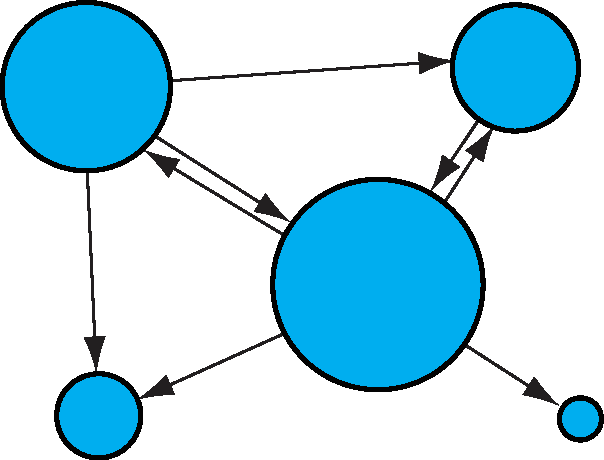
\includegraphics[scale=0.6]{mim/example-migration-lightblue}}
\end{center}
\begin{picture}(0,0)(0,0)
\put(76,50){$M_{14}$}%
\put(75,40){$M_{12}$}%
\put(52,26){$M_{13}$}%
\put(103,20){$M_{15}$}%
\put(89,42){$M_{42}$}%
\put(70,22){$M_{23}$}%
\put(67,32){$M_{21}$}%
\put(102,36){$M_{24}$}%
%
\put(59,45){$\Theta_1$}
\put(89,25){$\Theta_2$}
\put(52,14){$\Theta_3$}
\put(103,48){$\Theta_4$}
\put(115,13){$\Theta_5$}
\end{picture}

\caption{Populations exchanging migrants with rate $m_{j \rightarrow i}$ per generations and with size 
$N_e$. The parameters are scaled by mutation rate $\mu$ which is with sequence data per site per generation. The estimated parameters are therefore: $\Theta_i$ which is $x N^{(i)}_e \mu$ and 
$\M_i$ 
which is $m_i/\mu$, the migration estimate is often also expressed as $xNm$ which is just $\Theta \M$, x is the inheritance parameter and depends on the data, commonly 4 for nuclear data, and 1 for mtDNA data. The example model is not a complete (full) model because some migration routes are not estimated and set to zero.}
\label{FIG1}
\end{figure}



\begin{figure}[tbh]
\begin{center}
\leavevmode
\hbox{%
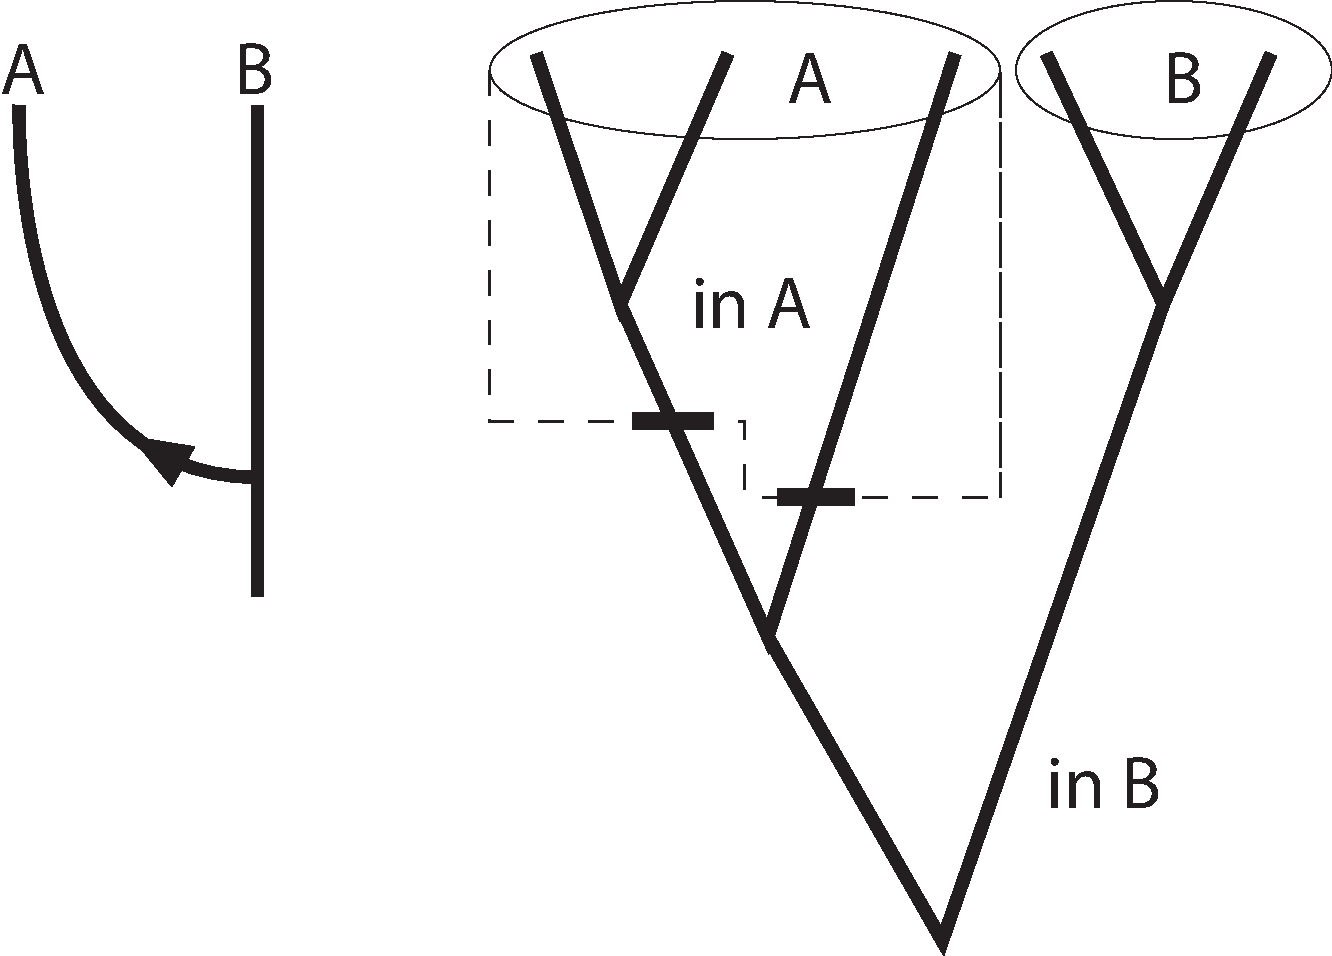
\includegraphics[scale=0.4]{mim/species_manual}}
\end{center}

\caption{Populations splitting, left is the model specification, two populations A and B, A splits off B. Right, detail view for the gene tree. Each individual can split off by itself.}
\label{FIG2}
\end{figure}

\section*{Mutation-scaled population splitting  times $\Delta$ and standard deviations $S_\Delta$}
The population splitting times are model differently to other programs that all use the model of IM \citep{Hey:2010a}.
Our new model was described by \cite{beerli2019b}.  We treat population splitting events as individual events on a lineage. Looking backward in time, a lineage $\ell$  currently in population $\kappa$ is at risk of being  in a different population either by migration with rate $\M$ or into another population by a splitting event. The Splitting event is proposed during the MCMC run using a hazard function of the splitting time distribution, for simplicity we use a truncated Normal distribution with mean $\Delta$ and standard deviation $S_\Delta$. Drawing these splitting events using a hazard function is equivalent to the coalescent or migration event which are also hazard functions. During the MCMC runs many different splitting events will be proposed from the Normal distribution with $\Delta_j$ and $S_{\Delta_j}$ for $j$ population splits. The current version needs guidance which populations are merging (looking backwards in time), for an example see the Bayes Factor section.  In the parmfile and the menu the setting of the splitting parameters is combined with setting the migration model, for an example see definition of the custom migration matrix.  


%\section{Maximum likelihood estimation of migration rates}
%The estimates of the parameters $\P$ are found by maximizing formula (\ref{LIKELIHOOD}.)
%We bias the search path through all trees towards trees with higher likelihoods (Fig. 2)
%and have then to correct for this. The likelihood formula changes to
%\begin{align}
%\frac{L(\P)}{L(\P_0)} &= \frac{1}{m}\sum_i^m\ \frac{ \prob(D\ |\ g_i)\ \prob( g_i\ |\ \P)}
%{\prob(D\ |\ g_i)\ \prob( g_i\ |\ \P_0)}.
%\end{align}
%Such an approach is reasonable because summands with low probabilities
%will contribute very little to the final likelihood. For more information on the base model, you should read \cite{beerli:1999:mle} and \cite{kuhner1995-1421}.
%
%The approximation of the likelihood using a ratio makes it difficult to
%compare different runs of the program. The program reports a likelihood
%that is actually a ratio of likelihoods and since we recalculate the
%parameters for each chain, the values for $\P_0$ are different
%between runs, and therefore it is impossible to compare them. A comparison of the parameters, of course, is still possible.
%An escape of this 
%problem is to run the program using the full model (e.g. $n \times n$ parameters and use the likelihood ratio test for specific scenarios.
%
\section{Bayesian inference}
\migrate estimates the parameters using a Bayesian paradigm (see formula \ref{BAYES}), simulation studies of simple models show that there are few differences with the ML runs, although some combinations of parameters might be be easier to estimate with the Bayesian approach \citep{beerli:2006:CBM}. One of the bigger problems with the Likelihood approach is the effort that has to be made to calculate the confidence intervals of the best estimates, default analyses often led to narrow support intervals thus making researchers overconfident about the explanatory power of their data; the use of the prior distribution seems to make a Bayesian approach less vulnerable to this problem. Bayesian inference is commonly based on Markov chain Monte Carlo (MCMC) because we usually cannot integrate the function of interest analytically or by simple numerical approach. MCMC was described first by \cite{Metropolis:1953:ESC} and refined by \cite{hastings1970-97}. For an introduction see \cite{Hammersley:1964:MCM}or \cite{chib:1995:umh}, 
and see \cite{kuhner1995-1421} for a first application using MCMC in the context of coalescence theory.

\begin{figure}[tbh]
\begin{center}
\leavevmode
\hbox{%

\includegraphics[scale=0.8]{mim/planes_orig}}
\end{center}
\caption{
(A) On an imaginary, infinite likelihood surface  we would need to sample every possible
genealogy and sum all these values which is not possible, but trees with low probability will not contribute much to the final likelihood,  (B) by biasing towards better trees we can sample effectively from those trees with high 
contribution to the final likelihood and can approximate the likelihood (\ref{LIKELIHOOD}).
}
\label{FIG3}
\end{figure}

%In principle, we do not need to integrate at all with MCMC but sample parameter values during the run and build a histogram for the parameters of interest.
Commonly we think of the marginal posterior distribution of each parameter (summing/integrating over all 'nuisance' parameters). We use particular values to drive the MCMC, and in a Bayesian analysis we get them from the Prior distribution, this may help to get good results in situations where the data suggests a very rough landscape of parameter- and tree-space (see Fig. \ref{FIG3} for an example with a smooth surface). \migrate allows using several different prior distributions, some are more appropriate for you data than others. I often suggest to use the uniform prior distribution because it is simple and shows obvious deficiencies in an analysis very quickly, but it also tends to increase the credibility intervals because it supports very large or very small parameter values equally. This may sound as an odd choice because for example we know that the population size of humans never was zero and never was $10^{10}$, so a uniform prior distribution with range 0 to $10^{10}$ does not sound right although such a prior would do fine in an analysis because the data is strong enough to suggest that the posterior probability near a size of zero is close to zero and the probability of a size of $10^{10}$ is also small.
 
%The parameter $r$ is the a uniform random number from (0,1].

\subsection{Prior distributions}
\vskip -0.5cm
\subsubsection{Uniform prior distribution}
The parameters have a uniform distribution between a minimal and a maximal value of the parameters, there is a set of minima and maxima for $\underline{\Theta}$ and $\underline{\M}$.
\migrate calculates the uniform by using
\begin{gather}
\label{UNIPRIOR}
    \prob(\P_i) =  \frac{1}{\P_{max} - \P_{min}} \\
    \intertext{it is implemented using a windowing method with window size $\Delta$, that is preferrably around 1/10 of the whole range.}
    \P_{\mathrm new} =  \P_{\mathrm old} + (2 \Delta r - 1) \begin{cases} \P_{\mathrm new} < \P_{\mathrm min}  &  \P_{\mathrm min} + |\P_{\mathrm min} - \P_{\mathrm new}| \\
     \P_{\mathrm new} > \P_{\mathrm max}  &  \P_{\mathrm max} - |\P_{\mathrm max} - \P_{\mathrm new}| \end{cases}
\end{gather}

\subsubsection{Gamma distribution prior}
The truncated gamma distribution has four parameters $\alpha$, $\beta$, minimum $a$, and maximum $b$. The gamma prior in \migrate is defined through the mean $\mu$, $\alpha$, $a$, and $b$ 
\begin{gather}
\label{GAMMAPRIOR}
% (E^(-(x/\[Beta])) x^(-1 + \[Alpha]) \[Beta]^-\[Alpha])/Gamma[\[Alpha]] mathematica standard Gamma
%
\alpha = \mu / \beta\\
\beta = \text{minimization of the mean of the truncated gamma and the parameter $\mu$}  \\
\prob(\P_i) =  \text{probability of the truncated gamma} 
%    \intertext{it is implemented using a windowing method with window size $\Delta$, that is preferrably around 1/10 of the whole range.}
%    \P_{\mathrm new} =  \P_{\mathrm old} + (2 \Delta r - 1) \begin{cases} \P_{\mathrm new} < \P_{\mathrm min}  &  \P_{\mathrm min} + |\P_{\mathrm min} - \P_{\mathrm new}| \\
%     \P_{\mathrm new} > \P_{\mathrm max}  &  \P_{\mathrm max} - |\P_{\mathrm max} - \P_{\mathrm new}| \end{cases}
\end{gather}



\subsubsection{Exponential prior distribution}
The parameters have a exponential distribution, \migrate calculates three versions\\
\textsl{Simple exponential prior distribution}
\begin{align}
\label{EXPPRIOR}
    \prob(\P_i) &=  \int_0^\infty exp( -P_{i} / P_{\mathrm mean}) / P_{\mathrm mean} d\P_i = exp(- P_{i}/P_{\mathrm mean}) \\
    \P_{\mathrm new} &=  - \P_{\mathrm mean}\ ln(r)
\end{align}
\textsl{Exponential prior distribution with fixed window}
\begin{align}
\label{WEXPPRIOR}
    \prob(\P_i, \P_{\mathrm min}, \P_{\mathrm max}) &=  \frac{\int_{\P_{\mathrm min}}^{\P_{\mathrm max}} exp( -P_{i} / P_{\mathrm mean}) / P_{\mathrm mean} d\P_i}{exp(-P_{\mathrm min}/P_{\mathrm mean}) - exp(-P_{\mathrm max}/P_{\mathrm mean})}\\ 
     &= \frac{exp(-P_{\mathrm min}/P_{\mathrm mean}) - exp(-P_{\mathrm x}/P_{\mathrm mean})}{exp(-P_{\mathrm min}/P_{\mathrm mean}) - exp(-P_{\mathrm max}/P_{\mathrm mean})} \\
    \P_{\mathrm new} &=  - \P_{\mathrm mean}\ ln(\frac{r}{exp(\P_{\mathrm max}/\P_{\mathrm mean})}-\frac{r-1}{exp(\P_{\mathrm min}/\P_{\mathrm mean})}); 
\end{align}
\textsl{Exponential prior distribution with variable window}
\begin{align}
\label{AEXPPRIOR}
    \prob(\P_i | \P'_i,  \P_{\mathrm min}, \P_{\mathrm max}) &=  \frac{2 \int_{\P'_i - \Delta}^{\P'_i + \Delta} exp( -P_{i} / P'_i) / P'_i d\P_i}{exp(1) Csch(\Delta / P'_i)}\\ 
     &= \frac{(exp(\Delta + P_i)/P'_i - exp(1)) Csch(\Delta/\P'_i)}{2 exp(\P_i/\P'_i)} 
     \end{align}
     \begin{align}
    \P_{\mathrm new} &=  \P'_i - \P'_i ln(exp(\Delta/\P'_i) - 2 r Sinh(\Delta / \P'_i))\begin{cases} \P_{\mathrm new} < \P_{\mathrm min}  &  \P_{\mathrm min} + |\P_{\mathrm min} - \P_{\mathrm new}| \\
     \P_{\mathrm new} > \P_{\mathrm max}  &  \P_{\mathrm max} - |\P_{\mathrm max} - \P_{\mathrm new}| \end{cases}
\end{align}

\chapter{Files in \migrate}

\myabstract{\migrate can use many different input methods and output methods, but most of them have a very special purpose, as a minimum you need to supply an input datafile, here called \textsl{infile}.}

%\subsection*{Short description of all files \migrate\ can use or generate}
There are multiple ways to set up things. \migrate\ can use very different ways to manipulate the data and as a result many different files are needed or produced. Minimally, you need the data file, its default name is {\sl infile}, and \migrate\ produces two files that contains results: the \textsl{outfile} (ASCII text file) and a PDF output file that contains the same information (well almost, as you see later). The program produces both formats because for quick checking of results the ASCII file can be opened on the command line or with any text viewer, whereas the PDF file requires a PDF reader, for example for macs Preview.app and for windows NitroPDF; unfortunately modern versions of the standard Adobe Acrobat Reader fail to read the PDF files generated by \migrate correctly -- I will work on porting my PDF writer to a newer system, but this has low priority and will take a while (Older versions of Adobe Reader work fine!) 

\vskip 1cm
\section{Input files}
\begin{center}
\begin{tabular}{l l p{7.0cm} l c}
\hline
Filename & Type & Short description & Necessary?  & Name changeable\\
\hline
infile & Input           & {holds you data} & YES & Yes\\
parmfile  & Input       & {holds options} & - & Yes$^{*}$\\
geofile & Input & {holds a (geographic) distance matrix between the populations} & - & Yes\\
%sumfile    & Input      & {holds the summary statistic of the sampled  genealogies from an earlier run, to rerun some statistics}& - & Yes\\
\hline
datefile & Input & holds the date (default is years) of the sample. When used then you need also to supply a generation time and and a mutation rate per year in the {\tt parmfile} or the Menu. & -$^{**}$ & Yes\\
\hline
%seedfile  & Input       & {holds a random number seed} & - & No\\
%distfile & Input      & {holds a genetic distance matrix} & - & No \\
%catfile   & Input       & {holds categories for mutation rate variation} & - & No\\
%weightfile   & Input     & {holds weights for each site} & - & No\\
\hline
\multicolumn{5}{l}{* Under Unix the parmfile name ca be given as an argument to the program}\\
\multicolumn{5}{l}{** When different sample dates are used then this file is needed}
\end{tabular}
\end{center}
\subsection{Main input files}
\begin{description}
\item{\bf infile} if this file is not present in the current directory 
than the program will ask for a data file, and you can
give the path to it, you need to type the path, which is for Macintosh and Windows users probably rather uncomfortable. In the {\bf menu} or {\bf parmfile} you can specify an other default name for your datafile. 
\item{\bf datefile} When the samples came from different years and you believe that this makes a different specify the date as the time backward from today (for example years before 2007). With this analysis type, you need to specify a mutation rate in the same units as the dates of the samples.
%\item{\bf sumfile} The sumfile allows the reuse of a previous maximum likelihood run (see more under sumfile in the output file section), the data type menu needs to be set to "Genealogy".
\item{\bf bayesallfile} The  \texttt{bayesallfile}  or  \texttt{bayesallfile.gz} allows to reuse a previous Bayesian inference run, the parmfile needs to have the option \\
\texttt{recover=YES}\\
This option cannot be created with the menu.
All the other options in the parmfile should be the same as when the \texttt{bayesallfile} was created.
\end{description}
\subsection{Optional input files}
\begin{description}
\item{\bf parmfile} can hold specific menu options, this file and the possible options for the menu are explained in detail in section {\bf menu and parmfile}.
%\item{\bf seedfile} holds a random number seed, this is just present for compatibility with PHYLIP, the random number seed can be set in various
%ways either in the menu or in the parmfile. [this random number seed option should not be used]
\item{\bf geofile} holds the geographic or arbitrary distances between the populations. When this is used then the migration rates are not only scaled by the mutation rate but also by this distance. This allows to detect environmental barriers when we assume that the genetic potential to migrate is the same in all populations; without a barrier the rates should be all the same per distance unit. The format is like a distance file in the PHYLIP package \citep{Felsenstein}, but you can use the {\tt \#} as a commentary character.\\
\begin{small}
\begin{verbatim}
# Example geofile for 3 populations, 
# the order of the population must be the same as in the data file
# 
  3
Tallahasse0.0 10.0 150.0
St.Marks  10.0 0.0 160.0
Pensacola 150.0 160.0 0.0
\end{verbatim}
\end{small}
The example scales the mutation-scaled migration rates by the 'geographic' distance. If the migration rate is linear with the inverse of the distance then the migration rates between all locations will be the same, here we scale the migration rate per distance unit, therefore if we have a range of 0 to 160 miles, the rates are are scaled per mile. As a result migration rates will be all relatively high because a mile is usually not a large distance for vagile species. 
%\item{\bf distfile} holds distances between all individuals (need to be in the same order as the data file). The distance file has the same format as the PHYLIP distance file format. Use this only if you suspect that \migrate\ does not recover from its own UPGMA start tree. [This option should probably not be used for data analysis.]

%\item{\bf catfile} hold the categories. For each locus you must give
%the number of categories, and the value of each category and then a string of
%category assignments for each site. You can use the {\tt \#} as a commentary character.\\
%\begin{small}
%\begin{verbatim}
%# Example catfile for two loci with 40 and 30 bp each
%#
%2 1 10  1111111111111111111122222222222222222222
%3 1 3 9 111111111122223333333333222222
%\end{verbatim}
%\end{small}
%\item{\bf weightfile}, for each site and locus you need to give a weight, acceptable weights are
%integers from 0 - 9 and letters A-Z, A is the weight 10, B 11 and so on, in total
%there are 35 possible different weights possible. { You need  a weight string for
%each locus}. [if you use this option please let me know]\\
%\begin{small}
%\begin{verbatim}
%# Example weightfile for two loci with 40 and 30 bp each
%# 
%1101101101101101101101101101101101101101
%33F33F22F22F22F22F22FHHHHHHHHH
%\end{verbatim}
%\end{small}
%\end{description}
\newpage
\section{Output files}
\begin{center}
\begin{tabular}{l p{8.0cm} l c}
\hline
Filename & Short description & Name changeable\\
\hline
parmfile     & {holds options, menu can rewrite this file}  & see menu\\
outfile           & {will be created and replace any file with the same name in the same directory}  & Yes\\
outfile.pdf          & contains the same output as outfile and histograms, you need a PDF viewer to read this file  & Yes\\
bayesfile & contains the histogram data of a Bayesian run (the outfile.pdf used these to generate the posterior distributions. & Yes\\
bayesallfile & contains the raw data of a Bayesian run, can be run through TRACER when only a single replicate and a single locus is used. & Yes\\
mighistfile &  contain the distribution of migration events over time. & Yes\\
skylinefile &  contains the distribution of the parameter values over time as calculated by using the expected parameter values for a short time intervals. & Yes\\
treefile         & {holds genealogies, this file will be created and will replace any file with the same name in the same directory} & No\\
%mathfile        & {holds plot coordinates for the use in a mathematica notebook, this file will be created and will replace any file with the same name in the same directory} & Yes\\
%sumfile         & {holds the summary statistic of the sampled  genealogies for further analysis, this file will be created and will replace any file with the same name in the same directory} & Yes\\
logfile  &  {logs the progress information that is displayed onto the screen into a file} & Yes\\
\hline
\end{tabular}
\end{center}
\subsection{Main output files}
Some conbination of the output files are not possible, for example a standard Bayesian run will not fill values into the treefile, etc.
\begin{description}
\item{\bf outfile} and {\bf outfile.pdf}  Somewhere you want to read the results, that is it! The name \textbf{outfile} is the default, but can be changed either in the menu or the parmfile. The PDF file contains graphical representation of some of the table and values. Currently, most of the output is represented in the PDF file, when you used the Bayesian inference setting, with Maximum likelihood there are still some options that are not supported in the PDF file (I still lack a programmer to do all this).
\end{description}
\begin{description}
\item{\bf treefile} holds all, only those of the last chain, or 
the best tree(s). The likelihood of each tree is given ($\prob(\mathcal D\ |\ \G)$) in a comment. The programs writes trees with migrations using the Newick format with extensions from the Nexus format. Such trees containing migration events can be printed using the program \texttt{Eventtree} (or short \texttt{ET}) (distributed from http://popgen.scs.fsu.edu/et).
Writing trees to a treefile adds
some burden to the program, it will run slower, especially with the option BEST. Parallel runs increase the communication with the master node and therefore may slow down your run. 

%\item{\bf mathfile [ML only]} holds the raw likelihood surface data, if this was requested in the options. The name mathfile is the default, but can be changed in the menu or parmfile (see appendix). This option seems to produce crashes on some parallel runs. Do not use it on Bayesian inference runs either because the data for the mathfile does not get filled in, this may appear at one time because the plot function that fills in the mathfile could in principle show posterior distributions of all immigrations and all ``emigrations" (this means only the emigrants that successfully arrive at the other populations in the study).
%
%\item{\bf sumfile [ML only]} holds the summaries of all genealogies, if this was requested in the parmfile or menu. The name \textbf{sumfile} is the default. This option allows you to reanalyze a previous run for likelihood ratio test or profile likelihoods.

\item{\bf bayesfile} holds the posterior histogram data show in the PDF files. You can use other program packages like the matplotlib package in python (http://www.python.org), GNUPLOT (http://www.gnuplot.org), or the GMT package (http:www.soest.hawaii.org/gmt2) to recreate the histograms.
\item{\bf bayesallfile} holds the raw posterior values for all parameters. This option reduces the memory footprint by writing all intermediate results to disk and then rereads them for summarizing and printing the final results. This file can be also used to independently test whether \migrate converged or not using the program \tracer \citep{Rambaut:2007,Drummond:2007}, \migrate uses a simple 1-step Effective sample size (ESS) calculator that may not always be very accurate, although comparison showed that seeing high autocorrelation in \migrate means to see high autocorrelation (small ESS) in \tracer.

\item{\bf mighistfile} holds the histogram over time of the frequency of migration and coalescence events, with simulated data these plots show typically an exponential decay. When there were changes of parameters over time then the data will enforce different patterns, that can be used to discuss the results.

\item{\bf skylinefile} holds the averages of the expected parameter values at specific times. These plots are similar to the skyline plot reported in \beast \citep{Drummond:2005:BCI}, although their derivation is an extension of the original skyline plots of \citep{strimmer:2001:EDH}. \migrate reports changes of population sizes and migration rates over time and summarizes over multiple loci. 
\end{description}

% !TEX root = migratedoc.tex
\chapter{Data models}

\myabstract{A short overview of the different datatypes and how multiple loci are summarized.}

\migrate\ allows for several different input data types, such as electrophoretic marker data, microsatellite data, sequence data as stretches of contiguous sites and as single nucleotide polymorphisms.
 
\section{Infinite allele model}
This assumes 
that every 
mutation will 
result in a new 
allele, there is no back mutation (Fig. \ref{EPFIG}). This model is used in all current implementations of electrophoretic data analyses packages (Biosys-1, GDA among others)
and perhaps is appropriate for this kind of data. \migrate is calculating the parameters for 
each locus independently and summarizes at the end taking the likelihood surfaces or Posterior distributions of each locus into account.
\begin{figure}[thb]
\begin{center}
\makebox[1in]{

\includegraphics[scale=0.6]{mim/ep_graph}}
\end{center}
\caption{Left: Mobility of electrophoretic marker in an electric field. the alleles a,b,c,.. describe a possible sequence of mutation, their mobility is not correlated with the mutational history. Right: The probability that a given allele is not mutating during some time, 
this is a simple exponential relationship.}
\label{EPFIG}
\end{figure}
%\afterpage{\clearpage}
\newpage
\section{Microsatellite model}
\subsection{Ladder model}
The ladder model was invented by cite{ohta:1973:amm} and \cite{kimura:1978:ste} for electrophoretic markers, but was  not as good as expected in describing real electrophoretic alleles. For microsatellites this model seems
much more appropriate cite[e.g. ][]{valdes:1993:afm}, but see \cite{rienzo:1994:mps}, here obviously change happens mostly by slippage of the two DNA strands
creating with higher probability a new allele which is only 1 step apart from the old than one
which 2 steps apart (Fig. \ref{MSATFIG}). 
\begin{figure}[thb]
\begin{center}
\makebox[1in]{

\includegraphics[scale=0.6]{mim/msat_graph}}
\end{center}
\caption{Left: Number of repeat changes of a microsatellite marker. The probability to have a slippage of only one repeat is higher than the slippage of more than one repeat, in a given time, here time=0.1. Right: The probability that a change of 0,1,2,.. steps is occurring during some time.}
\label{MSATFIG}
\end{figure}
%\afterpage{\clearpage}

\subsection{Brownian motion approximation to the ladder model}
This replaces the discrete stepwise mutation model with a continuous Brownian motion model
The results are very similar to the exact stepwise mutation model, but the parameter
estimation is several times faster. This is a crude approximation that has some difficulties when the dataset is not very variable because it uses a cutoff for the the probability that there is no change between two points on a branch, during a time of x  the Brownian motion approximation replaces discrete jumps between repeats with a continuous approximation.
\begin{figure}[thb]
\begin{center}
\makebox[1in]{
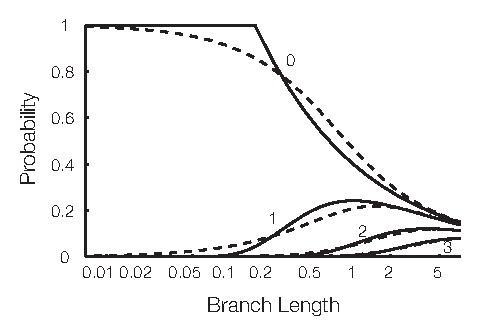
\includegraphics[height=2in]{mim/brownian-stepwise}}
\end{center}
\caption{Comparison of stepwise mutation model with Brownian motion approximation (dashed lines).  The numbers 0, 1, 2, 3, 4 are the number of steps. The Brownian motion approximation for no change is truncated at 1. With steps of more than 4 there is no differences between the stepwise model and the approximation. X-Axis is in log$_10$}
\label{BROWNFIG}
\end{figure}

 
\section{DNA/RNA model}
\subsection{Sequence model}
Migrate implements the sequence model of Felsenstein (1984)  available in {\texttt{dnaml}} (PHYLIP 4.0, Felsenstein 1997)(Fig. \ref{SEQFIG}). The transition probabilities were published by Kishino and Hasegawa (1989).  {\migrate} does not allow for recombination within a locus and therefore may over-estimate variability because of recombination, but this bias is not explored well, if in doubt I suggest to try to run \migrate, simulated high recombination rate data leads to difficulties with convergence. Applications of recombination tests beforehand may work well, but most of these recombination recognition program use the 4-gamete test that is based on the infinite sites model and therefore will overestimate the importance of recombination.\\
Like {\texttt{dnaml}}, {\migrate} also allows for different evolutionary rates, mutation categories and autocorrelation, although
any use of these additional features can slow done to program to a crawl, but this may change
in the future as computers double their speed roughly every 2 years.
\begin{figure}[b]
\begin{center}
\makebox[1in]{

\includegraphics[scale=0.7]{mim/seq_graph}}
\end{center}
\caption{Left: Sequence mutation model. 
Transitions are are shown in black lines, transversion are 
shown with dotted lines.
Right: The probability that a transition or transversion is occurring during some time.
The shown graph uses equal base frequencies, but the used model does not need this restriction.}
\label{SEQFIG}
\end{figure}
%\afterpage{\clearpage}
\subsection{Single nucleotide polymorphism data (SNP)}
We use a rather restrictive ascertainment 
models for SNPs \cite{kuhner:2000:usn}. A better approach than using SNPs is the use of short reads which may or many not contain SNPs. I find that SNPs are an inferior datatype because commonly researchers are adding criteria such as a minor SNP allele must occur at a frequency higher than $x$, and singletons are excluded etc. 
%Currently there are two versions implemented. 
%If you want to use the SNP options, please contact me before
%you run large scale analyses. 
\begin{enumerate}
\item We have
found ALL variable sites and use them even if there are only a few
members of another alleles present. In principal it is as you would
sequence a stretch of DNA and then remove the invariant sites.
Each stretch is treated as completely linked. You can combine many of 
such ``loci'' to improve your estimates.
%\item SNP were developed from a panel population of which we know the
%number of individuals, and that the markers developed were variable, but
%we do not know the actual nucleotides for the individuals [Not fully tested].
\end{enumerate}
This is certainly not how people develop SNPs, but currently the closest
we can come up with.
The SNP coding is otherwise exactly the same as the coding for DNA data.
\par
%If you want to assume that each SNP is unlinked then you need to 
%code each SNP like a sequence data locus with one nucleotide
%(see the examples for sequences),
%I have run successfully 50 SNP loci on a laptop using 40 MB of RAM.
%But there may be better ways to run loci consisting of only one site.

\section{Combining multiple loci}
\migrate calculates all loci estimates independently, the multi-locus estimate is not a simple average over all loci, but takes into account the likelihood or posterior distribution for each parameter at each locus. Loci with flat likelihood curves or flat posteriors will not contribute as much as those with strongly peaked distributions. \migrate offers different treatment in the mutation menu of the parameter menu for the mutation rate among loci:
\begin{center}
\begin{minipage}[c]{12cm}
\begin{verbatim}
Mutation rate among loci
(C)onstant    All loci have the same mutation rate [default]
(E)stimate    Mutation rate 
(V)arying     Mutation rates are different among loci [user input]
(R)elative    Mutation rates estimated from data
\end{verbatim}
\end{minipage}
\end{center}
The {\textbf{Constant}} assumption forces each locus to have the same identical mutation rate. Try this first, because it is the least complicated and most often gives fine results. The {\textbf{Estimate}} is the most difficult and needs dated samples, without sample dates do not use this option.
%one and may often fail, because your data does not contain many loci, or the run has some some loci that did not converge well. With Maximum likelihood this option tries to fit a gamma distribution with a parameter alpha assuming that there is a mean mutation rate for all loci with a rate modifier with shape parameter $\alpha>0$ and $\beta = 1.0$. This results in allowing for variation among loci due to mutation. This often is very difficult to run to convergence. Bayesian inference tries to estimate the rate modifier for each locus, but this seems to work only when information about the dates of the samples is present, and even then it may fail [this needs more work]. 
The last two options, {\textbf{Varying and Relative}}, are probably the best ones to try if you really need variable mutation rates. When you know the relative differences of mutation rates in your data, you can specify them. Alternatively, let \migrate estimate the relative mutation rate using your data. For sequences \migrate calculates a simple Watterson's effective population size estimate over all samples and for each locus and then uses that to calculate a relative mutation rate. With microsatellites and allozyme data \migrate counts the number of alleles and uses those as a measure of relative mutation rates. The mean of these rates is 1.0.
\newpage

\def\startformatted{%
\begin{flushleft}
\begin{small}
\begin{tt}}

\def\endformatted{%
\end{tt}
\end{small}
\end{flushleft}
}%

\chapter{Data file specification}
\unitlength=1mm
\begin{picture}(0,0)(0,0)
\put(110,-12){
\includegraphics[width=6cm]{mim/read}}
\end{picture}

\myabstract{In detail specification of the data format, without reading and using this information your analysis will most likely faulty.} 

The data needs to be in  a certain form; for us, the following formats were most convenient, but you need to edit your data into this form.
There are some programs that can write \migrate files, for example the  program \textsc{MSAanalyzer} \citep{dieringer:2003} that can generate \migrate datafiles from excel spread sheets for microsatellite data. The following formats are discussed in detail:
\begin{itemize}
  \item DNA or RNA sequence data (single locus and multilocus)
  \item Single nucleotide polymorphism data (two formats)
  \item Microsatellite marker data (\migrate uses {\bf REPEATNUMBERS by DEFAULT!!!!!!!})
  \item Allozyme data (or other infinite allele mutation model marker)
\end{itemize}
\vskip 1cm
\section*{General data format}
Syntax: a token is either a word, a collection of words, or a character or a number:
\begin{description}
\item{$<token>$} the token between the the ``angle-brackets" is obligatory
\item{$\left[token\right]$} in square brackets are optional.
\item{$\left\{token\right\}$} are obligatory for some 
\item{$<token1 | token2>$} choose one of the token kind of data.
If this is too abstract, look at the examples further down.
\end{description}
A range of numbers in a ``word" token as in $<${\tt individual1 10-10}$>$
means that this token needs to be 10 characters long. The characters for
any word token can normally include special characters, punctuation, and spaces, the token for the individual name ``{\tt Ind1  02 @}" is legal. An explanation of the individual parts follows at the end of this section.
The most common data file for allozyme data or microsatellite data
would look like this (examples follow):
\smallskip
\begin{small}
\begin{tt}
\begin{verbatim}
<Number of populations> <number of loci> {delimiter between alleles} [project title 0-79]
{#@M <msat1-repeatlength> <msat2-repeatlength> .....}
<Number of individuals> <title for population 0-79>
<Individual 1 10-10> <data>
<Individual 2 10-10> <data>
....
<Number of individuals> <title for population 0-79>
<Individual 1 10-10> <data>
<Individual2 10-10> <data>
....
\end{verbatim}
\end{tt}
\end{small}
The delimiter is needed for microsatellite data and the project title is optional.  The line starting with {\tt \#@M}  is not necessary when the data consists of allozyme data or microsat repeat numbers. The line allows to automatically calculate the number of repeats from the fragment length.   The {\tt data}
will be described in the following sections. \textbf{The population name must start with a alphabetical character (not a number). The individual name has to be  10 characters by default} (same as in PHYLIP), but can be changed to another constant in the parmfile, even to a length of 0.
[This is one of the most common errors, make sure that your individual names are 10 characters, it does not matter whether they are all alphanumeric, spaces are fine]
\par
For sequences or SNPs, the syntax is slightly different, the following case 
is for non-interleaved sequence data.
 \begin{small}
\begin{tt}
\begin{verbatim}
<Number of populations> <number of loci> [project title 0-79]
<number of sites for locus1> <number of sites for locus 2> ...
<Number of individuals locus1> <#ind locus 2> ... <#ind loc n> <title for population 0-79>
<Individual 1 10-10> <data locus 1>
<Individual 2 10-10> <data locus 1>
....
<Individual 1 10-10> <data locus 2>
<Individual 2 10-10> <data locus 2>
....
<Number of individuals>  <#ind locus 2> ... <#ind loc n>  <title for population 0-79>
<Individual 1 10-10> <data locus 1>
<Individual 2 10-10> <data locus 1>
....
<Individual 1 10-10> <data locus 2>
<Individual 2 10-10> <data locus 2>
....
\end{verbatim}
\end{tt}
\end{small}
%Earlier versions of MIGRATE (before 1.5.2) would not allow to have different numbers of individuals for different loci and its syntax was:
%\begin{verbatim}
%<Number of individuals> <title for population 0-79>
%\end{verbatim}
For each locus one can give different number of individuals, if there is only one number then the program assumes that all loci have the same number of individuals. If there a fewer numbers than loci
the last number will substitute for the number of individuals at the other loci. It is important that the population name does not start with a number!
\smallskip
\migrate version older than 4.0 supported interleaved sequence formats, Ivstopped supporting this and have therefore removed its description, reformat your data to a non-interleaved format before you translate it into the \migrate format. I typically use \textsc{Paup*} \cite{swofford2003} to export a non-interleaved \phylip formatted datafile and use that to change into the \migrate format.
%Interleaved sequence data [IMPORTANT, do no add blank lines into the infile, \migrate\ will choke on those, although they will run in other programs]:
%\smallskip
%\begin{small}
%\begin{tt}
%\begin{verbatim}
%<Number of populations> <number of loci> [project title 0-79]
%<number of sites for locus1> <number of sites for locus 2> ...
%<Number of individuals locus 1>  <#ind locus 2> ... <#ind loc n> <title for population 0-79>
%<Individual 1 10-10> <data locus 1 part 1>
%<Individual 2 10-10> <data locus 1 part 1>
%....
%<data ind1 locus 1 part 2>
%<data ind2 locus 1 part 2>
%....
%<Individual 1 10-10> <data locus 2>
%<Individual 2 10-10> <data locus 2>
%....
%<data ind1 locus 2 part 2>
%<data ind2 locus 2 part 2>
%....
%etc.
%\end{verbatim}
%\end{tt}
%\end{small}
\vskip 0.5cm
A data type called \textbf{HapMap} is available for SNP data that allows less cumbersome input of SNP data than old versions of \migrate, but see current imput format.
You still can use a single site as a locus (SNP), but with many loci this will be difficult to manage. The HapMap data type uses this format:
 \begin{small}
\begin{tt}
\begin{verbatim}
<Number of populations> <number of loci> [project title 0-79]
<Any Number> <title for population 0-79>
<Position on chromosome locus1> <TAB><allele><TAB><number><TAB><allele><TAB><number><TAB><total>
<Position on chromosome locus2> <TAB><allele><TAB><number><TAB><allele><TAB><number><TAB><total>
....
<Any Number>  <title for population 0-79>
<Position on chromosome locus1> <TAB><allele><TAB><number><TAB><allele><TAB><number><TAB><total>
<Position on chromosome locus2> <TAB><allele><TAB><number><TAB><allele><TAB><number><TAB><total>
....
\end{verbatim}
\end{tt}
\end{small}
The current format assumes that each SNP is biallelic. $<$allele$>$ contain the nucleotide and the $<$number$>$ contains the number of individuals with that specific allele, the total number is the sum of both,
and is currently not necessary, but I may use this later to accommodate slight extension of this format, currently the total number is read from the program but not further used. This format will extend to more useful analyses that take into account the position on the chromosome, but this is currently not used.
\subsubsection{Summary of the individual tokens}
\begin{entry}{5cm}
\item[\token{Number of populations}] Number of populations. Range: $1, 2, 3, \dots, n$ where $n$ is a smallish number, remember that the default \migrate run estimates $n^2$ parameters.
\item[\token{Number of Loci}] Number of unlinked loci. Range: $1, 2, 3, \dots, \ell$ where $\ell$ can be a large number.
\item[\token{Delimiter}] can be any character that does not occur in some other function in the data set, examples: @ , . /
\item[\token{Number of individuals}] Number of individuals within one population.  Range: $1, 2, 3, \dots, m$. For exploring \migrate I suggest to use around 10 to 20 individuals, much less (for example 1 or 2) or more (for example 1000) will make the analysis more difficult and need more experience and patience. 
\item[\token{Title for population}] Title for the population, the first letter must \textbf{not be a Number}!
\item[\token{Individual}]  Remember that the default for individual names needs 10 characters. Ideally, each individual name is unique and the first letter of the individuals name represents a code for the populations, for example $0,1,2,..$  
\item[\token{Data}] See examples for the different data types.
\item[\token{Number of sites}] Number of linked sites.  Range: $1, 2, 3, \dots, S$ 
\item[\token{Position on Chromosome}] Location on genome measured in sites [not functional yet]
\item[\token{Allele}] For SNP data this is one of the nucleotides: A, C, G, T.
\item[\token{Number}] For SNP data this is the number of $<$Allel$>$ at that specific site in the sample. 
\item[\token{Total}] For SNP data this is the total number of  samples at the specific site. 
\end{entry}

\subsection{Examples of the different data types}
The examples in this section look like real data, but they are only
for the demonstration of the syntax, if you try run this ``data''
it will deliver often very strange values, I have added a ``usable'' test set
of simulated data in the examples directory, see the file examples/README 
for more information.
\subsubsection{Allozyme data (infinite allele model)}
\begin{picture}(0,0)(0,0)
\put(175,-30){\rotatebox{90}{\Large ALLOZYME}}
\end{picture}\hskip -0.5mm
The data is given in genotypes, any printable character with ASCII
code bigger than 33 ('!') and smaller than 128 can be used. '?' is reserved for missing data. You can use multi-character coding when you use a delimiter (see the
examples for microsatellites).
If there is enough interest I can work on a input using
gene frequencies, although I prefer to work on more interesting things than adjusting input files.
\smallerskip
Most simple example with a single locus, 2 population and 5 total individuals. 
\begin{flushleft}
\begin{small}
\begin{tt}
\begin{verbatim}
 2 1 Migration rates between two Turkish frog populations
3 Akcapinar (between Marmaris and Adana)
PB1058    ab 
PB1059    ab 
PB1060    b? 
2 Ezine (between Selcuk and Dardanelles)
PB16843   ab 
PB16844   bb 
\end{verbatim}
\end{tt}
\end{small}
\end{flushleft}
\smallerskip
Example with 2 populations and 11 loci and with  3 and 2 individuals per population,
respectively (this data set is only an example of syntax, analyzing this
dataset would not make much sense).
\begin{flushleft}
\begin{small}
\begin{tt}
\begin{verbatim}
 2 11 Migration rates between two Turkish frog populations
3 Akcapinar (between Marmaris and Adana)
PB1058    ee bb ab bb bb aa aa bb ?? cc aa 
PB1059    ee bb ab bb bb aa aa bb bb cc aa 
PB1060    ee bb b? bb ab aa aa bb bb cc aa 
2 Ezine (between Selcuk and Dardanelles)
PB16843   ee bb ab bb aa aa aa cc bb cc aa 
PB16844   ee bb bb bb ab aa aa cc bb cc aa 
\end{verbatim}
\end{tt}
\end{small}
\end{flushleft}
\smallerskip
Same example, but with a different syntax that allows multicharacter allele names (see last locus!). The delimiter is specified as the third parameter in the first line, the delimiter cannot be a standard alphabet character. 
\begin{flushleft}
\begin{small}
\begin{tt}
\begin{verbatim}
 2 11 / Migration rates between two Turkish frog populations
3 Akcapinar (between Marmaris and Adana)
PB1058    e/e b/b a/b b/b b/b a/a a/a b/b ?/? c/c Rs/Rf 
PB1059    e/e b/b a/b b/b b/b a/a a/a b/b b/b c/c Rs/Rs 
PB1060    e/e b/b b/? b/b a/b a/a a/a b/b b/b c/c Rs/Rs 
2 Ezine (between Selcuk and Dardanelles)
PB16843   e/e b/b a/b b/b a/a a/a a/a c/c b/b c/c Rf/Rf
PB16844   e/e b/b b/b b/b a/b a/a a/a c/c b/b c/c Rf/Rs 
\end{verbatim}
\end{tt}
\end{small}
\end{flushleft}

\subsection{Microsatellite data}
\begin{picture}(0,0)(0,0)
\put(175,-50){\rotatebox{90}{\Large MICROSATELLITE}}
\end{picture}\hskip -0.5mm
{\bf DEFAULT INPUT SYNTAX}\\
The third argument on the first line has to be a delimiter character, for example a {\bf ``."}.
The data is given in genotypes. Each individual has two alleles.
Alleles are coded as \textbf{REPEAT NUMBERS}, so for example your 
sequence 
\begin{verbatim}
Flanking    msat    Flanking
region              region 
--------============-------
ACCTATAGCACACACACACAAATGCGA      6 CA repeats
ACCTATAGCACACACACA--AATGCGA      5 CA repeats
\end{verbatim}
contains a microsatellite with 6 repeats. And if with a homozygote individual
it needs to be coded as 6.6 or 06.06, where the ``,'' is the delimiter. 
 '?' is reserved for missing data.
\smallerskip
Example:
\begin{flushleft}
\begin{small}
\begin{tt}
\begin{verbatim}
 2 3 . Rana lessonae: Seeruecken versus Tal
2   Riedtli near Guendelhart-Hoerhausen
0         6.5 37.31 18.18
0         6.6 37.33 18.16
2  Tal near Steckborn
1         4.5 35.? 18.18 
1         4.4 35.31 20.18 
\end{verbatim}
\end{tt}
\end{small}
\end{flushleft}

{\bf FRAGMENT LENGTH INPUT SYNTAX}\\
{\bf Earlier version of }
The third argument on the first line has to be a delimiter character, for example a {\bf ``."}.
The data is given in fragmentlength. Each individual has two alleles.
Alleles are coded as \textbf{FRAGMENTLENGTH}, so for example your 
sequence 
\begin{verbatim}
Flanking    msat    Flanking
region              region 
--------============-------
ACCTATAGCACACACACACAAATGCGA      27 sites total length
ACCTATAGCACACACACA--AATGCGA      25 sites total length
\end{verbatim}
contains a microsatellite with 6 repeats, but you only have measures of the total length, here for the first allele there are 27 sites and the second allele there are 25 sites. This format needs an additional line to tell \migrate that we use fragment length and that \migrate needs to do the translation to repeat numbers, inspect closely the line that starts with \#@M in the example below. The \#@M tells the program that here comes a definition of the 
microsatellite repeats, and the numbers force \migrate to assume that the loci are dinucleotide repeats (2) , ot trinuleotide with 3 or tetranulceotides with 4 nucleotides per repeat, and so forth. 

And if with a homozygote individual
it needs to be coded as 25.25 or 025.025, where the ``.'' is the delimiter. A heterozygote would read 25.27, for example.
 '?' is reserved for missing data.
\smallerskip
Example:
\begin{flushleft}
\begin{small}
\begin{tt}
\begin{verbatim}
  2 3 . Rana lessonae: Seeruecken versus Tal
#@M 2 2 2
2   Riedtli near Guendelhart-Hoerhausen
0         25.27 137.131 218.218
0         27.27  218.216
2  Tal near Steckborn
1         23.25 135.? 218.218 
1         23.23 135.131 220.218 
\end{verbatim}
\end{tt}
\end{small}
\end{flushleft}
\subsection{Sequence data}
The sequence data format has received a face-lift: two new formats are now allowed (1) the old format described below and (2) the new format that is more appropriate for genomic type data.

After  the individual name 
follows  the  base  sequence  of  that species, each character being one of the 
letters A, B, C, D, G, H, K, M, N, O, R, S, T, U, V, W, X, Y, ?, or - .  Blanks will be ignored, and so 
will  numerical  digits.   This  allows GENEBANK and EMBL sequence entries to be 
read with minimum editing.      These characters can be  either  upper  or  lower  case.   The  algorithms 
convert  all  input  characters  to upper case. 
The characters constitute the IUPAC (IUB) nucleic acid code  plus  some  slight 
extensions (Table \ref{iupac}).  They enable input of nucleic acid sequences taking full account of 
any ambiguities in the sequence.   
\begin{table}[hpbt]
\caption{IUPAC (IUB) convention for naming nucleotide sites and ambiguous sites} \label{iupac}                                            
\begin{center}
\begin{tabular}{lll c lll}        
\hline                                                                
Symbol & Meaning  & && Symbol & Meaning\\
\hline            \\                                                   
A & Adenine      & && B & not A & (C or G or T)  \\                                                   
G & Guanine      & &&D & not C & (A or G or T)\\                                             
C & Cytosine      &&& H & not G & (A or C or T) \\                                           
T & Thymine       &&& V & not T & (A or C or G)\\                                             
U & Uracil        &&&X,N,? & unknown & (A or C or G or T)\\                                          
Y & pYrimidine & (C or T)  &&O & deletion              \\                                      
R & puRine & (A or G)   &&- & deletion   \\                                 
W & "Weak" & (A or T)      \\                                 
S & "Strong" & (C or G)    \\                                  
K & "Keto" & (T or G)      \\                              
M & "aMino" & (C or A)     \\                                
\end{tabular}
\end{center}
\end{table}

Most simple example with 1 population and a DNA-locus with 50 basepairs.
\begin{flushleft}
\begin{small}
\begin{tt}
\begin{verbatim}
   1 1 Make believe data set using simulated data (1 locus)
50 
3  Tallahassee 
Peter     ACACCCAACACGGCCCGCGGACAGGGGCTCGAGGGATCACTGACTGGCAC
Donald    ACACAAAACACGGCCCGCGGACAGGGGCTCGAGGGGTCACTGAGTGGCAC
Christian ATACCCAGCACGGCCGGCGGACAGGGGCTCGAGGGAGCACTGAGTGGAAC
\end{verbatim}
\end{tt}
\end{small}
\end{flushleft}
\begin{flushleft}
\begin{small}
\begin{tt}
\begin{verbatim}
   1 1 Make believe data set using simulated data (1 locus) OLDFORMAT
50 
3  Tallahassee 
Peter     ACACCCAACACGGCCCGCGGACAGGGGCTCGAGGGATCACTGACTGGCAC
Donald    ACACAAAACACGGCCCGCGGACAGGGGCTCGAGGGGTCACTGAGTGGCAC
Christian ATACCCAGCACGGCCGGCGGACAGGGGCTCGAGGGAGCACTGAGTGGAAC
\end{verbatim}
\end{tt}
\end{small}
\end{flushleft}
The new format looks very similar in its simplest version
\begin{flushleft}
\begin{small}
\begin{tt}
\begin{verbatim}
   1 1 Make believe data set using simulated data (1 locus) NEWFORMAT
(s50) 
3  Tallahassee 
Peter     ACACCCAACACGGCCCGCGGACAGGGGCTCGAGGGATCACTGACTGGCAC
Donald    ACACAAAACACGGCCCGCGGACAGGGGCTCGAGGGGTCACTGAGTGGCAC
Christian ATACCCAGCACGGCCGGCGGACAGGGGCTCGAGGGAGCACTGAGTGGAAC
\end{verbatim}
\end{tt}
\end{small}
\end{flushleft}

\smallerskip
Same example, but now with 2 population and a single DNA-locus with 50 basepairs.
\begin{flushleft}
\begin{small}
\begin{tt}
\begin{verbatim}
   2 1 Make believe data set using simulated data (1 locus) OLDFORMAT
50 
3  Tallahassee 
Peter     ACACCCAACACGGCCCGCGGACAGGGGCTCGAGGGATCACTGACTGGCAC
Donald    ACACAAAACACGGCCCGCGGACAGGGGCTCGAGGGGTCACTGAGTGGCAC
Christian ATACCCAGCACGGCCGGCGGACAGGGGCTCGAGGGAGCACTGAGTGGAAC
3  St. Marks 
Lucrezia  ACACCCAACACGGCCCGCGGACAGGGGCTCGAGGGATCACTGACTGGCAC
Isabel    ACACAAAACACGGCCCGCGGACAGGGGCTCGAGGGGTCACTGAGTGGCAC
Yasmine   ATACCCAGCACGGCCGGCGGACAGGGGCTCGAGGGAGCACTGAGTGGAAC
\end{verbatim}
\end{tt}
\end{small}
\end{flushleft}
In the new format this still looks very similar to the old format except for the line that contains the number of sites,
the simple number of sites is replaced by the data type 's' and the parenthesis specifies that the locus is unlinked


More complicated example with 2 population AND with {\bf 2 loci}, the sequences are NOT interleaved, I drop the interleaved from because I find it error-prone cumbersome to change and unnecessary.
\begin{flushleft}
\begin{small}
\begin{tt}
\begin{verbatim}
   2 2 Make believe data set using simulated data (2 loci) OLDFORMAT
50 46 
3 3   pop1 
eis       ACACCCAACACGGCCCGCGGACAGGGGCTCGAGGGATCACTGACTGGCAC
zwo       ACACAAAACACGGCCCGCGGACAGGGGCTCGAGGGGTCACTGAGTGGCAC
drue      ATACCCAGCACGGCCGGCGGACAGGGGCTCGAGGGAGCACTGAGTGGAAC
eis       ACGCGGCGCGCGAACGAAGACCAAATCTTCTTGATCCCCAAGTGTC
zwo       ACGCGGCGCGAGAACGAAGACCAAATCTTCTTGATCCCCAAGTGTC
drue      ACGCGGCGCGAGAACGAAGACCAAATCTTCTTGATCCCCAAGTGTC
2    pop2
vier      CAGCGCGCGTATCGCCCCATGTGGTTCGGCCAAAGAATGGTAGAGCGGAG
fuef      CAGCGCGAGTCTCGCCCCATGGGGTTAGGCCAAATAATGTTAGAGCGGCA
vier      TCGACTAGATCTGCAGCACATACGAGGGTCATGCGTCCCAGATGTG
fuefLoc2  TCGACTAGATATGCAGCAAATACGAGGGGCATGCGTCCCAGATGTG
\end{verbatim}
\end{tt}
\end{small}
\end{flushleft}
\subsubsection*{Improved (new) format}
The old format asks for the number of sites for each locus on the second line of the datafile and then needs all loci as consecutive blocks within each population. The new format still allows this old style but adds a new format that can take concatenated loci, one line per individual, To mark the new format the number of sites needs to be specified in a modified format, here a few examples:
\startformatted
OLDFORMAT 1 locus:    123\\
NEWFORMAT 1 locus:   (s123)\\ 
OLDFORMAT 3 loci:    123 195 2310\\
NEWFORMAT 3 loci:   (s123) (s195) (s2310)\\
NEWFORMAT 3 loci:   (s123), (s195), (s2310)\\
\endformatted
The last two examples show some of the difference to the old format, the example with the ``,'' (comma) block the data like the old format, whereas the example just before uses the concatenated scheme, each individual will need 123+195+2310 sites, that are are then separated by the program into 3 independent loci because the ``()" syntax suggests that these loci are independent. Other formats like "Brownian motion is specified with (b1), SNPs are specified with (n1) or 4 linked snps are specified with (n4). For allelic data the old format is preferred and the new format may still break for Brownian motion, stepwise, or allelic models (b, m, a). 
\subsubsection*{Advancement of the new format}
The main advantage of the new format allows to give a very large sequence that may or may not be a concatenated list of loci,
that then can be split by the specification on the 'sites' line (the second line) in the datafile
The new format is triggered when the first character on the sites line is a '(', fro example
\texttt{(s50)}\\
marks a single sequence locus with 50 sites
\texttt{(s20 s30)}\\
marks two LINKED sequence loci with 20 sites and 30 sites. The two loci are on the same line, for example (s3 s5) looks like this
\begin{flushleft}
\begin{small}
\begin{tt}
\begin{verbatim}
2 2 Make believe data set using simulated data (1 locus) NEWFORMAT
(s3  s5) 
3  Tallahassee 
Peter     ACA CCCAA
Donald    ACA CAAAA
Christian ATA CCCAG
3  St. Marks 
Lucrezia  ACA CCCAA
Isabel    ACA CAAAA
Yasmine   ATA CCCAG
\end{verbatim}
\end{tt}
\end{small}
\end{flushleft}

\texttt{(s20) (s30)}
marks two UNLINKED sequence loci with 20 sites and 30 sites, respectively. 


The old format that specified earlier as two unlinked loci with \texttt{50 46} can now be written as 
\texttt{(s50), (s46)} observe the ',' that specifies that the loci are blocked like in the old format, if both loci would be in the sample line as in the example before, then it reads 
\texttt{(s50) (s46)}

Here are more examples:
\texttt{(s100) (s50 s40) (s10)}\\
The first locus has 100 basepairs, the second is a compound out of two linked loci with 50 sites and 40 sites each, and third locus has 10 sites. 

Currently \migrate is ill equipped  to run dataset with large sequences (millions of base pairs) automatically without guidance by the user how to break up these into unlinked blocks. But there are
several shortcuts for very large genomic sequences, for example assume that you have sequence data of a chromosome. You could want to run 100 loci with length 500 bp distributed over the whole genomic sequence. This would be possible by
\texttt{[100o500] (s21000000)} and you will also need to specify on the first line that you have 100 loci.
This will take the whole sequence of $21\times10^6$ sites and extract 100 regularly space loci each 500 bp long, the same could be achieved by specifying the location of the locus in the full sequence, using something like:\\
\texttt{(0s500) (210000s500) (420000s500) (630000s500) ....}

Instead of an ordered set of loci one can choose a randomly set of loci using\\
\texttt{[100r500] (s21000000)}\\
This allows to run different subsets of the data, currently there is no way to use this random site subset to do model comparison because there is possibility to force the same random set for different runs of \migrate.
%\vskip 1cm 
%The datafile can now also contain instructions for the mutation model for each locus using this syntax after the SITE line:\\
%\texttt{#$ 
%Same example with 2 population with {\bf 2 loci}, but the sequences are now interleaved {\bf [DEPRICATED: stop using the interleaved format]}:
%\begin{flushleft}
%\begin{small}
%\begin{tt}
%\begin{verbatim}
%   2 2 Make believe data set using simulated data (2 loci, interleaved)
%50 46 
%3  2 pop1
%eis       ACACCCAACACGGCCCGCGGACA
%zwo       ACACAAAACACGGCCCGCGGACA
%drue      ATACCCAGCACGGCCGGCGGACA
%          GGGGCTCGAGGGATCACTGACTGGCAC
%          GGGGCTCGAGGGGTCACTGAGTGGCAC
%          GGGGCTCGAGGGAGCACTGAGTGGAAC
%eis       ACGCGGCGCGCGAACGAAGACCA
%zwo       ACGCGGCGCGAGAACGAAGACCA
%          AATCTTCTTGATCCCCAAGTGTC
%          AATCTTCTTGATCCCCAAGTGTC
%2  2  pop2
%vier      CAGCGCGCGTATCGCCCCATGTGGTTCGGCCAAAGAATG
%fuef      CAGCGCGAGTCTCGCCCCATGGGGTTAGGCCAAATAATG
%          GTAGAGCGGAG
%	  TTAGAGCGGCA
%          TCGACTAGATCTG CAGCACATAC
%          TCGACTAGATATG CAGCAAATAC
%	  GAGGGTCATGCGTCCCAGATGTG
%	  GAGGGGCATGCGTCCCAGATGTG
%\end{verbatim}
%\end{tt}
%\end{small}
%\end{flushleft}
\newpage
\subsection{SNP data}
The SNP data uses the same nucleotide nomenclature as the sequence data.
and the first format is the same as the sequence data but with only one site for unlinked SNPs or more than one site
for linked SNPs see example, the datatype to use for this data is either 'N' for nucleotides or 'H' for HapMap.
The very first letter forces as specific data model, if that first position is empty than the parmfile or the menu can specify the data type.
\begin{flushleft}
\begin{small}
\begin{tt}
\begin{verbatim}
# using the old SNP data format
N 2 2 Make believe data set using simulated data (2 population and 2 loci)
1 4 
3 3   pop1 
ind1      A
ind2      A
ind3      A
ind1      ACAC
ind2      ACAC
ind3      ACGC
2    pop2
ind4      C
ind5      C
ind4      TGGA
ind5      TCGA
\end{verbatim}
\end{tt}
\end{small}
\end{flushleft}


The HapMap format for the same data set looks like this:

\begin{flushleft}
\begin{small}
\begin{tt}
\begin{verbatim}
# PRELIMINARY use this with care and let me know!
# using the HapMap data format, but does produce the same result (yet) as the dataset above
H 2 2 Make believe data set using simulated data (2 population and 2 loci) 
3  pop1 
1         A    3    C    0    3
1000      A    3    T    0    3
1010      C    3    G    0    3
1011      A    2    G    1    3
1015      C    3    A    0    3
2    pop2
1         A    0    C    2    2
1000      A    0    T    2    2
1010      C    1    G    1    2
1011      A    0    G    2    2
1015      C    0    A    2    2
\end{verbatim}
\end{tt}
\end{small}
\end{flushleft}

% !TEX root = migratedoc.tex
\chapter {Menu and Options}
\myabstract{Most options can be changed through the textual menu.}
You can change the options in the menu (Fig. \ref{TOPM}) using letters or in submenus numbers. 
In menu entry \texttt{ Data type} you need to specify what kind of data you have and according
to that type some other menu entries appear, for example:  transition/transversion ratio for sequences.\\

\begin{figure}[bht]

\begin{center}

\begin{boxedminipage}[t]{5.2in}
\begin{small}
%\ttfamily{
\begin{verbatim}
 ===========================================================
  POPULATION SIZE, MIGRATION, DIVERGENCE, ASSIGNMENT, HISTORY
  Bayesian inference using the structured coalescent
  ===========================================================
  Using Intel AVX (Advanced Vector Extensions)
  Compiled for a SYMMETRIC multiprocessors (GrandCentral)
  PDF output enabled [Letter-size]
  Version 4.0   [2022]
  Program started at   Tue Jul 15 11:37:15 2014


  Settings for this run:
  D       Data type currently set to: DNA sequence model            
  I       Input/Output formats and Event reporting
  P       Parameters  [start, migration model]
  S       Search strategy
  W       Write a parmfile
  Q       Quit the program


  To change the settings type the letter for the menu to change
  Start the program with typing Yes or Y
===> 
\end{verbatim}
%}
\end{small}
\end{boxedminipage}
\end{center}
\caption{\textsf{ Top menu of \textit{ Migrate}}}
\label{TOPM}
\end{figure}
Menu options can also be changed in the \texttt{ parmfile}, but before you do that, become more experienced with the
menu and its interaction with the parmfile (make some changes in the menu, save the parmfile, and then check
how these changes were translated. Never ever use an old parmfile from earlier versions to edit by hand, you will miss
new options and also potential changes in the parmfile. If you want to use options of an older parmfile, load it into \migrate
and save it using the menu option, and then manipulate the parmfile with a text editor. \textbf{\migrate will overwrite currently all
user comments added to the parmfile.}
All possible options are shown in \texttt{ parmfile} syntax, but the same items can 
be changed in the menu as well. All entries in the \texttt{ parmfile} 
are not case sensitive and all options
can be given with the first letter, e.g. datatype=Allele is equal to 
datatype=A. 
\newpage
 \section{Data type}
If you chose \texttt{ D} in the main menu then will get the data menu (Fig. \ref{DATAMENU}). More options will appear with some choices, for example when you have dated samples you can add a datefile and will also need to specify a mutation rate estimate  (Fig. \ref{DATAMENU2}). These additional options are meaningless without dated samples and should only be used with that type of ancient 
DNA or virus datasets.
\begin{figure}[bht]

\begin{center}
\begin{boxedminipage}[t]{14.5cm}
\begin{small}
\ttfamily{
\begin{verbatim}
  DATATYPE AND DATA SPECIFIC OPTIONS

  D   change Datatype, currently:                  DNA sequence model
  1   change Mutation model, currently:                Felsenstein 84
  2   Haplotyping is turned on:                                    NO
  5   One category of sites?                             One category
  6   One region of substitution rates?                           YES
  8   Sites weighted?                                              NO
 10   Sequencing error rate?                [0.000 0.000 0.000 0.000]
 11   Slow but safer Data likelihood calculation                   NO
 13   Inheritance scalar set                                       NO
 14   Pick random subset per population of individuals             NO
 15   Tip date file                     None, all tips a contemporary


  Are the settings correct?
  (Type Y or the number of the entry to change)
===> 
\end{verbatim}
}
\end{small}
\end{boxedminipage}
\end{center}
\caption{\textsf{ Data menu}}
\label{DATAMENU}
\end{figure}

\begin{figure}[bht]

\begin{center}
\begin{boxedminipage}[t]{14.5cm}
\begin{small}
\ttfamily{
\begin{verbatim}
  DATATYPE AND DATA SPECIFIC OPTIONS

  D   change Datatype, currently:                  DNA sequence model
  1   change Mutation model, currently:                    Tamura-Nei
  2   Haplotyping is turned on:                                    NO
  5   One category of sites?                             One category
  6   One region of substitution rates?     3 categories of regions
  7   Rates at adjacent sites correlated?    NO, they are independent
  8   Sites weighted?                                              NO
 10   Sequencing error rate?                [0.000 0.000 0.000 0.000]
 11   Slow but safer Data likelihood calculation                  YES
 13   Inheritance scalar set                                       NO
 14   Pick random subset per population of individuals              5
 15   Tip date file                                          datefile
 16   Mutation rate per locus and year                 0.000000100000
 17   How many generations per year                            1.0000


  Are the settings correct?
  (Type Y or the number of the entry to change)
===> 
\end{verbatim}
}
\end{small}
\end{boxedminipage}
\end{center}
\caption{\textsf{ Data menu with more options that appear with dated samples, and site rate categories}}
\label{DATAMENU2}
\end{figure}
To change the data type select \texttt{ 1}, the other numbers show
options that are relevant for the actual data type. There are several
datatypes such as the following:\\
{\bt{datatype=$<$Allele $|$ Microsatellites $|$ Brownian $|$ Sequences $|$ Nucleotide-polymorphisms $|$ 
 HapMap-SNP $|$ 
%Panel-SNP $|$ 
Genealogies $>$}}\\
specifies the datatype used for the analyses, needless to say
that if you have the wrong data for the chosen type the program
will crash and will produce sometimes very cryptic error messages.
\begin{description}
\item{\bt{Allele}:} infinite allele model, suitable for electrophoretic
markers, perhaps the ``best'' guess for 
codominant markers of which we do not know the mutation model.
\item{\bt{Microsatellite}:} a simple electrophoretic ladder model is 
used for the change along the branches in genealogy.
\item{\bt{Brownian}:} a Brownian motion approximation to 
the stepwise mutation
model for microsatellites us used (this is \textbf{ much} faster 
than exact model,
but is not a good approximation if population sizes $\Theta_i$ 
are small (say below 10).
\item{\bt{Sequences}:} Data are DNA or RNA sequences and the mutation model used is F84, first used by Felsenstein 1984 (actually the same
as in \texttt{ dnaml} \citep[Phylip version 3.5; ][]{felsenstein:1993:ppia}, a description of this model 
can be found in \cite{swofford:1996:pi}. 
\item{\bt{Nucleotide-polymorphism}:}[SNP] the data likelihood is corrected for 
sampling only variable sites. We assume that the a sequence data set
was used to find the SNP. It is more efficient to run the full sequence
data set.
\item{\bt{HapMap-SNP}:}[SNP] the data likelihood is corrected for 
sampling only variable sites. We assume that the a sequence data set
was used to find the SNP. 
%\item{\bt{Panel-SNP}:} the data likelihood is corrected for 
%using a panel of SNP sites, that were polymorphic. The panel has to be population 1. 
\item{\bt{Genealogies}:} Reads the \texttt{ bayesallfile}   (see INPUT/OUTPUT section) of a previous runs,
currently this option simply recreates the histogram, this allows the readjust some of the printouts but its usability to
create new plots is limited.
\end{description} 

\subsubsection{Sequence data}
If you specified {\bt{datatype=Sequence}} the following options have some meaning and will show up in the menu (see also details for these options in the main.html and dnaml.html of the PHYLIP distribution\\
\texttt{ http://evolution.gs.washington.edu/phylip.html})
\begin{description}
\item{\bt{ttratio=$<$ r1 r2 .....$>$}}\\ you need to specify a
transition/transversion ratio, you can give it for each locus in the
dataset, if you give fewer values than there are loci, the last
ttratio is used for the remaining loci $\rightarrow$ if you specify
just one ratio the same ttratio is used for all loci.
\item{\bt{freq-from-data=$<$ Yes $|$ No:freqA freqG freqC freqT$>$}}\\
{\bt{freq-from-data=Yes}}
 calculates the base frequencies from the infile data, this will
 crash the program if in your data a base is missing, e.g. you try
 to input only transitions. The frequencies must add up at least to 0.9999.\\
{\bt{freq-from-data=No:0.2 0.2  0.3 0.3}}
Any arbitrary nucleotide frequency can be specified.
\item{\bt{sequence-error=$<\{$VALUE,VALUE,VALUE,VALUE$\}|$Estimate:$1|4>$}\\ 
The number has to be between 0.00 and
1.00, default is 0.00, which of course is rather far from the truth of
about 0.001 (= 1 error in 1000 bases). The values are considered to be error rates for all sites and sequences. One can in principle estimate the error rate (for for all bases or 4 for each of the bases) through MCMC but this may not work well. Examples are\\
\bt{sequence-error=$\{$0.002,0.001,0.0004,0.005$\}$}\\
\bt{sequence-error=Estimate:1}}
\item{\bt{categories=$<$Yes $|$ No$>$}}\\
 If you specify {\bt{Yes}} you need a file named "\texttt{ catfile} in the same  directory
 with the following Syntax:
 number\_of\_categories cat1 cat2 cat3 .. categorylabel\_for\_each\_site
 for each locus, a \#  in the first column can be used to start a comment-line. This option is very rarely used. 
 Example is for a data set with 2 loci and 20 base pairs each
 \begin{small}
 \begin{verbatim}
 # Example catfile for two loci
 # in migrate you can use # as comments
 2 1 10         11111111112222222222
 5 0.1 2 5 23 3 11111122223333445555
\end{verbatim}
\end{small}
\item{\bt{rates=$<$ n : r1 r2 r3 ..rn$>$}}\\
by specifying rates  a hidden Markov model is used for the sequences \cite{felsenstein:1996:hmm}, also see the \textsc{ Phylip} documentation.
In the \texttt{ Menu} you can specify rates that follow
 a Gamma distribution,
with the shape parameter \texttt{ alpha} of that Gamma distribution,
the program then calculates the rates and the rate probabilities ({\bt prob-rates}). 
\item{\bt{prob-rates=$<$ n : p1 p2 p3 ... pn$>$}}\\
if you specify your own {\bt{rates}} you need also to specify 
the probability of occurrence for each rate. \migrate is using, like PHYLIP,  Laguerre quadrature points to find the discrete rates with their probability [in contrast to other programs that use discrete values at equal probabilities]

\item{\bt{autocorrelation=$<$Yes:value $|$ No$>$}}\\
if you assume hat the sites are correlated along the sequence, specify the block size, by assuming that only neighboring nucleotides are affected you would
give a value=2. [this option may not work in  version 4.x]

\item{\bt{weights=$<$Yes $|$ No$>$}}\\
If you specify {\bt{Yes}} you need a file \texttt{ weightfile} with weights for each
 site, the weights can be the following numbers 0-9 and letters A-Z,
 so you have 35 possible weights available.
 \begin{small}
 \begin{verbatim}
# Example weightfile for two loci
11111111112222222222
1111112222AAAA445XXXX5
\end{verbatim}
\end{small}
%\item{\bt{interleaved=$<$Yes $|$ No $>$}}\\
%If your data is interleaved you need to specify this here, the default is
%\bt{interleaved=No}. DO NOT USE THE INTERLEAVED FORMAT!
%\item{\bt{fast-likelihood=$<$Yes $|$ No$>$}}\\
%With very large data sets the common scheme to keep conditional
%likelihood values in the tree breaks down and a scaling factor is needed
%to get correct results. If you specify ``Yes'' the scaling factor is
%used. This comes with a penalty: the program runs about 20-40\% slower! 

%\item{\bt {usertree}=$<$NO $|$ TREE:treefile $|$ DISTANCE:distfile $|$ RANDOM $>$}\\
%The default is \textbf{NO} and \migrate calculates a starting tree using a UPGMA tree that uses a very simply distance matrix between the samples and then constrains this topology to follow a coalescent. 
%
%If you specify {\bt TREE} you need a file \texttt{ intree}. In this file you have
% starting trees for each locus. this option will accept trees with migration events in it
% but they are not needed and \migrate will insert a minimal number of them. [This needs still more testing].
%
%You can supply a \textbf{DISTANCE} file for each locus (using PHYLIP syntax).
%Each individual must have is own name; this only works with sequences. 
%The distance file is then used to create an UPGMA tree with a minimal number of migration events. For large trees this is options help to get 
%better starting trees than the automatic tree generation which uses
%a rather unsophisticated distance method (differences).
%
%With the keyword \textbf{RANDOM} one can generates a random starting tree with ``coalescent time intervals''  according to the start parameters. This is generally a bad choice,  but in conjunction of many short chains and the \textbf{ replicate=YES:number} 
%option [number is bigger than 1, see below]. This can help to search the 
%parameter space more efficiently.

\item \textbf{ inheritance-scalars=\{value1, value2, ....\}} 
The inheritance scalar is relative to the locus that is set to 1.0. If that locus is a nuclear marker and the species is diploid then all $\Theta$ are equivalent to $4N_e\mu$, if that locus is a segment of mtDNA then all $\Theta$ are equivalent to $N_e\mu$ (maternal inheritance, sex ratio 1:1). If you have 3 loci, for example in this order: a nuclear marker, a mtDNA marker, and an X-linked marker then the input for this option is:\\
inheritance-scalars=\{1.0, 0.25, 0.75 \}\\
This expresses all loci as $\Theta=4N_e\mu$; A second example: if you have two loci, the first is Y-chromosome segment and the second is X-linked and you would want to express all in $\Theta_Y$ then \\
inheritance-scalars=\{1.0, 3.0 \}\\
or if you want to express in $\Theta_X$ then\\
inheritance-scalars=\{0.333 1.0\}\\
Use for the reference locus the scalar 1.0 and all other scalars relative to that.

\item \textbf{ random-subset=$<$NO $|$ number$>$}
\migrate can randomly subsample each population. Picking the number specified in the \textbf{ random-subset}. If the population sample has fewer individuals than the specified number, all samples are taken for that population.


\item\textbf{ tipdate-file}= $<$NO $|$ YES:datefile $>$ \\
IF YOU HAVE ONLY CONTEMPORARY DATA DO NOT USE THIS OPTION.\\
The \texttt{ datefile} contains sampling-dates for the individuals (the tips of the genealogy). An example is this: 
\texttt{ tipdate-file=YES:datefile.bison3}\\
The datefile format is close to the \texttt{ infile} format but for obvious content reasons not identical, in generalized form it looks like this:
 \begin{small}
 \begin{verbatim}
 <Number of populations> <Number of loci>  <Title>
<Number of individuals>  <Population title>
<individual1 1-10>      <Date>  
<individual2 1-10>      <Date>  
<individual3 1-10>      <Date>  
....
<Number of individuals>  <Population title>
<individual4 1-10>      <Dual Date>  
<individual5 1-10>      <Dual Date>  
....
\end{verbatim}
\end{small}
The individual names MUST match the individual names in the \texttt{ infile} and all names MUST be unique, this is a stringent requirement that is only needed when you use a datefile to guarantee that the right dates and sequences are matched. 

The date must be given as a date measured backwards in time (dual time), so if a bison died 164 BC and you are able to extrac DNA from the bones then you should specify that the bison died 2172 years ago (in 2008), \migrate will adjust so that the smallest date will be set to date zero. Here an example using the mentioned syntax:
 \begin{small}
 \begin{verbatim}
 2 1  Bison priscus dated samples
3  Alaska
a2172     2172  
a2526     2526  
a4495     4495  
2 Siberia
s14605    14605
s23040    23040
\end{verbatim}
\end{small}
In the example the dates are the years before present, but in principle they can be any units as lon as the mutation rate per 'year' and the generation-per-year is on the same scale.

\item\textbf{ mutationrate-per-year}= \{$<$mutationrate1$>$,$<$mutationrate2$>$,...\}  \\
For example: mutationrate-per-year=\{0.0000005\}\\
IF YOU HAVE ONLY CONTEMPORARY DATA DO NOT USE THIS OPTION.\\
If you do not know the mutation rate, guess and try out to estimate the mutation rate in the analysis but depending on your data this may be a taxing analysis. For the moment use the mutation rate per generation and not year, see below.

\item\textbf{ generation-per-year}= $<$value$>$ \\
IF YOU HAVE ONLY CONTEMPORARY DATA DO NOT USE THIS OPTION.\\
The \texttt{ datefile} needs additional information about the spacing of the samples in time, the number of generations per year helps to get this spacing, but we also need the mutation rate (see above). 
Example: \texttt{ generation-per-year=1.000000}. Currently the generation time setting needs further tests, a generation time of 1.0 works, but other settings may fail; for the moment just use 1.0, and translate the results in years if needed.

\end{description}


\subsubsection{Microsatellite data}
Options that are used when the data are microsatellite repeat markers. \migrate uses repeat numbers internally, the infile can specify whether the data is in repeat numbers or in fragmentlength.
\migrate does not use models that behave differently with very small or very large numbers of repeats, It assumes that the mutation rate for a change from, say, 5 repeats to 6 is the same as from 245 to 246. 

\textsl{Stepwise mutation model:}
If the {\bt{datatype=Microsatellite}} is used, the following options have some meaning:\begin{description}
\item\textbf{{ include-unknown=$<$YES $|$ NO$>$}}\\ The default is {bf{NO}}. Alleles that are marked with a "?" are stripped from the analysis  with include-unknown=NO. Using YES leaves the "?" in the analysis, under some circumstances this might be the preferred way, but for most situations the unknowns can be safely stripped from the analysis.
 \item{\bt{micro-threshold=value}}\\
specifies the window in which probabilities of change are calculated
if we have allele 34 then only probabilities of a change from 34 to 35-44
and 24-34 are considered, the probability distribution is visualized in Figure \ref{MSATFIG} the higher this value is the longer you wait for your result, choosing it too small will produce wrong results. If you get 
-Infinity during runs of migrate then you need to check that
all alleles have at least 1 neighbor fewer than 10 steps apart.
If you have say alleles 8,9,11 and 35,36,39 then the default will
produce a probability to reach 11 from 35 and as a result the 
likelihood of a genealogy will be -Infinity because we multiply over
all different allele probabilities.\\
Default is {\bt {micro-threshold}=10}
\item{\bt {usertree}=$<$NO $|$  RANDOM $>$}\\
The default is \textbf{NO} and \migrate calculates a starting tree using a UPGMA tree that uses a very simply distance matrix between the samples and then constrains this topology to follow a coalescent. 

 With the keyword \textbf{RANDOM} one can generates a random starting tree with ``coalescent time intervals''  according to the start parameters. This is generally a bad choice,  but in conjunction of many short chains and the \textbf{ replicate=YES:number} 
option [number is bigger than 1, see below]. This can help to search the 
parameter space more efficiently.
\end{description}

For these following options see under \textsl{Sequence data} above.
\begin{description}
\item \textbf{ random-subset=$<$NO $|$ number$>$}
\item\textbf{ tipdate-file}= $<$NO $|$ YES:datefile $>$ 
\item\textbf{ mutationrate-per-year}= \{$<$mutationrate1$>$,$<$mutationrate2$>$,...\} 
\item\textbf{ generation-per-year}= $<$value$>$ 
\end{description}

\textsl{Brownian motion approximation:}
If the {\bt{datatype=Brownian}} is used, the following options have some meaning:\begin{description}
\item\textbf{{ include-unknown=$<$YES $|$ NO$>$}}\\ The default is {bf{NO}}. Alleles that are marked with a "?" are stripped from the analysis  with include-unknown=NO. Using YES leaves the "?" in the analysis, under some circumstances this might be the preferred way, but for most situations the unknowns can be safely stripped from the analysis.
\item{\bt {usertree}=$<$NO $|$  RANDOM $>$}\\
The default is \textbf{NO} and \migrate calculates a starting tree using a UPGMA tree that uses a very simply distance matrix between the samples and then constrains this topology to follow a coalescent. 

 With the keyword \textbf{RANDOM} one can generates a random starting tree with ``coalescent time intervals''  according to the start parameters. This is generally a bad choice,  but in conjunction of many short chains and the \textbf{ replicate=YES:number} 
option [number is bigger than 1, see below]. This can help to search the 
parameter space more efficiently.
\end{description}

For these following options see under \textsl{Sequence data} above.
\begin{description}
\item \textbf{ random-subset=$<$NO $|$ number$>$}
\item\textbf{ tipdate-file}= $<$NO $|$ YES:datefile $>$ 
\item\textbf{ mutationrate-per-year}= \{$<$mutationrate1$>$,$<$mutationrate2$>$,...\} 
\item\textbf{ generation-per-year}= $<$value$>$ 
\end{description}

\subsubsection{Allozyme data}
\begin{description}
\item\textbf{{ include-unknown=$<$YES $|$ NO$>$}}\\ The default is {bf{NO}}. Alleles that are marked with a "?" are stripped from the analysis  with include-unknown=NO. Using YES leaves the "?" in the analysis, under some circumstances this might be the preferred way, but for most situations the unknowns can be safely stripped from the analysis.
\item{\bt {usertree}=$<$NO $|$  RANDOM $>$}\\
The default is \textbf{NO} and \migrate calculates a starting tree using a UPGMA tree that uses a very simply distance matrix between the samples and then constrains this topology to follow a coalescent. 

 With the keyword \textbf{RANDOM} one can generates a random starting tree with ``coalescent time intervals''  according to the start parameters. This is generally a bad choice,  but in conjunction of many short chains and the \textbf{ replicate=YES:number} 
option [number is bigger than 1, see below]. This can help to search the 
parameter space more efficiently.
\end{description}

For these following options see under \textsl{Sequence data} above.
\begin{description}
\item \textbf{ random-subset=$<$NO $|$ number$>$}
\item\textbf{ tipdate-file}= $<$NO $|$ YES:datefile $>$ 
\item\textbf{ mutationrate-per-year}= \{$<$mutationrate1$>$,$<$mutationrate2$>$,...\} 
\item\textbf{ generation-per-year}= $<$value$>$ 
\end{description}


%If {\bt{datatype=Allele}} the following options have some meaning: 
%\comment{this needs checking}
%\begin{description}
%\item{\bt{delimiter=$<$Character $|$ NONE $>$}}\\
%a delimiter has to be used with microsatellite data, because the
%simple `one character'=`one allele' designation is not appropriate
%for data with huge numbers of alleles.
%If delimiter {\bt {None}} is specified the alleles are just one letter words.
%e.g. \texttt{ AA AB C?} 
%with {\bt{delimiter=.}} this would read
%\texttt{ A.A A.B C.?} but also \texttt{ 128.132 Rvs.Sahss}\\
%\comment{not working yet for electrophoretic data, but of course should too} 
%The default is {\bt{delimiter=NONE}}
%\end{description}
No special variables, but see \textbf{ Parmfile specific commands}.
\subsubsection{Nucleotide polymorphism}
Similar to \textbf{ sequence data}.
\vskip 1cm
\section{Input/Output formats}
This group of options specifies input file names and various output file options. These options are somewhat depending on the analysis methods: Maximum likelihood approach (MLA, Fig. \ref{INPUTMLA}) or Bayesian Approach (BA, Fig. \ref{INPUTBA}).
The numbering in the menus are not 1,2,3,4,... because I wanted to keep the same numbers for the options that are shared between the two approaches the same.
\begin{figure}[bht]

\begin{center}

\begin{boxedminipage}{14.5cm}
\begin{small}
\ttfamily{
\begin{verbatim}
  INPUT/OUTPUT FORMATS 
  -----------------------------------------------

  INPUT:
   1   Datafile name is                                  twoswisstowns
   2   Use automatic seed for randomisation?                       YES

  OUTPUT:
   5   Print indications of progress of run?                       YES
   6   Print the data?                                              NO
   7   Outputfile name is                                      outfile
                                                           outfile.pdf
  12   Print genealogies?                                         None
  15   Save logging information?                                    NO
  19   Show event statistics                  mighistfile (all events)
       Events are recorded every                    every sample step
       Histogram bin width                                    0.001000
  20   Record parameter change through time?               skylinefile
       Histogram bin width                                    0.001000


  Are the settings correct?
  (type Y to go back to the main menu or the letter for the entry to change)
===>\end{verbatim}
}
\end{small}
\end{boxedminipage}

\end{center}

\caption{\textsf{ Input/Output menu of \textit{ Migrate}}}
\label{INPUTBA}
\end{figure}

\subsection{Input formats}
\begin{description}
\item{\bt{infile=filename}}\\
If you insist to have a datafile names other than \texttt{ infile}, you can change
this here, if you do not specify anything here, it will use any file
with name \texttt{ infile} present in the execution directory, if there is no
\texttt{ infile} than the program will ask for the datafile and 
you can specify the path to it (this may be hard on Macs and Wintel machines). 
If you use this option, do {\bt NOT} use spaces  or ``/'' or on Macs ``:''
in your filename. The default is obviously {\bt{infile=infile}}

\item {\bt{random-seed=$<$Auto $|$ Noauto $|$  Own:seedvalue$>$}}\\
The random number seed guarantees that you can reproduce a run
exactly. I you do not specify the random number seed (\bt{seed=Auto})
the program will use the system clock. With {\bt{seed=Noauto}} the program expects to find a file named \texttt{ seedfile} with the random number seed.
With {\bt{random-seed=Own:seedvalue}} you can specify the seed value in the parmfile
(or in the menu). \\
Example for own seed:\\
\bt{random-seed=Own:21465}
If you want reproducible runs you should replace the {\bt{Auto}} seed with your own starting number (there are no requirement for the starting number perhaps except 0, ] \migrate uses the Mersenne-Twister algorithm to generate random numbers). 
The default is {\bt random-seed=Auto}. If you use
 {\bt{random-seed=Own:seedvalue}} do nor forget to change the seed for different runs,
otherwise the sequence of random numbers is always the same and the result will look the same on the same machine. 

Caution: if you run \migrate in a simulation study you should set the random number yourself, the AUTO option might produce the same random number seed for runs that are started in the same second: this is quite common under batch-queue systems, when you run the same date from the same seed, you will get always the same result. I tried to improve this by getting a better seed automatically but this is somewhat machine dependent.

\item{\bt{title=titletext}}\\
if you wish to add an informative title to your analysis,
you can do it here or in the infile, the infile will override
the title specified here. The length of the title is maximal 80 characters.
Example: {\bt{title=Migration parameter estimation of populations A and B of species X}}.
\end{description}

\subsection{Output formats}
\begin{description}
\item{\bt{progress=$<$Yes$|$No$|$Verbose$>$}} 
Show intermediate results and other hints that the program is running.
Prints time stamps and gives a prognosis when the program eventually
will finish, but this is a rather rough guide and sometimes gets fooled.
An analogy, the system knows how far to drive and how far we have 
already driven and the time, but no clue about how many speed bumps 
(many migration events) and accidents are ahead of us.
\par
Verbose adds more hints (at least for me) and information.
The default is {\bt{progress=Yes}}
\item{\bt{print-data=$<$Yes$|$No$>$}} \\
Print the data in the \texttt{ outfile}. defaults is {\bt{print-data=No}}. If you run your data for the first time trhough \migrate turn this option on, because it helps to find problems with data-reading. Especially with microsatellite data it is possible that the program runs but the loci are incorrectly read.
\item{\bt{outfile=filename}}\\
 All output is directed into this file, the default name is outfile. If you use this option, do {\bt{NOT}} use spaces  or ``/'' or on Macs ``:'' in the filename.
The default is obviously {\bt{outfile=outfile}}

\item{\bt{print-trees=$<$All $|$ None $|$ Last $|$ Best$>$ }}\\
print genealogies into \texttt{ treefile}. Remember these trees contain
migration events, \texttt{ treeview} \cite{page:1996} and \texttt{ FigTree} \cite{Rambaut:2006} can display such trees, although the migration events
do not show on these displays, other program might crash. We have a program \texttt{ eventree -- ET for short} that can display all the events on the tree, the program can be downloaded from the Migrate website.
\begin{description}

\item{{\bt{None}}:} \texttt{ treefile} is not initialized and no trees are printed, 
this is the fastest and the one I recommend.

\item{{\bt{All}}:}  will print all trees (you want to do that only for ridiculously small datasets with too short chains or you have {\bt{many Gigabytes}} of free storage).
\item{{\bt{Last}}:} Only the trees of the last long chain are printed, 
Still you will need lots of space.
\item{{\bt{Best}}:} Prints the tree with the highest data-likelihood for each locus.
This is slow! And does not give a lot of information,  except if you are more interested in the best tree for each locus than in the best parameter estimate.
\end{description}
Default is {\bt{print-trees=None}}

\item{\bt{logfile=$<$NO $|$ YES:logfilename$>$}}\\
Records the output to the screen into a file when turned on, otherwise the screen output will be lost. On windows systems this may be the only option to see what is going on the because the screen buffer is only 80 lines.

\item{\bt{mig-histogram=$<$NO $|$ $<$ALL $|$ MIGRATIONEVENTSONLY $>$:binsize:mighistfilename$>$}}\\
Records the frequencies of migration events (with MIGRATIONEVENTSONLY) or of all migration events and coalescence events (ALL) over time using \textsl{binsize}, the binsize is not optimal because you need to fix it before you know the range of times. A value 10 to 20$\times$ smaller than the average population size $\Theta$ is a good start. The output is a histogram of frequencies for each parameter, and a summary table of the average frequencies and a table of the frequency of the location of the root of the genealogy.

\item{\bt{skyline=$<$NO $|$ YES:binsize:skylinefilename$>$}}\\
\textbf{ If you have only contemporary data, do not trust this output.}
This options depends on the mig-histogram option, it uses the same binsize and needs some of its data structures, therefore do turn on the mig-histogram=ALL.... before attempt to use this option. With this option \migrate will present the changes of parameters through time, this method uses a different approach than \beast and is may be more crude but can represent migration parameters and can summarize over multiple loci.
\end{description}

\section{Start values for the Parameters}
The Parameter menu allows to change the meaning of some of the parameters and allows to set start parameters
\begin{figure}[bht]

\begin{center}

\begin{boxedminipage}{14.5cm}
\begin{small}
\ttfamily{
\begin{verbatim}
  PARAMETERS
  ---------------------------
  Start parameters:
  1   First parameter values are?
                           combined start-parameter report not finished

 Gene flow parameter and Mutation rate variation among loci:
  2   Use M for the gene flow parameter                   YES [M=m/mu]
  3   Mutation rate is                                        Constant

  Structured coalescent model and combination of localities:
  4   Sampling localities                                     default
  5   Model is set to                      Full migration matrix model
  6   Geographic distance matrix:                                   NO


  Are the settings correct?
  (Type Y to go back to the main menu or the letter for an entry to change)
===>
\end{verbatim}
}
\end{small}
\end{boxedminipage}
\end{center}
\caption{\textsf{ `Start value for the parameter' menu of \textit{ Migrate}}}
\label{STARTM}
\end{figure}

\subsection*{Start parameters}
\begin{description}
\item{\bt{theta=$<$Prior:$\{$percentvalue$\}|$ Own:$\{$value1,value2, ...$\}$ $|$ Normal:$\{$mean,std$\}|$ Uniform:$\{$minimum, maximum$\} >$}}\\
The menu option ``\textsl{Use a simple estimate of theta as start?}" allows to specify a start value for the mutation scaled population size $\Theta$. 
%With the setting {\bt{Fst}} the programs tries to use an F$_{\rm ST}$ based measure 
%%(Maynard Smith 1970, Nei and Feldman 1972)
%\citep{maynardsmith:1970:psp, nei:1972:igd}
%for the estimation of $\Theta_1$ and $\Theta_2$ which are the 4 $\times$ effective population size $\times$ mutation rate  for each population.
%The default is {\bt{theta=FST}}. The options \textbf{Normal} and \textbf{Uniform} draw start values from distributions with the specified parameters, these options can be used with the replication scheme. They inject additional variability into the start parameters, for standard runs of \migrate these options should probably not be used.
The 'prior' option is the default, it is set to 10 (=10\% of the prior value), this seems to be OK for many data sets, but this depends strongly on your prior, for example if you set an expoential prior with bounds at $0.0$ and $10^10$ then start value may be crazy high for your data. Setting prior ranges very wide is usually a bad idea.
This option is in principle not important because the MCMC run should be long enough so that the starting values do not matter. In praxis good values of start parameters allow much faster  convergence than bad ones. Simulations have shown that starting from too low values typically increases the run-length considerably, whereas to high values seem more to help than hurt, although if the start values are very large and the data is not strong then MA  can fail without a clear signal of failure; \migrate will return a large parameter estimate that does not reflect the data very well. BA is much less vulnerable to this problem. The start genealogy depends on the start parameters because even with a random topology the times are constrained to come from a coalescence process with parameters set equal to the start parameters defined here.

\item{\bt{migration=
$<$
Prior:$\{$percentvalue$\}|$Own:Migration matrix $|$ Normal:$\{$mean,std$\}|$ Uniform:$\{$minimum, maximum$\} >$}\\
The menu option \textsl{Use a simple estimate of migration rate as start?} allows to specify a start value for the migration parameter. 
%With {\bt{Fst}} the programs tries to use  an F$_{\rm ST}$ based measure 
%\citep{maynardsmith:1970:psp, nei:1972:igd, beerli:1998:emr,beerli:1999:mle}
%for the estimation of $m_1/mu$ and $m_2/mu$.
The 'prior' option is the default, it is set to 10 (=10\% of the prior value), this seems to be OK for many data sets, but this depends strongly on your prior, for example if you set an expoential prior with bounds at $0.0$ and $10^10$ then start value may be crazy high for your data. Setting prior ranges very wide is usually a bad idea.
The values for {\bt{Own}} are given in terms of $4N_em$ which is 4 $\times$ effective population size $\times$ migration rate per generation.
The default is \bt{migration=FST}. 
The \bt{migration matrix} is a $n$ by $n$ table with \textbf{ -} on the diagonal and can look 
like this for four populations
\texttt{ migration=OWN:\{ - 1.0 1.1 1.2 0.9 - 0.8 0.7 2.1 2.2 - 2.3 1.4 1.5 1.6 - \}}\\
or like this
\ttfamily{
\begin{verbatim}
migration=OWN:{ -   1.0 1.1 1.2 
               0.9 -   0.8 0.7 
               2.1 2.2 -   2.3
               1.4 1.5 1.6 - }
\end{verbatim}
}
See note on start values above under $\Theta$.}
\end{description}

\subsection*{Gene flow parameter and mutation rate variation among loci}
The gene flow parameter can be presented as $xNm$ or $M$. $M$ is the mutation scaled immigration rate $m/\mu$ that represents the importance of variability brought into the population by immigration compared with the variability created by mutation, $m$ is the fraction of the new immigrants of the population per generation. $xNm$ represents the number of immigrant per generation scaled by $x$ where $x$ depends on the data: $x=1$ for haploid, uniparental inheritance (mtDNA, Y), $x=2$ for haploids (bacteria), $x=3$ for the X chromosome in the mammal X-Y systems, $x=4$ for diploid organisms (nuclear DNA), etc. 
\begin{description}
\item \textbf{ use-M=$<$YES $|$ NO$>$}


%CONSTANT | ESTIMATE | GAMMA:alpha | OWN:loci: rate1 rate2 ... rate_loci
\item{\bt{mutation=$<$Constant $|$ Estimate$|$ Varying $|$ Relative $|$ Data $>$}}\\
If there are more than one locus the program averages the parameter distributions over all loci (this is different from the average of the most likely parameter values, loci that contribute more peaked parameter distributions are weighted more heavily than parameter distributions that have very flat distributions.]).
The mutation rate over all loci can be manipulated in a couple of ways, This options should not be used for first trials with \migrate. If you do not have DATED samples, the option 'Estimate' WILL NOT WORK. If you suspect that your data has regions of highy different mutation rates, I suggest to use the 'Relative' or 'Data' (both are the same).
The menu presents you with these choices:
\begin{small}
\begin{verbatim}
(C)onstant   All loci have the same mutation rate [default]
(E)stimate  Mutation rate 
(V)arying     Mutation rates are different among loci [user input]
(R)elative    Mutation rates estimated from data
\end{verbatim}
\end{small}
%\textsl{ONLY in Maximum likelihood Analysis}\\
% The \textbf{Gamma} flag (``estimate mutation rate") allows for the variation 
%of the mutation rate of each locus according to a Gamma distribution with
%shape parameter $\alpha$ (alpha) (which is the inverse of the square of the 
%coefficient of variation (CV) of the mutation rate, 
%CV=standard deviation / mean). 
%You need to specify a value for the shape parameter $\alpha$ (alpha). $\alpha$ values smaller than 1 suggest that most loci have few mutations but that some some can have many. If $\alpha$ is infinite the distribution is a spike, this is in principle like using the \textbf{constant} option [do not try to set alpha=infinity because \migrate will break]. For values of $\alpha > 5$ the distributions approach a normal distribution with mutation rates around a (unknown) mean.
%
%This is computationally daunting mostly for numerical reasons:
%the program is maximizing a product of integrals over all possible mutation rates for each locus likelihood.
%The Gamma option should be used carefully because when the local maximizer does not consistently find the maximum, results may be wrong.
%
%\textsl{ONLY Bayesian Analysis}\\
 The \textbf{Estimate} flag (``estimate mutation rate") allows for the variation 
of the mutation rate of each locus proposing new mutation rate values from the prior distribution.
For almost all dataset do not use this! Because you will need dated samples to estimate the mutation rate. 
%\textsl{Options for both analyses}\\
The options \textbf{ Varying} allows you to input your own mutation rate modifier. \migrate is modifying your values so that the average rate will be 1.0.

The option \textbf{ Relative} estimates a rough rate modifier for the mutation rate using the data. For sequence data the Watterson estimator is used to get relative rates, this takes into account the different numbers in the sample. For microsatellite and allozyme the allele counts are used to generate a rough value of the rate for each locus. These rates average to 1.0.

With \textbf{ Constant} no special calculations are done. The summarizing step is simply finding the 
best parameters by maximizing the sum of the log-likelihoods of each locus.
The default is {\bt{mutation=Constant}}

%Switching from BA to MA may be problematic with the gamma option not set 
\end{description}


%\subsection{${\rm F_{ST}}$ calculation (for Start value only)} 
%\textit{ Migrate} is using the ${\rm F_{ST}}$ calculation only to generate 
%starting values for the MCMC runs, when you did not wnat to give your guess-values for the parameters.
%With two population and one locus we can only calculate 3 quantities from
%the data for ${\rm F_{ST}}$: the homozygosity within each population and between them. Therefore we only can estimate 3 parameters, either both populations
%have the same size and different migration rates or the sizes can be different, but the migration rates are the same.\\
%{\bt{fst-type=$<$Theta $|$ Migration $>$}}\\
%\begin{description}
%\item{\bt{fst-type=Theta}}\\
%$\Theta$ for each population is variable, and the migration rate is fixed.
%\item{\bt{fst-type=Migration}}\\
%Migration rate for each population is variable, and $\Theta$ is fixed.
%If the number of populations in the program is bigger than 2
%only the option {\bt{fst-type=Theta}} is available. All pairwise Theta estimates are averaged. 
%\item{\bt{print-fst=$<$Yes$|$No$>$}} \\
%Print a table of an \fst estimate for comparison \cite{Beerli:1998:emr , Beerli:1999:mle} [This option is not recommended, because
%\migrate will take the liberty to insert an arbitrary value when the calculation fails, which is quite common with several populations.].
%\end{description}


\subsection{Migration model}
If you do not specify anything the posterior probability densities of all $n\times n$ parameters ($n$ mutation-scaled population sizes, and $n(n-1)$ mutation-scaled immigration rates are found) are found.
This options has many complications and is key for comparing population models. One can
\begin{itemize}
\item set particular immigration scenarios (for example, symmetric or assymetric migration, groups of migration rates with the same value)
\item force the estimation of population splitting times using a model that estimates the mean and standard deviation of population splits.
\item set some connections to zero, this allows to explore stepping stone models or other non-island-model type scenarios.
\end{itemize}

{\bt{custom-migration=$<$NONE $|$ migration-matrix$>$}}\\
The migration matrix contains the migration indicators (or divergence indicators) from population
j to i on row i, and the $\Theta$ are on the diagonal.
The migration matrix can consist of connections that are
\begin{itemize}
\item 0: not estimated
\item m: mean value of either $\Theta$ or $\M$.
\item s: symmetric migration [symmetric $\M$ not $xNm$]
\item S: symmetric migration [symmetric $\xi Nm$ not $\M$]
\item c: constant value (together with  \texttt{ migration=OWN...} 
or \texttt{ theta=OWN...})
\item * or $x$: no restriction
\end{itemize}
(the $\xi$ (xi) means a multiplier: 4 for diploid nuclear markers, 2 for haploid markers, 1 for haploid markers transmitted only through one sex, such as mtDNA and Y chromosomes)

The values can be spaced by blanks, newlines
A few examples for 4 populations:

Full model: {\bt{custom-migration=\{****\\
****\\
****\\
****\}}}\\
N-island model: {\bt{custom-migration=\{m m m    m\\
mm mm\\
m mmm\\
mmmm\}}}\\
Stepping Stone model with symmetric migrations, 
and unrestricted $\Theta$ estimates:\\ {\bt{custom-migration=\{*s00 s*s0 0s*s 00s*\}}}\\
\begin{figure}[hbt]
\begin{center}
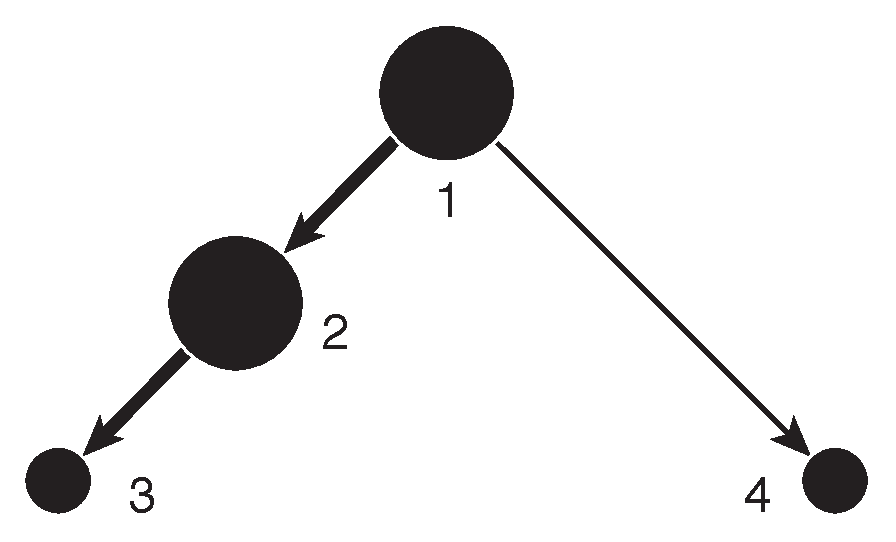
\includegraphics[scale=0.4]{mim/source_sink}
\end{center}
\caption{Source-sink example}\label{ss}
\end{figure}
Source-Sink (the first population is the source (Figure \ref{ss})):\\
{\bt{custom-migration=\{*000**000**0*00*\}}}

\subsection{Geographic distance between locations}
You can specify a distance matrix between your populations.
the distance file has the same syntax as a PHYLIP distance file [see example below].\\

{\bt{geofile=$<$NO $|$ YES:filename$>$}}\\
The distance matrix contains the distances between pairs of populations, if you choose
for example distance units in kilometers you will get migration rate estimates that are scaled
as M = immigration rate / (mutation * kilometer), if you restrict the migration rate to an average value
for all connections between population you are calculating a dispersion coefficient based on discrete
populations. This coefficient should be in the limit the same as the one calculated  from a isolation by distance population model.
\\ 
There is no requirement that the distances from i to j are the same as from j to i, although interpretation might be difficult with
an unequal distance matrix. the default filename for this distance file is \textsl{geofile}.

Example \textit{ geofile}\\
\begin{verbatim}
     3
Ermatingen0.0 10.4 12.4 
Schachen  10.4 0.0 1.0
Heiden    12.4 1.0 0.0
\end{verbatim}
\newpage
\section{Search strategy}
This section is the key to good results and you should not just use the defaults, for guidance how I myself would do this check out the section {\bt{how long to run}}.

\subsection{Maximum likelihood inference}
\begin{figure}[bh]

\begin{center}

\begin{boxedminipage}{6in}
\begin{small}
\ttfamily{
\begin{verbatim}
  SEARCH STRATEGY

  0   Strategy:                         Maximum Likelihood
  1   Number of short chains to run?                    10
  2   Short sampling increment?                         20
  3   Number of recorded genealogies in short chain?   500
  4   Number of long chains to run?                      3
  5   Long sampling increment?                          20
  6   Number of recorded genealogies in long chain?   5000
  7   Number of genealogies to discard at 
      the beginning of each chain? [Burn-in]         10000
  8   Combine chains or runs for estimates?             NO
  9   Heating:      YES (  4 chains, swap interval is   1)

 -------------------------------------------------------------
 Obscure options (consult the documentation on these)

 10   Sample at least a fraction of new genealogies?    NO
 11   Epsilon of parameter likelihood             infinity
 12   Use Gelman's convergence criterium?      YES:Summary


  Are the settings correct?
  (Type Y to go back to the main menu or the number for a menu to change)
===>
\end{verbatim}
}
\end{small}
\end{boxedminipage}
\end{center}
\caption{\textsf{ `Search strategy' menu with the Maxim likelihood approach}}
\label{SEARCHMA}
\end{figure}

\par
The terminology of {\bt{short}} or {\bt{long}} chains is arbitrary, actually
you could choose values so that short chains are longer than the ``long''
chains. Anyway, Markov chain Monte Carlo (MCMC) approaches tend 
to give better results when the start parameters are close to the maximum
likelihood values. One way to achieve this is running several short chains
and use the result of the last chain as starting value for the new chain.
This should produce better and better starting values, 
if the short chains are not too short. 

\begin{description}
\item{\bt{Strategy}}\\
With version 2.0 you have a choice of either using a maximum likelihood procedure or a Bayesian approach, on nice data both method will work about the same, for some example runs it seems that the profile likelihoods and the Bayesian posterior distribution agree quite fine on the distribution of the parameter value. The options specific to the Bayesian approach are explained in the next section.
\item{\bt{Number of short chains to run? (short-chains=value}}\\
we run most of the time about 10 short chains, which is enough if the
starting parameters are not too bad. Default is {\bt{short-chains=10}}.

\item{\bt{Short sampling increment? (short-inc=value)}}\\
The sampled genealogies are correlated to reduce the correlation between genealogies and to allow for a wider search of the genealogy space (better mixing), we sample not every genealogy, the default is {\bt{short-inc=20}}
means that we sample a genealogy and step through the next 19 and sample then
again.

\item{\bt{Number of steps along short chains? (short-steps=value)}}\\
The default number of genealogies to sample for short chains is 500.
But this may be to few genealogies for your problem. If you big data sets it
needs normally bigger samples or higher increments
to move around in the genealogy space.

\item{\bt{Number of long chains to run? (long-chains=value)}}\\
I run most of the time 3 long chains. The first equlibibrates and the last
is the one we use to estimate the parameters. Default is {\bt{long-chains=3}}.

\item{\bt{Long sampling increment? (long-inc=value)}}\\
The default is the same as for short chains. 

\item{\bt{Number of steps along long chains? (long-steps=value)}}\\
The default number of genealogies to sample for long chains is 5000.
I often choose the ``long'' chains about 10 times longer than the ``short`` chains.
\item{\bt{Number of genealogies to discard at the beginning of each chain?\\
(burn-in=value)}}\\
Each chain
inherits the last genealogy of the last run, which was created with the old parameter set. Therefore the first few genealogies are biased towards the old parameter set. When {\bt{burn-in}} is bigger than 0, the first few genealogies
in each chain are discarded. 
The default is {\bt{burn-in=10000}}.

\item\textbf{ Combine chains for estimates}
The use of this option is recommended for difficult
data sets. It allows to combine multiple chains for the parameter 
estimates when you use \textbf{ replicate=YES:LongChains}. 
With  \textbf{ replicate=YES:number} where number is, well, 
a number bigger than 1. (e.g. replicate=Yes:5), you run the program ``number'' times and the results of their last chains are combined,
The method of combination of chains is the same as in \cite{kuhner:1995:eep}
and is based on the work by \cite{geyer1991-t}. The LongChain option does not need much more time than the single chain option, but the full replication needs
exactly ``number'' times a normal run. But is sampling the search space
much better than any other option, I use this often in conjunction with
random starting trees (randomtree=YES). 
\item\textbf{ Heating (heating=$<$NO $|$ YES $|$ ADAPTIVE $<$:waitnumber:\{cold,warm,hot,boil,....\}$>$}\\
This allows for running multiple chains and swap between them, when 
these chains are run at different temperatures, 
the ``hotter'' chains explore more genealogy space than the 
``cold'' chains. An acceptance-rejection
step swaps between chains so that the the ``cold'' chains will sample
from peaks on the genealogy surface proportional to their
probability. This scheme is known as MCMCMC (Markov 
coupled Markov chain Monte Carlo),
it is based on the work of \cite{geyer:1995:amc} and uses for
four or more chains at different temperatures, the hotter chains move more freely
and so can explore other genealogies, this allows for an efficient 
exploration of data that could fit different genealogies, and should help
to set the confidence intervals more correctly than a single chain path 
could do. You need to set the temperatures yourself because there is no default.
The ADAPTIVE heating scheme manipulates these temperatures according to their
swapping success. If a neighboring temperature pair is not swapping after 1000 trials
the temperature difference between them is lowered by 10\%, if a pair is swapping more than
10 times in a 1000 the gap is increase by 10\% (these values are arbitrary, but cannot be changed in the menu, yet).
Adaptive heating is definitely no cure-it-all, I typically prefer the static heating, but it helps find good values to try for the static heating scheme, I have seen pathological behavior of long adaptive runs where all chains essentially converged to values very very close to 1.0 (the cold chain) and stopped swapping. 

If you use a STATIC heating scheme then you need to experiment a little because you want that the different
chains swap once in a while, but not too often and certainly more often
than never. The swapping seems to depend on how good the data describes a 
given genealogy. I would start with 4 chains and 
temperatures that are \textbf{ \{1. 1.5 3.0 10000.0\}}. 
The temperatures are ordered 
from cold to boiling, the coldest temperature \textbf{ MUST} be 1 (one).
The default for the heating option is \textbf{ heating=NO}. If you use
this option sampling will be at least 4 times slower, except 
if you have a multiprocessor machine and a POSIX compliant thread-library
(often called with slight variations but containing word parts such 
as pthread, thread, linuxthread), 
then you can compile the program using ``make thread'',  this will improve speed somewhat, but lately I do not gain more than 170\% CPU usage out of this. It is probably easier and faster to use all cores on new computers using the parallel version of \migrate.

The \textbf{ waitnumber} is the number of trees to wait before the differently heated chains are check whether to swap or not. I normally use 1. I have little experience whether, say, using 10 improves mixing over using 1.
\end{description}

\subsubsection{Obscure options}
If you are not experienced with MCMC or run \textit{ Migrate} for the first, 
second, ... time, do not bother about the options here.
\begin{description}
\item{\bt{Sample at least a fraction of new genealogies? ( moving-steps=$<$Yes:ratio $|$ No $>$)}}\\
With some data the acceptance ratio is very low, for example with 
sequence data with more than 5000 bp the accpetance ratio drops below 10\%
and one should increase the length of the chains. One can do this either by increasing the {\bt{long-inc}}, or {\bt{long-steps}} or by using
{\bt{moving-steps}}. The ratio means that at least that ratio of genealogies
specified in {\bt{long-steps}} have to be  new genealogies and if that fraction
is not yet reached the sampler keeps on sampling trees. In unfortunate situation this can go on for a rather long period of time.
You should always try first with the default {\bt{moving-steps=No}}.
An example:\\
You specified {\bt{long-steps=2000}},and {\bt{long-inc=20}} and the acceptance-ratio was only 0.02, you have visited 40,000 genealogies of which only 800 are new genealogies so that you have maximally sampled 800 different
genealogies for the paramter estimation.
In a new run you can try {\bt{moving-steps=Yes:0.1}}, the sampler is now extending the sampling beyond the 40000 genealogies and finally stopping when 4000 new genealogies were visited.

\item{\bt{Epsilon of parameter likelihood (long-chain-epsilon=value)}}\\
The likelihood values are ratios
\begin{align}
\frac{L(\P)}{L(\P_0)}&=\frac{1}{n} \sum_i\frac{\prob(G_i | \P)} {\prob(G_i | \P_0)}\qquad\text{(Beerli and Felsenstein, 1999)}\nonumber
\end{align}
When the Likelihood values are very similar then the ratio will be close
to 1, or 0 when we use logarithms. This means that the sampler
is not improving drastically between chains: (a) it found the maximum likelihood estimate or (b) it is so far from the maximum likelihood estimate that the surface is so flat that all likelihood values are equally bad.
using a smaller value than the default {\bt{long-chain-epsilon=100.00}}
for example a value of 1.0 would guarantee that the sampler keeps on 
sampling new long chains as long as that log-likelihood-difference drops below 1.0. In some cases this will never happen and the program will not stop.
\item{ \textbf{Gelman's convergence criterium}} If you specify ``Yes'' then 
the number of last chains get extended until the convergence criterium
of Gelman is satisfied (the ratio should be smaller than 1.2 for \textbf{ all} parameters. This can take a very long time. [In the parallel version this fails, turn it off there [this is a bug, but I had not time to find and fix it]).
\end{description}

\subsection{Bayesian method}
\begin{figure}[bht]

\begin{center}

\begin{boxedminipage}{6in}
\begin{small}
\ttfamily{
\begin{verbatim}
 SEARCH STRATEGY

   0   Strategy:                                    Bayesian Inference
   1   File for recording posterior distribution?                   NO
   2   File for recording all parameter values?                     NO
   3   Number of bins of posterior [Theta,M]?                 200, 200
   4   Plotting type of posterior distribution? up to ~100% percentile
   5   Frequency of tree updates vs. parameter updates?           0.50
   6   Proposal distribution?         Theta:Slice Mig:Slice Rate:Slice
   7   Prior distribution?            Theta:Unif. Mig:Unif. Rate:Unif.
   8   Number of long chains to run?                                 1
   9   Sampling increment?                                          20
  10   Number of recorded steps in chain                          5000
  11   Number of steps to discard at 
       the beginning of chain? [Burn-in]                         10000
  12   Running multiple replicates:                                 NO
  13   Heating:                           STATIC (  4 parallel chains)
  14   Sampling at least fraction of new genealogies:         0.000000
  15   Convergence diagnostic for replicates:              YES:Summary


  Are the settings correct?
  (Type Y to go back to the main menu or the number for a menu to change)
===>
\end{verbatim}
}
\end{small}
\end{boxedminipage}
\end{center}
\caption{\textsf{ `Search strategy' menu with the Bayesian approach}}
\label{SEARCHBA}
\end{figure}
\begin{description}
\item{\bt{File for recording parameters? (bayesfile=$<$NO $|$ YES:bayesfile$>$)}} 
this file contains the raw histogram for all parameters and all loci and their combination, figure \ref{BAYESFILE} shows the first few lines of an example, see under section \textbf{Bayesian posterior explained} further uses of this file.
\begin{figure}[bht]

\begin{center}

\begin{boxedminipage}{6in}
\begin{small}
\ttfamily{
\begin{verbatim}
# Raw data for the histogram of the posterior probabilities for all parameters
# and loci  produced by the program migrate-n 2.0.3 
# (http://evolution.gs.washington.edu/lamarc/migrate.hml)
# written by Peter Beerli 2004, Tallahassee, 
# if you have problems email to beerli@csit.fsu.edu
#
# The HPC values are indicators whether the parametervalue is in the 
# highest-posterior credibility set, a 0 means it is outside and a 1 means 
# the value is inside the credibility set.
#
# Delta for Theta and M 0.001000 0.001000 9.995000 9.995000 
# ----------------------------------------------------------------
# Locus Parameter 50%HPC  95%HPC (parameter-value count) frequency
# ----------------------------------------------------------------
1 1 0 0 0.002499 327 0.001635
1 1 0 0 0.003498 1634 0.008169
1 1 0 1 0.004498 4612 0.023058
1 1 0 1 0.005497 8970 0.044846
1 1 1 1 0.006497 13576 0.067874
1 1 1 1 0.007496 17320 0.086592
1 1 1 1 0.008496 19492 0.097451
1 1 1 1 0.009495 20537 0.102676
1 1 1 1 0.010495 19504 0.097511
\end{verbatim}
}
\end{small}
\end{boxedminipage}
\end{center}
\caption{\textsf{ First few lines of a bayesfile: the header explains the columns}}
\label{BAYESFILE}
\end{figure}

\item{\bt{File for recording all parameter values? (bayes-allfile=$<$NO $|$ YES:number:bayesallfile$>$)}}
this file contains the raw histogram for all parameters and all loci and their combination, figure \ref{BAYESALLFILE} shows the first few lines of an example, see under section \textbf{Bayesian posterior explained} for further uses of this file. This file can be very large depending on your options, it is still hard to work with files larger than 10 GB, so choose you settings carefully, there will be samples$\times$loci$\times$replicates sets of $n^2$ parameters and some additional values. If you need more samples to get good results and your data is highly autocorrelated increase the long-inc options (see there). If you specify this option (recommended) the memory foot print of the program is smaller than when this option is set to NO. This is important particularly for the parallel \migrate runs.

\begin{figure}[bht]

\begin{center}

\begin{boxedminipage}{6in}
\begin{tiny}
\ttfamily{
\begin{verbatim}
# Migrate debug 3.0 (Peter Beerli, (c) 2008)
# Raw results from Bayesian inference: these values can be used to generate
# joint posterior distribution of any parameter combination
# Writing information on parameters (Thetas, M or xNm)
# every 2 parameter-steps
# 
# --  Steps
# --  Locus
# --  Replicates
# --  log(Posterior)
# --  log(prob(D|G))
# --  log(prob(G|Model))
# --  log(prob(Model))
# --  Sum of time intervals on G
# --  Total tree length of G
# Order of the parameters:
# Parameter-number Parameter
#@      1    Theta_1
#@      2    Theta_2
#@      3    M_(2,1)
#@      4    M_(1,2)
# 
# --  Thermodynamic temperature = 1.000000
# --  Thermodynamic temperature = 1.500000
# --  Thermodynamic temperature = 3.000000
# --  Thermodynamic temperature = 1000000.000000
# --  Marginal log(likelihood) [Thermodynamic integration]
# --  Marginal log(likelihood) [Harmonic mean]
# 
#$ ------------------------------------------------------------------ 
#$ begin  [do not change this content]
#$ Model=****
#$ Mode2=****
#$ 1 2 4 0 1 1
#$ pop00
#$ pop01
#$ end
#$ ------------------------------------------------------------------ 
# 
# remove the lines above and including @@@@@, this allows to use
# Tracer (http://tree.bio.ed.ac.uk/software/tracer/) to inspect
# this file. But be aware that the current Tracer program (October 2006)
# only works with single-locus, single-replicate files
# The migrate contribution folder contains a command line utility written
# in PERL to split the file for Tracer, it's name is mba
# @@@@@@@@
#Steps  Locus   Replicate       lnPost  lnDataL lnPrbGParam     lnPrior treeintervals   treelength      Theta_1 Theta_2 M_2_1   M_1_2
100     1       1       -22365.119577   -22620.671234   255.551656      -17.034386      95      0.092424        0.00449 ...
200     1       1       -22367.961876   -22622.328216   254.366340      -17.034386      95      0.093002        0.00379 ...
300     1       1       -22368.867271   -22618.681322   249.814051      -17.034386      95      0.092687        0.00460 ...
\end{verbatim}
}
\end{tiny}
\end{boxedminipage}
\end{center}
\caption{\textsf{ First few lines of a bayesallfile: the header explains the columns, the data section is truncated at the right and bottom}}
\label{BAYESALLFILE}
\end{figure}

\item{\bt{Number of bins of posterior (\textbf{ bayes-posteriorbins=$<$thetabins Mbins $<$ratebins$>$$>$)}}}\\
The number of bins for the posterior needs to be pre-specified (to save memory). The default for $\Theta$, $M$ is 200 bins.
This number is probably to small if the range of the prior distribution is very large. If the PDF histograms look course rerun after increasing the binsizes. The ratebins are used when the mutation rate modifier with many loci is estimated in the Bayesian analysis,
this may sometimes fail, because there is little information about rate differences among loci in some datasets.

\item{\bt{Plotting bins of posterior (\textbf{ bayes-posteriormaxtype=$<$TOTAL $|$ P100$|$ P99$|$ MAXP99 $>$)}}}\\
The posterior distribution often covers only a short range of the prior distribution, therefore displaying the \textbf{ TOTAL} range of the prior distribution is often not advised, the P99 presents 99\% of the posterior distribution, cutting of 1\% of the posterior, this is a good way to visualize posterior distributions with very long (thin) right tails. P100 takes 99.99\% of the values and excludes strange outliers. MAXP99 is cutting of at 99\% credibility, but using the parameter with the highest value  for $\Theta$, and $M$, in principle this forces the same scale in the output for the parameters (this needs more testing because I most often use P100).

\item\textbf{ Frequency of tree updates versus parameter updates  (bayes-updatefreq=$<$ value $>$)}\\
The \textsl{value} specifies the ratio of genealogy updates and parameter updates, 0.5 means that the genealogy is updated roughly every second time, and one of the parameters is updated every second time. A value of 1.0 means that the parameters are never updated, A value of 0.0 is not advised because the genealogy does not adjust the migration events and so does not really test the parameter distribution for a specific tree.

\item\textbf{ Proposal distribution\\
 bayes-posterior=$<$ $<$ THETA $|$ MIG $|$ RATE $>$ $<$ SLICE $|$ METROPOLIS $>$ $>$)}\\
There are two ways the generate posterior distributions: SLICE and METROPOLIS. METROPOLIS is using the standard Metropolis-Hastings algorithm that proposes a new state not taking into account the data and then accepting or rejecting using the fit if the data to the old and new state. For some data the rejection rate is very high and many computer cycles are wasted because the MCMC chain does not move. SLICE sampling uses the current posterior distribution (taking into account the data) to generate a new state, every new state is compatible with the data, therefore the acceptance ratio is always 1.0. This comes at a price because the calculations are more demanding than the MH algorithm, and therefore may be slower. On data with lots of information SLICE sampling is great, but fails with poor data.
SLICE is the default in \migrate.
\vskip 0.5cm
Examples:\begin{small}
\begin{verbatim}
bayes-proposals= THETA SLICE Sampler
bayes-proposals= MIG SLICE Sampler
bayes-proposals= RATE SLICE Sampler
\end{verbatim}
\end{small}

\item\textbf{ Prior distribution\\
 bayes-priors=$<$ $<$ THETA $|$ MIG $|$ RATE $>$ $<$ PRIORSPECIFICATION $>$ $>$)}\\
There are several prior distribution available, but the list is still short. 
For each prior distribution you need to specify additional parameters:

\begin{tabular}{l c c c c}
Distribution & parameter 1 & parameter 2 & parameter 3 & parameter 4\\
\hline
Uniform & Minimum & Maximum & Window size & -\\
Exponential & Minimum & Mean & Maximum & -\\
Windowed Exponential & Minimum & Mean & Maximum & Window size\\
\hline
\end{tabular}
\vskip 0.5cm
Examples:\begin{small}
\vskip -0.5cm
\begin{verbatim}
bayes-priors= THETA EXPPRIOR: 0.000000 0.250000 0.500000 
bayes-priors= MIG WEXPPRIOR: 0.000000 500.000000 1000.000000 100.000000 
bayes-priors= RATE UNIFORMPRIOR: 0.010000 100.000000 5.000000 
\end{verbatim}
\end{small}
\item{\bt{Number of long chains to run? (\textbf{ long-chains=$<$value$>$)}}}\\
Use 1 long chain because multiple long chains will do little to help the analysis, if you want to combine over replicated runs use the replicate option.

\item{\bt{Sampling increment? (\textbf{ long-inc=$<$value$>$)}}}\\
Samples are taken every  \textsl{value} cycle, the default is 20. 

\item{\bt{Number of recorded genealogies in chains? (long-steps=value)}}\\
The default number of genealogies to sample for long chains is 50000. With the default increment this means
1,000,000 genealogies will be visited
This is short for many datasets.
\item{\bt{Number of genealogies to discard at the beginning of each chain?\\
(burn-in=value)}}\\
The chain is not equilibrated at the beginning of the run, and we discard those aberrant values and trees. The default is {\bt{burn-in=10000}}.

\item\textbf{ Combine chains for estimates}
The use of this option is recommended for difficult
data sets. It allows to combine multiple chains for the parameter 
estimates when you use \textbf{ replicate=YES:number}; where the number is bigger than 1. (e.g. replicate=Yes:5). 
You run the program ``number'' times and the results are combined (similar to MrBayes).
The option  \textbf{ replicate=YES:number} works for both Bayesian inference and Maximum Likelihood. The work is number times more than without replication.
For ML there is another option:  \textbf{ replicate=YES:LongChains} that allows the combination of long chains only, this is the same method as used by  \cite{kuhner:1995:eep} and is based on the work by \cite{geyer1991-t}. The LongChain option does not need much more time than the single chain option.

Replication allows a better sampling of the search space than the single chain. in particular when used on parallel cluster computers. I use this often in conjunction with random starting trees (randomtree=YES). 

\item\textbf{ Heating  (heating=$<$NO $|$ YES $|$ ADAPTIVE $<$:waitnumber:\{cold,warm,hot,boil,....\}$>$}\\
This allows for running multiple chains and swap between them, when 
these chains are run at different temperatures, 
the ``hotter'' chains explore more genealogy space than the 
``cold'' chains. An acceptance-rejection
step swaps between chains so that the the ``cold'' chains will sample
from peaks on the genealogy surface proportional to their
probability. This scheme is known as MCMCMC (Markov 
coupled Markov chain Monte Carlo),
it is based on the work of \cite{geyer:1995:amc} and uses for
four or more chains at different temperatures, the hotter chains move more freely
and so can explore other genealogies, this allows for an efficient 
exploration of data that could fit different genealogies, and should help
to set the confidence intervals more correctly than a single chain path 
could do. You need to set the temperatures yourself because there is no default.
The ADAPTIVE heating scheme manipulates these temperatures according to their
swapping success. If a neighboring temperature pair is not swapping after 1000 trials
the temperature difference between them is lowered by 10\%, if a pair is swapping more than
10 times in a 1000 the gap is increase by 10\% (these values are arbitrary, but cannot be changed in the menu, yet).
Adaptive heating is definitely no cure-it-all, I typically prefer the static heating, but it helps find good values to try for the static heating scheme, I have seen pathological behavior of long adaptive runs where all chains essentially converged to values very very close to 1.0 (the cold chain) and stopped swapping. 

If you use a STATIC heating scheme then you need to experiment a little because you want that the different
chains swap once in a while, but not too often and certainly more often
than never. The swapping seems to depend on how good the data describes a 
given genealogy. I would start with 4 chains and 
temperatures that are \textbf{ \{1. 1.5 3.0 10000.0\}}. 
The temperatures are ordered 
from cold to boiling, the coldest temperature \textbf{ MUST} be 1 (one).
The default for the heating option is \textbf{ heating=NO}. If you use
this option sampling will be at least 4 times slower, except 
if you have a multiprocessor machine and a POSIX compliant thread-library
(often called with slight variations but containing word parts such 
as pthread, thread, linuxthread), 
then you can compile the program using ``make thread'',  this will improve speed somewhat, but lately I do not gain more than 170\% CPU usage out of this. It is probably easier and faster to use all cores on new computers using the parallel version of \migrate.

The \textbf{ waitnumber} is the number of trees to wait before the differently heated chains are check whether to swap or not. I normally use 1. I have little experience whether, say, using 10 improves mixing over using 1.

\item{\textbf{Sampling at least fraction of new genealogies (moving-steps=$<$NO $|$ YES:value $>$)}}
This allows to specify that a minimum number of different genealogies need to be sampled, it is expressed as the ratio of sampled genealogies. If the frequency is not reached at the end of the specified number of samples, \migrate will continue until the ratio is satisfied, with high numbers the program may run forever. I rarely use this option.
 
\item{ \textbf{Convergence diagnostic for replicates (gelman-convergence=$<$ NO $|$ YES:$<$Sum $|$ Pairs $>$ $>$}}
This collects information about the convergence rate of two replicated chains (use two or more replicates). \textsl{Sum} reports the an average value over all whereas \textsl{Pairs} using the pairs of replicates to. Version 3.0 has some difficulties with this option and I hope to fix this in the next minor release, but on some machine and under some conditions the diagnostic fails.
 
\end{description}
%%%%%%%%%%%%%%%%%%
\subsection{Parmfile specific commands}
\subsubsection{Important parmfile options}
\begin{description}
\item{\bt{menu=$<$Yes$|$No$>$}}\\
defines if the program should show up the menu or not.
The default is {\bt{menu=Yes}}.

\item{\bt{end}}\\
Tells the parmfile reader that it is at the end of the parmfile.
\end{description}

\subsubsection{Options to change the lengths of words and texts}
If you change these, you should understand why you want to do this.
\begin{description}

\item{\bt{nmlength=number}}\\
defines the maximal length of the name of an individuum, if for a strange
reason you need longer names than 10 characters (e.g. you need more than
10 chars to characterize an individual) and you do not need this
very often then set it to a higher value, if you have no individual names
you can set this to zero (0) and no Individual names are read.
the default is {\bt{nmlength=10}}, this is the same as in PHYLIP.

\item{\bt{popnmlength=number}}\\
Is the length of the name for the population.
The default is {\bt{popnmlength=100}}

\item{\bt{allelenmlength=number}}\\
This is only used in the infinite allele case.
Length of an allele name, the default should cover even strange
lab-jargons like \texttt{ Rvf} or \texttt{ sahss} (\textit{ Rana ridibunda} very fast, \textit{ Rana saharica} super slow)
The default is {\bt{allelenmlength=6}}
\end{description}
\end{description}
% !TEX root = migratedoc.tex
\chapter{How to run \migrate}
If you have compiled and installed the program successfully (see Installation) and your data is in a good format (section data format) and perhaps has the name infile, just execute
\smallerskip
\begin{tabular}{l l p{10cm}}
Command & Parameters & Comments\\
\hline
\texttt{ migrate-n} &  & No option will take the default \texttt{ parmfile} if present\\
\texttt{ migrate-n} &  parmfile.test & opens the file \texttt{ parmfile.test} if present otherwise creates a new file that can be save through the menu\\
\texttt{ migrate-n} &  parmfile.test -menu & forces the program to show the menu\\
\texttt{ migrate-n} &  parmfile.test -nomenu & forces the program to NOT show the menu and start running immediately (use the -nomenu option for batch scripts and batch queue system.
\end{tabular}

On some systems you need to call \migrate using \texttt{ ./migrate-n}.

\smallerskip
On most graphical systems you can start \migrate by double-clicking its icon, but the results are different among the different computer systems (Linux, MacOS 10, Windows). On Macs home directory and that is most likely not the location where your files sit. It is actually easier to open the Terminal.app (in /Applications/Utilities) and 
learn a couple of shell commands (a minimal set of cd, mv, cp will probably do for a start) (see for example this online tutorial http: ). Within the terminal window you change to the directory with the data and then execute the program that either is in the same folder using the commands above. For windows double-clicking opens also a terminal window that is located at the same directory location as the icon, if your data is also in that same location your are set, but you can use the ``Run..." command from the Startup menu to open a terminal window and then use chdir, copy, rename to operate the windows shell similarly to the UNIC shell.

Without any \textbf{ parmfile}, \textit{ Migrate} will display a menu, in which you can change all the sensible options. For hints how to use the parmfile, look into section \textbf{ Menu and Options} or the \texttt{ parmfile}. Once you know how to customize the options with the \textbf{ parmfile} you will probably more often
edit the parmfile than making the changes in the menu. Be careful, some complex options are most easily set through the menu.





\chapter{Bayesian inference}
From a practical viewpoint we can think of Bayesian inference of a combination of knowledge: the prior knowledge and the knowledge gained through the data and model.  The prior knowledge is used to to treat the parameters of interests as random variables with a distribution that is typically independent of our investigation, the prior distribution. The posterior distribution is the product of the prior distribution and the probability of the data given the parameters (the likelihood). 
The prior distribution needs to cover the interesting part of the range of the parameters, essentially the posterior distribution should fit within the range of the prior distribution. It is important to inspect the posterior for probably truncation by the prior, if that occurs ou should rerun the analysis. If the prior is much larger than the parameter region of interest, in many circumstances the analysis will take a long time because most values proposed from the prior do not fit well with the data and are rejected. 
%(see Figure \ref{bayes}}
%\begin{figure}
%\begin{center}
%\includegraphics[width=\textwidth]{mim/bayes}
%\caption{Prior distribution affects the posterior distribution:(a) the prior is not covering the interesting range, (b) good prior, (c) the prior is weak, (d) the prior is very strong}
%\label{bayes}
%\end{center}
%\end{figure}

\section{Prior distribution}
Currently there are three distributions available: uniform, exponential  with boundaries, 
exponential with boundaries and windowing:
\begin{description}
  \item[Uniform prior] You need to specify a lower and an upper bound, this prior distribution is similar to other programs, such as those by Hey and Nielsen (2004). Uniform assume that all parameter values are equally likely, an assumptions that often is not justified. 
  \item[Exponential prior with boundaries] This proper prior distribution (it integrates to 1) needs a lower and and an upper bound and a mean, if one specifies $0.0$ and $\infty$ as boundaries, this distribution is the same as a simple exponential distribution. Preliminary runs show that this distribution is superior (aka converges faster) than the uniform distribution prior. Typically the boundaries are chosen so that there is a large set of possible values in between, the method is picking randomly in this range and so from one step to the next large differences in parameter values can occur, this large differences might lead to a larger rejection rate.
  \item[Exponential prior with boundaries and window] Same as exponential prior with boundaries except that you need to specify an additional parameter that specifies the window size in from which changes in parameters are drawn. The chain will  less often reject parameter values because they will be closer to the last value. This prior distribution seems to produce the best results so far, but it needs some fidgeting with the window. If the window is too small very long chains need to be run to explore the whole distribution, if the window is too large than the method reduces to the exponential prior with boundaries. 
\end{description}

\section{Proposal distribution: Slice sampling versus Metropolis-Hastings sampling}
\migrate allows to use two different proposal functions for the evaluation of the parameters, but only one for the evaulation of genealogies: Metropolis-Hastings sampling \cite{metropolis:1953:ESC} and Slice sampling \citep{Neal:2003}. Metropolis-Hastings (MH) sampling is standard in most applications in population genetics, but Slice-sampling is not. I know that Paul Lewis (University of Connecticut) is working on a phylogeny program that uses slice-sampling but I have not see the program in the wild. Paul helped me to understand the slice-sampling method in 2006 at the molecular evolution workshop in Woods Hole.
Slice sampling uses the data and the prior distribution to choose a new prior value, because the data already is comaptibel with this new value a MH-rejection step is not necessary and the new value is always accepted. In contrast to that, MH-sampling picks a value from the prior and then uses the data later in the rejection-acceptance step to accept or reject the new value. Experiments have shown that slice-sampling converges  typically faster and produces smoother posterior distributions with less steps on the MCMC chain.

\section{Posterior distribution}
\migrate\ prints a file \textsl{bayesfile} that contains the raw histogram values for all parameters, the columns in that file allow to use  graphing program such as GNUPlot (http://www.gnuplot.info/) to plot the distribution. My favored program to plot such graphs is GMT (General mapping tool, http://gmt.soest.hawaii.edu/) that produces postscript output, in the contribution directory I added a shell script
(sorry, no MS Windows utility) that uses GMT and that produces posterior distributions that display the 95\% credibility set. 

\migrate also allows to save the raw parameter values that are used for the posterior distribution (\textsl{bayesallfile}). This file contains all information necessary to recreate the posterior histograms from scratch, This file also is compatible with the program \tracer \citep{Rambaut:2007} when you analyze a single locus without replication. There is a command line utility in the contribution directory. This utility \textsl{mba} allows to separate the large bayesallfile into files per locus and replicates. It also allows the assembly of different files, that can then be feed back to \migrate to recreate the posterior histograms.
If you run \migrate on a cluster in parallel use turn on this option because the memory footprint of \migrate is much smaller than when this option is turned off. 

\section{Prior distributions: choice and problems}
to come

%\chapter{Likelihood ratio tests and profile likelihood}
\subsection{Likelihood ratio test} 
The parameter estimation is done with  a maximum likelihood method, 
this gives the 
opportunity to easily test different hypotheses against others, when the hypotheses are hierarchical (e.g. Casella and Berger 1996). For example,
we wish to test if the migration rates are the same 
in a two population model with 4 parameters: 
\begin{align}
H_0:& \M_{21} = \M_{12}\qquad \Theta_1 = {\hat \Theta_1},\Theta_2 = {\hat \Theta_2},\\
H_1:& \M_{21} \neq \M_{12}\qquad \Theta_1 = {\hat \Theta_1},\Theta_2 = {\hat \Theta_2},\\
\intertext{and then can test using the test statistics}
-2& \log\left(\frac{{\rm L}(\Theta_x)}{{\rm L}(\hat\Theta)}\right) \le \chi^2_{df,\alpha}\label{LRATIOFORM}
\end{align}
In the example the degrees of freedom would be two: we are 
changing two parameters.
We need to run {\tt migrate} with the full model: all parameter can vary
independently. We get parameter estimates ${\hat \Theta_1}$, ${\hat \Theta_2}$,
${\hat \M_{21}}$, and ${\hat \M_{12}}$. We compare this maximum likelihood
with the likelihood when we restrict the migration rate to be the same
for example the mean of both estimates. The ratio between these two likelihoods
is in the limit (if there is a huge amount of data) $\chi^2$ distributed 
(Formula \ref{LRATIOFORM}, Figure \ref{LRATIOFIG}). 
If the probability is smaller than $0.05$ we would reject the 
Null-hypothesis and accept the alternative, saying that the values
are not equal.
If you have mtDNA data this methods is theoretically not applicable, because
you cannot increase the data beyond the full sequence of the mitochondrion,
but I am pretty sure that for most situations the test will 
still work. 
There is a problem due to the implementation of the program that we can
not allow that parameters go to 0.0. A parameter of 0.0 has a 0.0 probability. 
we would need to correct for the fact that our parameter might be on the boundary of its range.
If we assume that the parameters are independent then under some conditions we can calculate 
a test statistic that takes this boundary condition into account [but this is not yet yet implemented in the
l-ratio test]. If you test just if a single parameter is 0.0 then the test needs a halved significance level (cit).
\begin{figure}[htb]
\begin{center}
\leavevmode
\hbox{%
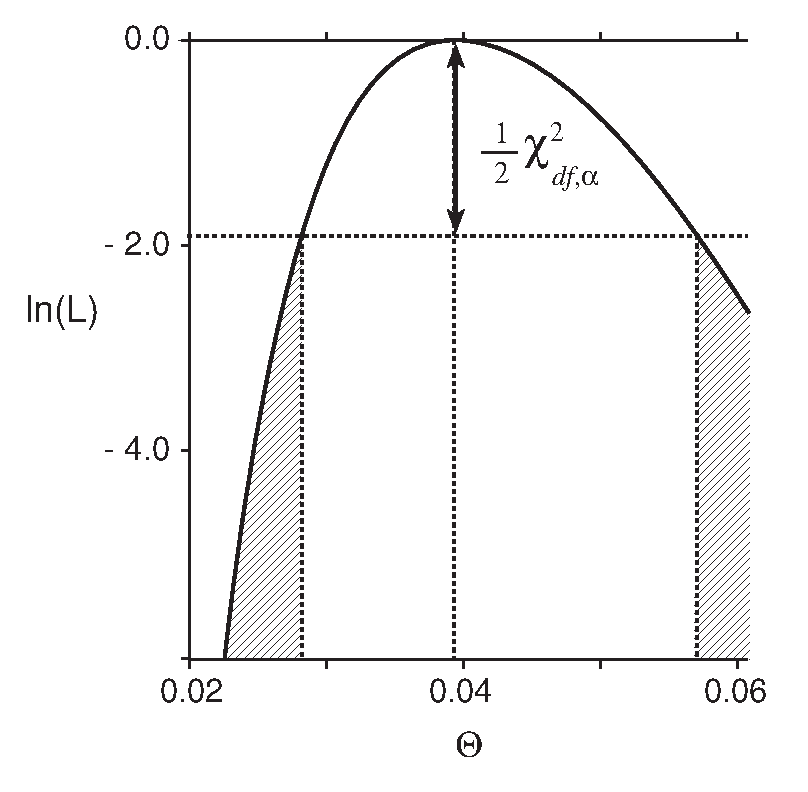
\includegraphics[scale=0.6]{mim/coalesce_likecurve}}
\end{center}
\caption{Likelihood ratio test: dashed areas are outside of the 95\% confidence limit. $\Theta$ is $4 N_e \mu$; $df=1$, $\alpha=0.05$ \label{LRATIOFIG}}
\end{figure}

Do not forget that these likelihoods are only 
approximations. Comparison with exact likelihoods for
genealogies with 3 tips and no migration show that the MCMC curves are
exactly the same as the ``exact'' curves. When the program is not run long 
enough the MCMC curves tend to be wider than the ``exact'' curves and 
have their maximum biased towards the parameter value at which we run the chains. We expect
when there are many sampled individuals that it is likely that you
run the program not long enough and therefore will get wrong confidence
interval estimates and will stick too close to the start parameters.
(Figure \ref{EXACT_MCMC}). 
You can check for this by running the program several
times from very different start values. Just looking at the point estimates
is probably not enough, you should to inspect the profile likelihoods, too.
Most of the time it seems that real single locus data is not very great for
the estimation of migration rates and the ``confidence'' intervals are huge. 
\begin{figure}[htb]
\begin{center}
\leavevmode
\hbox{%

\includegraphics[scale=0.6]{mim/exact_and_mcmc}}
\end{center}
\caption{Log likelihood curves from (a) the exact likelihood 
calculation for a genealogy with 3 samples, (b) an MCMC based estimator
with only one (1) sampled genealogy with start value $\Theta_0=\text{Watterson estimate}$, 
(c) with one acceptance using a $\Theta_0=0.00001$. The data are 3 sequences each
1000 bp long and generated with a $\Theta=0.1$, running the program some 1000
genealogies delivers a likelihood curve indistinguishable from the exact likelihood curve.
\label{EXACT_MCMC}}
\end{figure}

For the {\tt parmfile} there is an option {\bt{l-ratio}} which you can use to 
define a hypothesis against the program run (Null-hypothesis). 
You can repeat the statement for testing more than one hypothesis,
but you may need to correct your significance level for multiple tests. 
The syntax is:\\
{\bt{l-ratio:$<$YES$>$ $<$:param1,param2,param3,....paramn*n$>$}}\\
\begin{description}
\item{\bt{Means}} over all loci
\end{description}
The syntax for each {\bt{param1, param2,...}} is rather complicated:
{\bt{param1 = $<$* $|$x $|$  m $|$ value$>$}}\\
\begin{description}
\item{\bt{*}} the value is the same as the one from the estimate ($=H_1$)
\item{\bt{x}} the value will be maximized.
\item{\bt{m}} the value is the mean of the parameters, either $\Theta$ or $\M$.
\item{\bt{s}} the parameters is symmetric in $\M$.
\item{\bt{S}} the parameter is symmetric in $\Theta\M= hN_em$ (h is the inheritance factor: 4 for diploids, 2 for haploids, 1 for haploids passed on by one sex).
\item{\bt{value}} is any arbitrary value you want to test.
\end{description}
Examples for two populations for the parmfile entries:\\
{\bt{l-ration=YES:0.01,1.0,1.1,0.011;\\
l-ratio=YES:*,m,m,*;\\
l-ratio=YES:x,1.34,*,0;
}}
\smallskip%\multicolumn{1}{c}{
For the test you need to to specify the migration matrix with $\Theta$ values on the diagonal.
The parameters are ordered like this:\\
\begin{tabular}{ccccc}
$\Theta_1$, & $\M_{2,1}$,& $\M_{3,1}$,& ...,& $\M_{n,1}$,\\
$\M_{1,2}$,& $\Theta_2$,&  $\M_{3,2}$,& ...,& $\M_{n,2}$, \\
\multicolumn{5}{c}{...}\\
\multicolumn{3}{c}{...}& $\M_{(n-1),n}$,& $\Theta_n$
\end{tabular}

The calculations are always done using the scaled migration rate $\M$ but are adjusted according to the options and might print out hNm.\medskip
Example with 3 populations based on the following migration matrix:
\begin{gather}
\begin{matrix}
- &2&1\\
1.8&-&1\\
0.5&0.6&-
\end{matrix} \nonumber
\end{gather}
results in the string\\
{\bt{l-ratio=YES:*, 2,1,1.8,*,1,0.5,0.6,*;}}

Do not forget the semicolon at the end [ a comma will do too, but NO comma or semi-colon might fail].
\newpage
\section{Profile likelihood}
Parameter estimation in high dimensions causes serious problems 
in the presentation of results: for 2 population we have 4 parameters,
with 8 population 64, etc. One would like to show the high dimensional surface
but we are crudely limited to 3 and perhaps can understand graphs up to five.
Showing one parameter at a time only shows us a transection through the solution space, but is perhaps the best we can do. By using profile likelihoods
we can trace a parameter and also see how the other parameter change at given 
values for our profile parameter. Instead of finding the parameters at the maximum likelihood, we fix the profile parameter at some arbitrary value and then maximize the other parameters at that profile likelihood. This constructs a path through the solution space, which we can use to construct approximate confidence limits
using the likelihood ratio test criteria (Fig \ref{PROFILEFIG}) with a degree of freedom of 1 (well, this is true in ``asymptopia'' 
but may produce very tight confidence intervals \cite{beerli:2001:mle}. Several advanced statistic textbooks discuss the use of likelihood ratio and
the related profile likelihoods \cite[e.g. ][]{casella:1996}, but I like the compact,
and in my opinion, very readable, short text of \cite{meeker:1995:taa}. 
 
\begin{figure}[htb]
\begin{center}
\leavevmode
\hbox{%
\includegraphics[scale=0.6]{mim/profile_real}}% profile.example
\end{center}
\caption{{Profile likelihood, for a series of values of a parameter, the other parameter are maximized and the likelihood given that parameter is highest along the straight lines in A. (A) Contour plots for a run with two variables,
the thick lines are the 50\%, 95\%, and 99\% confidence contours. (B) is the
profile likelihood curve for $\Theta$ and (C) is the profile likelihood curve
for 4Nm (based on $\M$). The 95\% confidence range for B and C are for values 
with log likelihood values above -2.} 
\label{PROFILEFIG}}
\end{figure}

%\caption{Profile likelihood, for a series of values of a parameter, the other parameter are maximized and the likelihood given that parameter is highest along the thick line. The contours are approximate confidence areas based on the likelihood ratio test. The star is the maximum likelihood estimate for all
%parameters}
\newpage
\chapter{Model selection}
[This section is not finished] \migrate allows to calculate the probability of the model using three approaches:
\begin{enumerate}
  \item Akaike's information criterion (AIC) for maximum likelihood inference
 An option the parmfile allows to turn on a search for all migration model that are subsets of the model that was used to sample genealogies [this may break on several models with low number of estimated parameters]. 
This option may use a very long time (longer than you want to wait) when there are more than 4 (!) populations. The number of migration models increases hyper-exponentially with number of populations, AIC tests with more than 6 populations will take forever. These tests are only approximate because only the full model was evaluated through the MCMC run. 
% \begin{small}
% \begin{verbatim}
% insert example
% \end{verbatim}
% \end{small} 
 
  \item Bayes factors
  Bayes factors evaluate the merit of hypotheses and models in a Bayesian context. BF do not need to compare nested hypotheses (necessary for likelihood ratio tests). Evaluating Bayes factors is problematic because the marginal likelihoods needed to calculate the BF are difficult to evaluate. In a Bayesian inference program we normal only need to record the parameter values to construct the posterior distribution (histogram). For the marginal likelihood we need to estimate the denominator of the Bayes formula, we can integrate by recording all priors and likelihoods. Two methods are implemented in MIGRATE:
 \begin{enumerate}
  \item Harmonic mean estimator: described by Kass and Raftery (1996) . This method is know to be fast but inaccurate. It is implemented in many other programs (BEAST/Tracer, MrBayes)
  \item Thermodynamic integration: described by Gelman and Meng (2003). This method needs multiple chains that run at different temperatures (use static heating because the other methods are not well explored yet). This methods can be very accurte but time consuming.
\end{enumerate}
\end{enumerate}

\chapter{Performance of  \migrate}
\myabstract{Markov chain Monte Carlo programs are difficult to use and despite what people tell you very error-prone. This chapter tries to convince you that \migrate often is doing the correct thing, and when something goes wrong that you perhaps can find out why and how it went wrong.}

Markov chain Monte Carlo samplers have the proven property that when they are run infinitely long they converge to the correct value, but since we cannot run the program infinitely long, we are interested how many samples we need to get before we start to get ``acurate" result.  This is true for maximum likelihood and Bayesian inference modes of the program.
Despite the huge literature about measures when to stop sampling, there
is still no good universal criteria available. \migrate reports some measures, such as the effective sample size of an MCMC run, or the Gelman-Rubin statistic. The problem of difficulty to converge can be divided into three simple categories: 
\begin{enumerate}
\item Programming errors, typically programs of this complexity will always contain some errors, programmers certainly try to make every effort to make sure that there are no errors in the main calculations, but testing is typically very difficult especially when interactions among multiple options, different hardware need to be tested. 
\item The sampler was not run long enough, this is data dependent and some general guidelines could be given, 
%NSF slant 1
but NSF panels do not seem too keen to fund projects that would do that. To my knowledge, no study has explored effects of sample size, sequence lengths/variability of sequence for more than a single population \citep{Pluzhnikov:1996, Felsenstein:2005, Carling:2007}. You have to explore this with your own data.
\item The assumptions of the model are not met, all data will violate some of the assumptions but typically the method is quite tolerant.
\end{enumerate}
I will discuss some ways to investigate these three sources of problems in the following paragraph, highlighting the potential source of error.

The program is sampling form the right distribution: 
running the sampler with no data (e.g. sequence data with all ``?'' data)
should result
in the distribution $\prob(G|\P_0)\prob(D|G)$, the one 
we sample from [checks {\bf (1)}]. With Bayesian inference the uninformative data runs will return the prior distribution [checks {\bf (1)}]. 

Large simulation studies show that we can recover parameters and 
population structure that was used to create the data
[checks {\bf (1,2)}].  Such simulations need to be planned very carefully because silly parameter combination may suggest that the method does not work, but we perhaps would hope that under biological useful parameter ranges the program should deliver good results, an example of a study where the parameter range was not optimal is a paper by \cite{Abdo:2004:EPL}. Real data may have difficulties to deliver consistent results, the most common source of this problem seems that either the model is heavily violated (non-neutral loci, non-random mating, very high rate of recombination). For many data sets this seems not to be a problem, so.
%\begin{wrapfigure}{20}{9cm}
\begin{figure}[htbp]
\begin{center}
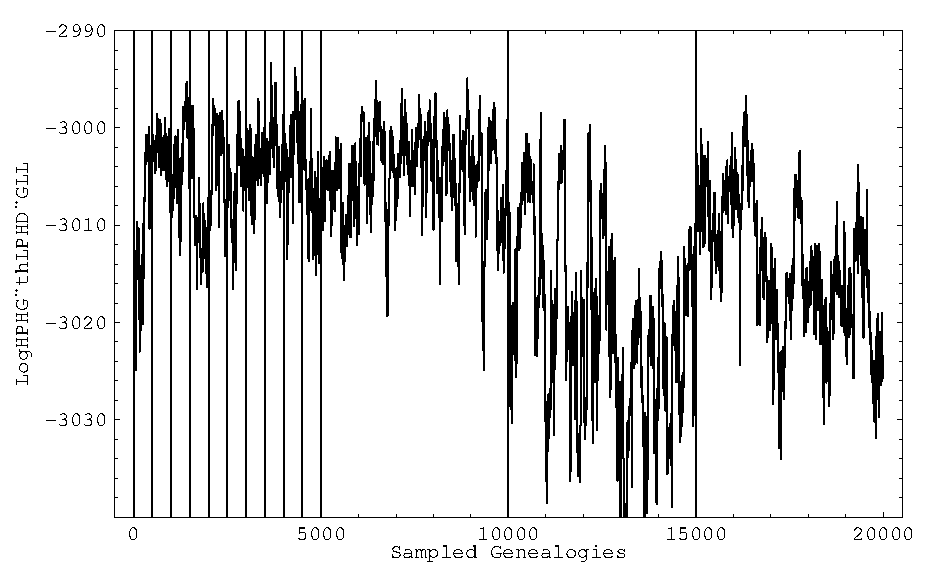
\includegraphics[width=12cm]{mim/mixing}
\end{center}
\vskip -0.5cm
\caption{Data likelihood $\prob(D|G)$ for all sampled genealogies: 
A sample run of migration estimation using 2 populations,
the very long vertical lines mark chain boundaries (10 short and
3 long chains). Totally, $10$ short chains $\times 500$ sampled genealogies 
$+ 3$ long chains $\times$ sampled $5000$ genealogies were sampled out of
total 400,000. The values for not recorded trees are 
not shown.
}
\label{FIGMIX}
\end{figure}
%\end{wrapfigure}

The program is sampling many different genealogies; one can show 
this by plotting
a curve showing on the x-axes all sampled trees and on the y-axis 
the likelihood of the genealogy (in our case this is $\prob(D|G)$
, Figure \ref{FIGMIX}). 
A plot of a sequence of $\prob(\P|G_i)\prob(D|G_i)$ is not 
useful because the genealogies contain different number of time intervals,
and they are {\bf not} comparable. 

One can show that starting from random start parameters, the estimates
converge rather quickly after a few short chains (Figure \ref{fig:convergence}), the updating of
the start parameters over several short chains moves the estimates to the
proper region and the remaining uncertainty is only driven by the
often huge uncertainty about the parameter estimates in the data, 
the likelihood surface is flat for many parameter combinations and 
the data. [checks {\bf (2)}] 
%\begin{wrapfigure}{18}{9cm}
\begin{figure}[hpbt]
%\vskip -1cm 
\begin{center}
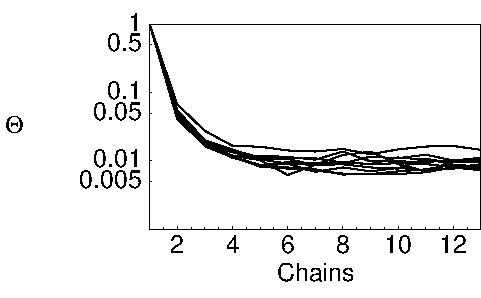
\includegraphics[width=12cm]{mim/convergence_singlepop}
\end{center}
\vskip -0.5cm
\caption{Convergence to the true parameter region. 
Ten runs were started from a $\Theta=1.0$. The data was generated using
a $\Theta=0.01$.
Totally, $10$ short chains $\times 500$ sampled genealogies 
$+ 3$ long chains $\times$ sampled $5000$ genealogies were sampled out of
total 400,000.
}
\label{fig:convergence}
\end{figure}
%\end{wrapfigure}

Comparison with other programs produce similar results. I compared
\migrate with \genetree \citep{Bahlo:2000:IGT} and with
{\tt fluctuate} \citep{Kuhner1998-429}. The comparison with \genetree
used two populations (England and Ghana: 2.5 kb sequence data for the 
beta-globin locus \citep{harding1997-772}) and the results were very similar.
For my paper on n-population I have worked out a 100-locus data set simulation
that shows that \genetree and \migrate deliver the same estimates, and
approximative confidence intervals, although
\genetree is very slow compared to \migrate  for that specific
data set \citep{beerli:2001:mle}.
\vskip 0.7cm 
The comparison with {\tt fluctuate} was for one population, yes you can run \migrate with only one population, and for a data set
created using a $\Theta=0.01$ \migrate delivered $\Theta=0.0123$
with a 50\% confidence interval of $0.08$ to $0.017$, 
while {\tt fluctuate} delivered a point estimate of $\Theta=0.0119$. 
\vskip 0.7cm
In 2007, \citeauthor{roychoudhury:2007:fae} published a new method to infer population-scaled mutation rates, their findings helped me to find a problem with my microsatellite estimator and now accuracy and speed are very similar to their estimator \citep[Figure \ref{fig:msatcomp}][]{beerli:2007:eps}. 
[checks {\bf (1,2)}] 
\vskip 0.7cm
\migrate Version 2.2 and newer print out statistics that help to assess whether the program was run long enough: (1) effective sample size [ESS] and (2) Rubin-Gelman statistic to assess convergence. I am not a strong believer of such measures because they only show the worst problems. For example effective sample sizes of 1000 may seem a lot but it certainly depends on the number of other parameters and the correlation among parameters. The program TRACER (Rambaut et al. 2005) flags effective sample sizes below 100; this is very low for population genetic purposes, I suggest that you strive to get at least 1000 or more for all parameters including the likelihood of the genealogies.
\vskip 1cm
\begin{figure}[hb]

\begin{center}
\includegraphics[width=12cm]{mim/biasfig_revised}

\end{center}
\caption{Mutation-scaled population size estimated from microsatellite data. Bias and absolute error for \migrate version 2.3. Left column: using the stepwise mutation model. Right column: using the Brownian motion approximation, Scale and calculations of bias and absolute error are the same as in Figure 1 in \cite{roychoudhury:2007:fae}. The open squares are the values for $\theta$=32 from their paper.
}
\label{fig:msatcomp}
\end{figure}
\clearpage

\chapter{Quick guide for achieving ``good'' results with {\tt migrate}}
\unitlength=1mm
\begin{picture}(0,0)(0,0)
\put(110,0){
\includegraphics[width=6cm]{mim/read}}
\end{picture}

\section{Monitoring progress}
\subsection{Maximum likelihood inference}
The program will show additional information if the {\bt{progress}} flag is set ({\bt{progress=Yes}} is the default). You can see more with {\bf {progress=verbose}} [I suggest NOT to use this because most of the information is not generaly useful to check convergence, but it is usefule for me to find problems. It uses much more resources and slows the program down].
Below, I show output that uses verbose (to explain some of the output) almost always this is overkill (do not use verbose with parallel runs). 
With {\bt{logfile=filename}} all progress is also directed into this logfile, the default name is 
{\tt logfile}. 
The progress is report similar to the following screen dump fragment
for each chain and each locus. I added a line number which is not part of 
the output (Y means standard progress report, V are the additional lines in verbose mode).
\begin{footnotesize}
\begin{tt}
\begin{verbatim}
01Y 11:49:01   Start conditions: theta={811.90959,0.03487}, M={140.99436,0.00000},
02Y           Start-tree-log(L)=-93.678120
03Y 11:49:01   Equilibrate tree (first 200 trees are not used)
04Y 11:49:03   Long chain   1: lnL=0.21525   ,
05Y            theta={0.04026,0.05527}, M={83.96647,45.78351}
06V            Sampled tree-log(L)={-98.760356 .. -93.035062}, best in group =-93.019453
07V            log(P(g|Param))  -20 to  -18  -16  -14  -12  -10   -8   -6   -4   -2    0   All
08V            Counts                     0    0    0    0    0    0    0    0  144   56   200
09V            Maximization steps needed:   134
10V            Coalescent nodes:  0  1  2  3 
11V              population   0:  *  -  -  - 
12V              population   1:  -  -  -  * 
13Y            Acceptance-ratio = 1095/2000 (0.547500)
.....
14Y 11:49:09   Final parameter estimation over all loci
15Y         
16Y          <paste in correct part>
17Y          
18Y 11:49:09   Program finished
\end{verbatim}
\end{tt}
\end{footnotesize}

The values reported should give some hints how the program progresses 
through the sample space.  The tree likelihoods (line 06V) should go 
steadily up until a peak in the likelihood surface has been reached. 
It can go down through a valley of bad values and either recover on the 
same peak or another one. If this process runs long enough it is 
guaranteed that it will find the global maximum.  But the program is not 
searching the tree-likelihood maximum, it searches through the space 
defined by $\prob(\mathcal D\ |\ \G) \prob(\G\ |\ \P)$ 
and its maximum is not necessarily at the highest tree likelihood. 
The ``histogram" (07V, 08V) of the $ \prob(\G\ |\ \P)$ reflects this. 
The histogram is scaled so that the best value is 0. 
%$$ 
%\frac{\prob(\G\ |\ \P)}{\prob(\G\ |\ \P_0)}.
%$$
If most of the values are in the topmost class the estimate is
probably in good accordance with the trees, otherwise the process
should run longer.  Of course if all genealogies are in the topmost
class one could wonder if the process is sampling different trees at
all, but this can be checked with the acceptance ratio.  If the
Acceptance ratio (13Y) drops below 10\% consider to run the program
with ten time longer chains just to sample enough different
genealogies, so that the parameter estimates are not governed by a few
genealogies only.  
\par 
If the single locus maximization step needs
more than 200 iterations (09V), please send a report, then it should
find most of the time the maximum in fewer than 50 iterations.  
\par
If you have chosen to discard the first few trees using
{\bt{burn-in=value}}, you will see line (3Y).

\subsection{Bayesian inference}
The output for Bayesian inference is more terse, but the same rules apply, except that you should run only one long run because the prior distribution
will deliver many different ``driving" values, convergence issues are still present but less severa as in the ML approach. Under Bayesian inference the effective
sample size and autocorrelation are printed out and give a good idea about how well the run succeeded. The example below is a long parallel run of mutiple microsatellite loci and replication for a total of 180,000,000 updates.
\begin{center}
\includegraphics[width=\textwidth]{mim/ess_auto}
\end{center}
\vskip 1cm
\section{Run time and accuracy}
If you have looked in the menu {\tt Search Strategy} then you saw that
we distinguish between short and long chains. Since the MCMC process
is going from a not so good estimate (the first guess, you specify in
{\tt Start values for Parameters}) to a better estimate along a
``gradient'' on the likelihood surface, the success in recovering the
best parameters is driven by the steepness of this surface. This means
if there is few information in the data, the likelihood surface will
be flat and the estimation process need a long time to wander to a
peak (if at all) . The short chains allow for a burn-in period in
which the the trees and the parameters can equilibrate, for the final
estimate we use only the last of the long chains. The necessary length
of these chains is specified by the number of individuals, length of
sequences and variability of the data. There are no good estimates
what a good length for the final chains should be
\par
For {\it Migrate} it seems that in simulated datasets with around 20
individuals and 10 ``electrophoretic'' loci the truth can be
recovered.
\par
During my simulations for the paper on {\tt Migrate} \citep{Beerli:1999:MLE}, I detected problems 
with the accurate estimation of the migration rate with
start to be obvious with very long sequences (say above 1000bp). 
The first tree is constructed using an UPGMA topology and a Fitch algorithm to 
insert the migrations. This process will insert a minimum of migrations 
onto the tree.
If now the sequences define a good topology for your guessed start 
parameters the program will tend to be stuck with this starting tree.  This is
fine for estimating the population size, but the migrations are not 
well distributed on the tree. 
I recommend that you run longer chains and watch the 
acceptance-rejection, if the program finds about 200 new trees for short chains and about 2000 trees for long chains or more  then the estimation process should be fine.
If in your initial run you see acceptance ratios of only around 2\% you should 
definitely increase the length of the chains, or use the option {\bt{ moving-steps}}. 
When after some runs
you see that the program returns hugely different values, for example
the profile likelihood curves exclude the parameter estimates of other
runs, you should also consider running multiple chains 
at different temperatures or use replication (see {\bf Search Strategy}).
Most likely, there are
sets of genealogies that are not that well connected and with short
chains the program will settle in one solution. 
Currently there is no way to check
which of the independent runs fits the data better because the 
reported likelihoods are relative and not absolute and this makes 
it impossible to compare different runs. 

\section{Quick guide for achieving ``good'' results with {\tt migrate}}
Of course this is not a fool proof guide, then it's easy to give advice with 
data simulated using the same sequence model as the inference program.
\par
{\bf FIRST: make sure that your data is correct}. Miscounts of individuals,
sequence length, number of loci etc can produce funny errors.
\begin{itemize}
\item Set parameters in the {\bf Search Options} to very low values, 
e.g to something
below 100 for sampling increment and the chains to something like 2, also
Turn off the profile and plot option, but set {\tt print the data}
 in the {\bf Input/Output} menu.
\item run the program an check if the number of individuals read is correct,
and if all the data was read, and if the program produces numbers 
in the output. If the program crashes before the menu there is an error 
in the {\tt parmfile}, if it crashes shortly after the menu most likely 
there is some error in
the infile. If it crashes at the end, most likely there is a programmer's 
bug :-(.
\item Once it is clear that the program is able to run, use the default options
to start a first run. If you have written a {\tt parmfile} you should rename 
or destroy it.
\end{itemize}

Monitor the progress by looking at the intermediate parameter estimates:
\begin{itemize}
\item Check the log on the screen or the logfile, if the data-likelihood of 
the start tree for each chain is always improving then consider to lengthen 
the increment between the sampled genealogies (e.g. {\tt short-inc=100}) or
supply 
your own distance matrix ({\tt distfile} option), or give own starting 
values or run more short chains (e.g. {\tt short-chain=20}).
\item Gelman's convergence criterium: My implementation of this criteria
is not completely correct, then \migrate\ is using two consecutive chains
to calculate the criterium, whereas Gelman used chains with ``overdispersed'' 
starting points. If the values are close to 1 (Gelman uses $R < 1.2$) then 
we can assume that the chains are sampling from the stationary distribution 
and that our parameter estimates are OK, but of course, this is no guarantee
for success then when the sampler is sampling only around one probability mountain and
does not know that another much higher mountain exist, the results will be wrong.
\end{itemize}  
But, besides monitoring progress, I would:
\begin{itemize}
\item Run {\it Migrate} with the default values using ${\rm F_{ST}}$ to find
the start parameters.
\item Rerun, using the obtained parameter estimates of the last run. Be careful not to take this advice too literally: start parameters of zero (0.0) are very bad starting points for parameters where you expect nozero values, if the preliminary run suggests a parameters is zero, use some arbitrary value: for example for $\Theta$ and DNA data I would use 0.005 
\item If the results do not change much , perhaps you can stop. Otherwise
increase the length of the chains, increasing the increment 
({e.g. \bf short-inc=100} and {\bf long-inc} does not
increase memory usage, but run-time. 
You can also increase the number of sampled
genealogies ({\bf short-sample} or {\bf long-sample}).
E. g. increase it by a factor of 10.
\item Change the random number seed and check if you get similar results.
\item Use the heating scheme if you get wildly different results and
have low acceptance ratios.
\item Run with {\tt replicates=YES:10} and perhaps also using
{\tt randomtree=YES}, but beware this will run 10x longer then your single
run.
\item Microsatellite and Electrophoretic data should experiment with
lowering the number of sampled genealogies (if they have many loci), because
otherwise the runs will take forever, try to run migrate on a parallel machine 
(based on MPI) that would distribute the loci
onto different machines, read the chapter "Parallel migrate".
\end{itemize}


% !TEX root = migratedoc.tex
\chapter{Presentation of results}

\section{Maximum likelihood inference}
There are several differences between the \ma and \ba output. The outfput exists typically in two files
a textfile called outfile (default name) and a PDF called outfile.pdf, for changing these names consult the 
input/output menu. The maximum likelihood analsysi writes to a PDF file but because of time constraints
I never completely finished that transition (perhaps next year), therefore for \ma use the textfile as the main
output, EXCEPT if you are interested in the distribution of the migration and coalescence events through time,
that is only plotted into the PDF (see below).

Contents of the output in \texttt{ outfile}: Some of the output options vary
according to the datatype.  + = always present, o = optional, Default = $\star$
\newcommand{\st}{$\star$}
\smallskip
\begin{center}
\begin{tabular}{l p{10cm} c}
\hline
Item & Description  & Status\\
\hline
List of options & {all used options are specified} & +\\
Summary of data & {(Too) short data summary} & +\\
Dataset & Print of the dataset & o\\
MCMC estimates & {List of the estimated parameters for each locus and the mean} & +\\
Shape $\alpha$ & {Estimation of the shape parameters $\alpha$ for the variation of the mutation rate}  & o\\
\fst table & {Table of the possible start values generated with a \fst estimator}  & o \\
plots & {plot of the likelihood surface in outfile} & o\st \\
  & {plot of the likelihood surface into mathfile} & o\\
$\alpha$-histogram & {Table of shape values versus log(likelihood), $\alpha$ is varying whereas the other parameters are held constant at the maximum of the surface.} & o\\
Profiles & {Profile likelihood tables} & o\st \\
Percentiles & {Percentiles table, summary of profile tables} & o\st\\
Event histograms & {Distribution of events over time} & o\\
\hline 
\end{tabular}
\end{center}
The $F_{ST}$ calculations are based on mean differences in populations compared
to mean differences between populations, for more information you should consult \cite{maynardsmith:1970:psp, nei:1972:igd, beerli:1999:mle}, .

\subsection{Walk through an outfile}
The following output pieces are from \texttt{ outfile.seq} in the \texttt{ example} directory.
\subsubsection{Title and Options}
\begin{center}
\begin{boxedminipage}{6in}
\begin{footnotesize}
\ttfamily{
\begin{verbatim}
 =============================================
   An example with sequence data
 =============================================
  MIGRATION RATE AND POPULATION SIZE ESTIMATION
  using Markov Chain Monte Carlo simulation
  =============================================
  Version 2.0.3

  Program started at Sat Dec 18 19:56:23 2004
         finished at Sun Dec 19 01:22:31 2004
     
Options in use:
---------------
Datatype: DNA sequence data
Random number seed (with internal timer)           1103417783
Start parameters:
   Theta values were generated  from the FST-calculation
   M values were generated from the FST-calculation
Migration model:
   Migration matrix model with variable Theta  
Mutation rate is constant for all loci
Analysis strategy is                          Maximum likelihood
Markov chain settings:
   Short chains (short-chains):                           10
      Trees sampled (short-inc*samples):               20000
      Trees recorded (short-sample):                    1000
   Long chains (long-chains):                              3
      Trees sampled (long-inc*samples):               200000
      Trees recorded (long-sample):                    10000
   Averaging over replicates:                              2
   Static heating scheme
      4 chains with  temperatures
       1.00, 1.57, 2.71, 5.00
      Swapping interval is 1
   Number of discard trees per chain:                  10000
Print options:
   Data file:                               infile.check-mig
   Output file:                                      outfile
   Print data:                                            No
   Print genealogies:                                     No
   Plot data: Yes, to outfile and mathfile                  
              Parameter: {Theta, M}, Scale: Log10, Intervals: 36
              Ranges: X-    M: 0.000100 - 100.000000
              Ranges: Y-Theta: 0.000100 - 100.000000
   Profile likelihood: Yes, tables and summary             
             Percentile method
             with df=1 and for Theta and M=m/mu
\end{verbatim}
}
\end{footnotesize}
\end{boxedminipage}
\end{center}
This is the title and options part. Don't cut away the options, so you will 
still
know a few weeks later with what kind of options and how long you
run the program.
\newpage
\subsubsection{Summary of the data}
\begin{center}
\begin{boxedminipage}{6in}
\begin{small}
\ttfamily{
\begin{verbatim}
Summary of data:
---------------
Datatype:                                       Sequence data
Number of loci:                                             2

Population                                    Locus  Gene copies
----------------------------------------------------------------
  1 Tallahassee                                  1     20
                                                 2     20
  2 Sopchoppy                                    1     20
                                                 2     20
  3 St._George Island                            1     20
                                                 2     20
Total of all populations                         1     60
                                                 2     60


Empirical Base Frequencies
------------------------------------------------------------
Locus     Nucleotide                        Transition/
          ------------------------------  Transversion ratio
          A       C       G       T(U)
------------------------------------------------------------
   1      0.2515  0.2730  0.2283  0.2472       2.00000
   2      0.2465  0.2350  0.2627  0.2557       2.00000

\end{verbatim}
}
\end{small}
\end{boxedminipage}
\end{center}
The data summary is (too) short, and self explanatory, you can also print
the data (not shown). Print the data the first time you use the program with
your data and check if it was read correctly: I control the first and the last
individual in a population and check a few sites at both ends of the sequence.
If the program crashes shortly after the start, almost certainly the data
contains some trouble. The most common error is having the wrong number
of individuals and/or number of sites, or having miscounted the number of characters in the individual name.
\newpage
\subsubsection{Parameter estimates}
\begin{center}
\begin{boxedminipage}{6in}
\begin{small}
\ttfamily{
\begin{verbatim}
==============================================================================
MCMC estimates 
==============================================================================
Population [x] Loc.  Ln(L)   Theta    M [m/mu] [+=receiving population]  
                             [xNe mu]    1,+     2,+     3,+    
-------------- ---- -------- -------- ----------------------------------------
 1: Tallahasse  1 1   11.406  0.04326 ------- 22.9291  0.0000 
                1 2    0.875  0.04006 -------  0.0000  0.0000 
                1 A    1.754  0.04009 -------  0.0000  0.0000 
                2 1    2.463  0.03418 -------  0.0000 11.8760 
                2 2    3.246  0.04276 -------  4.1693 12.4264 
                2 A    4.158  0.04214 -------  3.8056 12.1477 
                All   20.696  0.04330 -------  8.6572  0.0000 
 2: Sopchoppy   1 1   11.406  0.01553  5.6584 -------  3.2363 
                1 2    0.875  0.01996 12.0396 -------  0.0000 
                1 A    1.754  0.01993 12.0679 -------  0.0000 
                2 1    2.463  0.00918  0.0000 ------- 14.9951 
                2 2    3.246  0.01485  0.0000 ------- 16.6994 
                2 A    4.158  0.01444  0.0000 ------- 16.5949 
                All   20.696  0.01283  0.0000 -------  2.0536 
 3: St._George  1 1   11.406  0.00969  0.0000  0.0000 -------
                1 2    0.875  0.01125  0.0000  5.8414 -------
                1 A    1.754  0.01124  0.0000  5.8325 -------
                2 1    2.463  0.01174 13.0240  0.0000 -------
                2 2    3.246  0.01025 20.5578  0.0000 -------
                2 A    4.158  0.01039 19.7503  0.0000 -------
                All   20.696  0.01088  3.4871  3.2021 -------

Comments:
 The x is 1, 2, or 4 for mtDNA, haploid, or diploid data, respectively
There were 10 short chains (1000 used trees out of sampled 20000)
  and 3 long chains (10000 used trees out of sampled 200000)
  Static heating with 4 chains was active
  COMBINATION OF 2 MULTIPLE RUNS)
\end{verbatim}
}
\end{small}
\end{boxedminipage}
\end{center}
This is the main output of the program. For each population there is a list
of all estimates for each locus and each replicate and their over-all-replicate and over-all-loci estimates. The replicate summary estimates are not simple averages but use a method devised by Geyer (1994: reverse logistic regression). The summary over loci is summing up the likelihood curves under the assumption that each locus is independent of the other (a rather save assumption as long one is not working with multiple mtDNA or Y-chromosome loci).
%\par
%The ln(L) is the maximum log likelihood.
%This value is a ratio $ln(L) = ln(L(\P)/L(\P_0))$ and is always above 0.0 in this table. The parameter $\P_0$ are
%different between different runs of the program and therefore you cannot
%simply compare between different runs.
%\par
%The column marked Theta ($\Theta$) gives the population sizes for 
%each population and each locus, of course the number of individuals
%in that population $N_e$ is for all loci the same, and the variance you see
%is (a)  the variance of the sampler, 
%(b) stochastic variance due to the coalescence
%process, (c) variance of the mutation rate.
%The migration parameter $\M$  table is to read the following way:
%in population 1, the \textbf{ 2,+} means that the immigration from population two into one is $\M_{21}=8.6572$.
%in population 2 the \textbf{ 1,+} means that the immigration from population one into two is $\M{12}=0.0000$
%If the program is also allowing for variable mutation rate (you don't want to
%use that with only few loci), then you will get also an estimate for the 
%shape parameter alpha ($\alpha$) for the distribution of the mutation rates.  
%
%\subsubsection{\fst table}
%This will be shown when print-fst=YES is set. If you want to use this you need to reread the appendix of Beerli and Felsenstein (1999). It is merely used as a starting 
%value for the Maximum likelihood estimates. The table are similar to the table
%of the MCMC estimates.

%\subsubsection{Likelihood surface plots}
%For each population and each locus there will be a summary contour plot
%for all immigrations and all 'emmigrations'. These plots give some information
%about the confidence you should have in the estimates. Keep in mind that
%even with two populations there are 4 parameters and the likelihood.
%A plot is a kind of diagonal through this high dimensional space (in this
%example: 10 dimensions). The contour plots in the \textbf{outfile} are very crude, but the contour data is also written into the \textbf{mathfile} and this can be displayed with programs such as mathematica (see example program earlier) or gnuplot and could look like the following contourplot, it is the same as the left graph shown on the next page. The graph shows the total immigration rates, expressed as $\M$ versus the population size $\Theta$.
%\begin{center}
%\begin{boxedminipage}{4in}
%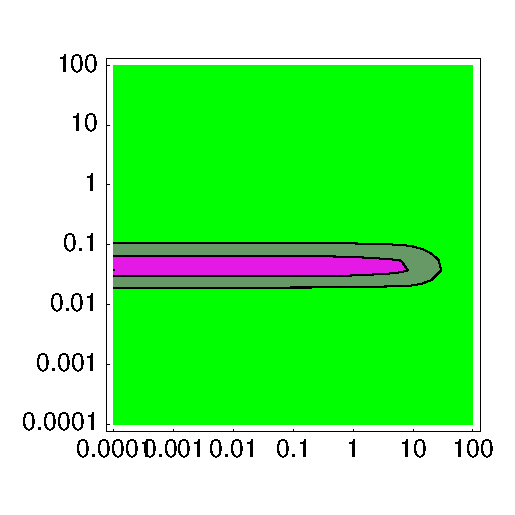
\includegraphics{mim/mathfilegraph}
%\end{boxedminipage}
%\end{center}
%\newpage
%\begin{center}
%\begin{boxedminipage}{6.5in}
%\begin{small}
%\ttfamily{
%\begin{verbatim}
%[the figure is edited so that it fits better on the page]
%n-Likelihood surfaces for each of the   3 populations
%-------------------------------------------------------
%
%Legend:
%   X = Maximum likelihood
%   * = in approximative 50% confidence limit
%   + = in approximative 95% confidence limit
%   - = in approximative 99% confidence limit
%X-tickmarks are (1) 0.000100, (2) 0.001585, (3) 0.025119
%                (4) 0.398107, (5) 6.309573, (6) 100.000000
%Y-tickmarks are (1) 0.000100, (2) 0.001585, (3) 0.025119
%                (4) 0.398107, (5) 6.309573, (6) 100.000000
%
%Over all loci
%
%    x-axis=   M [xNm = effective population size * migration rate = Theta * M
%                  M   = migration rate / mutation rate = m/mu],
%x=1, 2, or 4 for mtDNA, haploid, or diploid data
%    y-axis = Theta,
%    units = see above
%Population 1: population__number___0
%  **Average** immigration: M=0.000100, Theta=0.037276, log likelihood=20.332327
%  **Average** emigration: M=1.930698, Theta=0.037276, log likelihood=20.769244
%[Remember: the maximum values are from a grid]
%
%          Mean(Immigration)                       Mean(Emigration)
%
%      1      2      3      4      5      6      1      2      3      4      5      6
%     ++------+------+------+------+------++    ++------+------+------+------+------++
%   6 +                                    +    +                                    +
%     |                                    |    |                                    |
%     |                                    |    |                                    |
%   5 +                                    +    +                                    +
%     |                                    |    |                                    |
%     |                                    |    |                                    |
%   4 +                                    +    +                                    +
%     |                                    |    |                                    |
%     |                                    |    |                                    |
%     |                                    |    |                                    |
%     |++++++++++++++++++++++++++++++-     |    |+++++++++++++++++++++++++++++++--   |
%     |******************************++    |    |********************************++  |
%     |X******************************+-   |    |*************************X*******+- |
%   3 ++++++++++++++++++++++++++++++++-    +    ++++++++++++++++++++++++++++++++++-  +
%     |                                    |    |                                    |
%     |                                    |    |                                    |
%     |                                    |    |                                    |
%     |                                    |    |                                    |
%   2 +                                    +    +                                    +
%     |                                    |    |                                    |
%     |                                    |    |                                    |
%   1 +                                    +    +                                    +
%     ++------+------+------+------+------++    ++------+------+------+------+------++   
%      1      2      3      4      5      6      1      2      3      4      5      6
%
%\end{verbatim}
%}
%\end{small}
%\end{boxedminipage}
%\end{center}
%\subsubsection{Likelihood ratio tests}
%The likelihood ratio test printout consists of a legend that explains the likelihood ratio tables and the tables themselves. the lefts side states the hyopthesis and the right side shows the associated values.
%\begin{center}
%\begin{boxedminipage}{6in}
%\begin{small}
%\ttfamily{
%\begin{verbatim}
%==============================================================================
%Likelihood ratio tests
%==============================================================================
%Over all loci
%Legend for the LRT tables
%-------------------------------------------------------------------------------
%Null-Hypothesis: your test model         | Log(likelihood) of test model
%=same=                                   | Log(likelihood) of full model
%full model (the model under which the    | Likelihood ratio test value
%genealogies were sampled)                | Degrees of freedom of test
%[Theta values are on the diagonal of the | Probability*
%Migration matrix, migration rates are    | Probability**
%specified as M]                          | Akaike's Information Criterion***
%                                         | Number of parameters used
%-------------------------------------------------------------------------------
%  *) Probability under the assumption that parameters have range -Inf to Inf
% **) Probability under the assumption that parameters have range 0 to Inf
%***) AIC: the smaller the value the better the model
%          [the full model has AIC=1125.401453, num(param)=9]
%-------------------------------------------------------------------------------
%H0: 0.0458 5.8386 5.3308 5.8386 0.0169 2.1822 5.33 | LnL(test) = -1606.113074
%    2.1822 0.0103                                  | LNL(full) = -553.700726
% =  0.0458 9.4132 0.0000 2.2639 0.0169 4.3644 10.6 | LRT       = 2104.824696
%    0.0000 0.0103                                  | df        = 6
%[ *, s, s, s, *, s, s, s, *,]                      | Prob      = 0.000000
%                                                   | Probc     = 0.000000
%                                                   | AIC       = 3226.226148
%                                                   | num(param)= 7
%-------------------------------------------------------------------------------
%\end{verbatim}
%}
%\end{small}
%\end{boxedminipage}
%\end{center}
%\newpage
%\subsubsection{Profile likelihoods}
%\begin{center}
%\begin{boxedminipage}{6in}
%\begin{small}
%\ttfamily{
%\begin{verbatim}
%Profile likelihood for parameter Theta_1
%Parameters are evaluated at percentiles.
%-------------------------------------------------------------------------------
%Per.  Ln(L)     Theta_1     *Theta_1*   Theta_2     M_21       M_12      
%-------------------------------------------------------------------------------
%0.01  -3.645      0.0223     0.0223     0.0297    81.9303   293.8230 
%0.05  -2.065      0.0240     0.0240     0.0297    81.9441   294.2779 
%0.10  -1.329      0.0250     0.0250     0.0297    81.9766   294.5011 
%0.25  -0.284      0.0266     0.0266     0.0296    82.0709   294.7953 
%0.50   2.878*     0.0457     0.0457     0.0286    88.4385   273.2104 
%0.75   0.324      0.0789     0.0789     0.0279    96.2738   252.5011 
%0.90  -1.065      0.0900     0.0900     0.0277    97.4555   251.1683 
%0.95  -1.910      0.0966     0.0966     0.0277    98.0544   250.5631 
%0.99  -3.884      0.1119     0.1119     0.0276    99.2213   249.4557 
%-------------------------------------------------------------------------------
%\end{verbatim}
%}
%\end{small}
%\end{boxedminipage}
%\end{center}
%
%The profile likelihood table show how the parameters vary
%when we hold one parameter constant. In the default setting the program tries to
%find the parameter values that are at the percentiles.
%How is this done for $\Theta_1$:
% calculate the likelihood value for
%\begin{enumerate}
%  \item a few values smaller and bigger than the ML-estimate. 
%  \item calculate a spline
%function. 
%\item find the $\Theta_1$ that is at the percentile $x$ using the
%splines. 
%\item recalculate the likelihood and maximize the other parameter again
%using the full formula.
%\end{enumerate} 
% In the example, $\Theta_1$ varies almost independently from the others, but looking more closely it seems that $\Theta_2$ slightly
%shrinks while $\Theta_1$ grows.
%
%Sometimes, the algorithm to find the percentiles fails, in this case  the program prints instead of the precentile values \texttt{***} and warns that it failed to calculate the percentiles. The calculates likelihoods and parameter values are still correct but simply not at the percentile values. Earlier versions of the program did not tell the user about this shortcoming.
%\newpage
%\subsubsection{Summary of profile likelihood tables}
%\begin{center}
%\begin{boxedminipage}{6in}
%\begin{small}
%\ttfamily{
%\begin{verbatim}
%===============================================================================
%Summary of profile likelihood percentiles of all parameters
%===============================================================================
%
%Parameter                          Lower percentiles
%            -------------------------------------------------------------------
%                0.01          0.05          0.10          0.25          0.50
%-------------------------------------------------------------------------------
%Theta_1         0.02228       0.02399       0.02497       0.02664       0.04567
%Theta_2         0.00946       0.01188       0.01331       0.01567       0.02857
% M_21          30.53718      36.49126      39.97529      46.64759      88.43845
% M_12         114.08445     132.49441     143.22648     163.32323     273.21045
%
%
%Parameter                          Upper percentiles
%            -------------------------------------------------------------------
%                0.50          0.75          0.90          0.95          0.99
%-------------------------------------------------------------------------------
%Theta_1         0.04567       0.07889       0.09003       0.09660       0.11190
%Theta_2         0.02857       0.05709       0.07586       0.09833       0.15052
% M_21          88.43845     201.06595     215.26333     225.18048     245.85767
% M_12         273.21045     805.85153     896.08361     957.07762    1083.66503
%-------------------------------------------------------------------------------
%\end{verbatim}
%}
%\end{small}
%\end{boxedminipage}
%\end{center}
%
%This summarizes only the likelihood and profile parameter column from the
%profile likelihood tables and can be used to give some idea about the 
%confidence you should have into the estimates.
%$\Theta_1$ has a \textbf{approximative} 90\%-confidence interval from 0.02399 to 0.09660
%with a best estimate of 0.04567.
%(the data was simulated with a $\Theta_1=0.05$.
%If the percentile calculation failed, this summary plot needs to be evaluated carefully, the program warns about possible problems by printing an \texttt{*} next to then value in question.
%\newpage

\section{Bayesian inference}

\subsection{Walk through an outfile}

The main output of a Bayesian run contains of the following table that summarizes the posterior distribution and an acceptance ratio table. The table of the posterior distribution is characterized for each locus and each parameter and percentiles, median, mode, and mean. The posterior distribution over all loci is also presented graphically (Figure \ref{BAYESTABLEHIST}). 

\begin{figure}[htb]
\begin{center}
\includegraphics[scale=0.6]{mim/bayestable}\\
\includegraphics[scale=0.6]{mim/bayeshist}
\end{center}
\caption{Table and Figure example of a Bayesian posterior distribution. \label{BAYESTABLEHIST}}
\end{figure}


%The acceptance ratio tables give some idea whether the Markov chains has mixed and explored many different values.
%\begin{center}
%\begin{boxedminipage}{6in}
%\begin{small}
%\ttfamily{
%\begin{verbatim}
%Bayesian estimates
%==================

%Locus Parameter  2.5%      25.0%   median    75.0%   97.5%     mode     mean
%-----------------------------------------------------------------------------
%    1  Theta_1   0.00986  0.00434  0.00932  0.00000  0.07356  0.00602  0.01272
%    1  Theta_2   0.00439  0.00171  0.00372  0.00000  0.06915  0.00274  0.00448
%    1  M_2->1        644   614.46   623.20     0.00  3654.57   189.32   872.45
%    1  M_1->2        197   197.11   193.09     0.00  6890.91     4.02   369.93

%

%Acceptance ratios for all parameters and the genealogies (Locus 1
%---------------------------------------------------------------------

%Parameter           Accepted changes            Ratio
%Theta_1                 90646/125195            0.72404
%Theta_2                 61965/125195            0.49495
%M_2->1                  80238/125194            0.64091
%M_1->2                  63487/125194            0.50711
%Genealogies             22270/500000            0.04454
%\end{verbatim}
%}
%\end{small}
%\end{boxedminipage}
%\end{center}
% plot of a credibility set etc
\newpage
\section{Histograms over time}
\subsection{Events through time}
\migrate allows to investigate the pattern of events through time, the histograms represent the frequency of recorded events during the MCMC run, the location of these events in time are determined by the data (that is what we want to see) but depends on the length of runs, and how well the genealogies were explored (that is what we want to have no influence!). \migrate is assuming the all the events in every time units come from the same prior distribution (BA) or driving value (MA). For simulated data from populations that are constant in size through time and that exchange migrants at a constant rate, we expect distributions that look similar exponential decay. If either the data was generated by a process that is not constant through time the histogram will look different (figure \ref{MIGPROBHIST}). The time is measure in unites of generation / mutation rate per generation (and site) .
\begin{figure}[htb]
\begin{center}
\includegraphics[scale=0.8]{mim/frequencyM}
\end{center}
\caption{Frequency of migration events between between two populations through time. Today is left on the graph; units are generation per mutation rate 
\label{MIGPROB}}
\end{figure}
\migrate also prints out tables that report average time for migration and coalescence events for all events and for the most recent common ancestors, and that supplies the probability in which population the sample originated (Figure \ref{MIGPROBTABLE}). This seem to work fine with equal sample sizes , but may be skewed with unequal sample size (for example for two populations: 100 and 10). Unequal sizes may need much longer run time to say some thin with confidence. In addition, a single locus may not give really relevant results, use multiple loci if you can.
\begin{figure}[htb]
\begin{center}
\includegraphics[width=8cm]{mim/sumfreq}
\includegraphics[width=8cm]{mim/timeMRCA}
\end{center}
\caption{Left: Tables of frequencies and average time for all events. Right: Table of the probability of the location of the most recent common ancestor. \label{MIGPROB}}
\end{figure}

\subsection{Skyline plots}

\begin{figure}[!h]
\begin{center}
\includegraphics[scale=0.9]{mim/skylineTheta}\\

\includegraphics[scale=0.9]{mim/skylineM}
\end{center}
\vskip -1cm 
\caption{Skyline plot of a population that recently increased strongly , the time is in units of mutation-scaled generations. Top: population size, bottom: one example immigration rate into the population shown on top.
\label{SKYPLOT}}
\end{figure}

\migrate has its own version of skyline plots \cite{strimmer:2001:edh,Shapiro:2004:RFB,Drummond:2005:bci}. \migrate reports averages and standard deviation of expected parameter values calculated from the genealogy. The proposal for all timeintervals uses the constant population size and migration rate, so it is different from  \cite{Drummond:2005:bci} and certainly needs more evaluations. \migrate can summarize over multiple loci, take into account several data types, and reports the parameters changes through time also for migration parameters. \migrate has several short-comings: for example it assumes that the mutation rate is constant per locus, which make affect results for some data sets, but because \migrate is typically used for populations within species or very closely related species, I hope that the mutation rate of a specific locus will not change considerably.

A legend for these plots is printed toward the end:
\begin{footnotesize}
\begin{verbatim}
Skyline plots: 
Skyline plots visualize the changes of population sizes and migration rates through time 
(today is on the left side and time is measured into the past. The time scale is in units of 
expected mutations per generation. To calculate the absolute time scale you must supply an 
mutation rate per year and the duration of a  generation in years in the data option. 
You can calculate the absolute time by multiplying the scale by generation time times 
mutation rate per year (per site for DNA; per locus for all other datatypes). 
With estimated mutation rate only the combined rate modifier is plotted. 
[this will change to  mutation rate plot]. 
The gray bars cover one approximate standard deviation up and down from the expected value. 
The bar with different shades of gray on top of each plot indicates the number of values that were used 
to calculate the expected value, white means there are very few and black means. 
that there were man thousands of samples per bin. 
On some plots one can see red squares below the grayscale bar, these suggest that either the 
upper quantile and/or the main value was higher than the visible part of the  axis. 
Event histograms: 
All accepted events (migration events, coalescent events) are recorded and their frequency 
are shown as histograms over time with recent time on the left side. The frequency plots of 
populations with constant size and constant immigration rates show histograms that are similar 
to exponential distribution, if the populations come from a divergence model without migration 
then the frequency of migration events can show a peak in the past.
\end{verbatim}
\end{footnotesize}
\chapter{Output that is not part of the outfile}
\migrate writes the raw data that is used to generate the histograms and tables in the PDF and the textfile into several files, such as the \textsl{bayesfile}, \textsl{bayesallfile}, \textsl{mighistfile} and the \textsl{skylinefile}. Each file contains a header that gives you some idea what the values mean and you can process these files by yourself using graphing programs (or \tracer). I highlight here a use of the the print-tree option.
 
\section{Potential genealogy plots}
\migrate allows to record the best genealogy visited in the course of the MCMC run, this treefile contains migration events and currently only the program \texttt{ eventtree} (ET) (Palczewski and Beerli unpubl. -- popgen.scs.fsu/et ) can plot these events. Remember this is not necessarily the best possible tree for the data, but the most likely visited tree, in tests with small dataset we could show that with real species tree \migrate recovers the topology, but because it does not optimize branch length, will make errors on the length of the branches, it also assumes a clock.
\begin{figure}[bh]
\centering \includegraphics[width=10cm]{mim/human_tree}
\caption{Best visited genealogy of a 3 population run with Neanderthals, modern humans, and chimpanzees. The arrows on the tree mark migration events --  there is very little power to pinpoint these migration events and the events shown are a haphazard sample of many possible migration events that happen to occur on the topology that is most compatible with the data, The color was added using Adobe Illustrator.\label{MIGTREE}}
\end{figure}

\newpage
\chapter{Diagnostics}
\migrate prints out several diagnostics, these diagnostics are not sufficient to judge whether your data was run successfully, but you should run the program minimally two times to compare the results and not trust the diagnostics. The acceptance/rejection ratios for all parameters (BA) and the genealogy (MA, BA) give some idea about how many new parameters or trees are in the MCMC sample, if the ration is very low the autocorrelation will be high and the effective sample size of trees and parameters will be low. For MA a statistic described by Gelman and Rubin \cite{kass:1998:mcm} can be used to get some idea about convergence. The Gelman-Rubin statistic is broken for some of the analysis option, but I believe that multiple runs from different start settings (different start parameter and random tree) are a great way to explore the behavior of the MCMC run(s).

The last page of the output can contain  \textbf{ Warnings} that suggest whether some parameters did not converge or not (Figure \ref{ESS}). 
\begin{figure}[bh]
\begin{center}
\includegraphics[width=8cm]{mim/acceptance}
\includegraphics[width=8cm]{mim/ess}
\includegraphics[width=8cm]{mim/warnings}
\end{center}
\caption{Acceptance Ratios, Effective sample size and autocorrelation, and Warnings of a run.
\label{ESS}}
\end{figure}

\newpage

% !TEX root = migratedoc.tex
\chapter{Installation}
\subsection{Binaries}
On UNIX system unpack with \texttt{ tar xvfz migrate.[system].tar.gz} or\\ \texttt{ gunzip -c migrate\VERSION .[system].tar.gz | tar xf -}.
This builds a directory \texttt{ migrate-\VERSION}
with a subdirectory \texttt{ examples},
the files \texttt{ README, HISTORY}, and the programs 
\texttt{ migrate} and \texttt{ migrate-n}. 
The program can be moved to a location like \texttt{ /usr/local/bin} 
and the documentation (HTML files are in documentation/migratedoc) to
your HTML directory (e.g. \texttt{ /usr/local/etc/httpd/htdocs}).
On Powermacs or Windows machines double click the archive 
and a folder system similar the UNIX directories above will be created.

\subsection{Source}
The program is known to compile on
every UNIX machine that has a decent ANSI compatible compiler.
And on the following non-UNIX machines:  INTEL (Windows 2000, xt, vista?).

\subsubsection{UNIX (Linux, BSD Unix, MacOSX)}
\begin{enumerate}
\item {\bt{gunzip -c migrate\VERSION .tar.gz $|$ tar xf -} or\\
\bt{tar xfz migrate\VERSION .tar.gz}}
   this creates a directory "migrate-\VERSION " with "src", ``contribution'',  and "examples" in it.
\item \texttt{ cd migrate-\VERSION }
\item \texttt{ ./configure} \\(this scripts checks your system and will report 
functions the program needs, if a function is not, it will report an error,
which I need to know. I assume that your machine has \texttt{ gcc} installed,
but \texttt{ configure} tries to be smart about other compilers: 
on SGI and DEC ALPHA without \texttt{ gcc} it will use the native 
$cc$ compiler with the approriate options. You can force this behavior
with bash shell: CC=cc ./configure, in csh shell: env CC=cc ./configure

\item  \texttt{ make}  \\
 (please report warnings and especially errors)
 This produces an optimized binary for your computer, if your computer has multiple CPUs or core, you can try to compile
 using \texttt{ make thread}, this produces a binary that can use multiple processors for heated runs, this is good but parallel
 runs on such computers use more CPU cycles.
 
 The result should be a binary \texttt{ migrate} in the migrate directory.
If you have a multiprocessor machine that has the POSIX thread library
installed (the configure script searches for libpthread and pthread.h)
try to use \texttt{ make thread}, this will allow to run the heated chains
in parallel and so should speed up the program if you use heating.
\item \texttt{ make install} \\ (this will install the program and man-page into usr/local/bin, /usr/local/man/man1
   ; you need to be root to do this; this step is not necessary)
\end{enumerate}


\chapter{Parallel \migrate}
This text describes how you can improve the performance of \migrate\ 
when you have more than one locus and more than one computer at 
your fingertips. You can parallelize migrate runs 
(1) using a virtual parallel architecture with a message-passing 
interface (MPI) or (2) by hand.
The hand-version works but is cumbersome, 
the MPI-version runs fine on clusters of MacOSX workstations, dedicated clusters of Linux machines, 
AIX parallel machines (Regatta; SP3, SP4).

\section{I. Using the standard Message passing interface (MPI)}

\begin{enumerate}
\item  Secure as many computers for the analysis as you have loci or parameters
    in your dataset. Make sure that all computers can talk to each
    other. Currently my program will only work if they are a flavor of 
    UNIX (e.g. LINUX or MACOSX). Of course, you need an account on all 
    the machines.
  \begin{itemize}
  \item   Download OpenMPI from  http://www.openmpi.org [I use version 1.2.5] (Macintosh computers with the Leopard operating system -- MacOS 10.5 have this already built-in, use \texttt{ fastmigrate-n})
    \item install on all machines (if this is to complicated for you ask a
      sysadmin or other guru to help:\\
      ~~~~~~\texttt{ ./configure }
      There are several options that may or may not be helpful in your environment
     \item prepare a file ``hostsfile" according to the specs in the openmpi distribution, the master node
      needs to be the first machine mentioned.
      my ``hostsfile" looks like this:\\
      \ttfamily{
      ciguri node=2\\
      zork  node=1\\
      nagual node=32
      }	      
\item make sure that you can access all machines [using ssh]
     without the need to specify a password, see man ssh-keygen and man ssh
     if you have firewalls installed on your individual systems then you would need to allow
     the individual machines to open/request "random" ports on the other machines. 
     On MacOSX machines this is a common problem because the machines may run local firewalls.
\item change into the migrate-2.4/src/ directory
      configure and then use "make mpis-pretty" 
\end{itemize}      

\item If your machines have no cross-mounted file system,
    you need to make sure that the program is all
    in the same path e.g. /home/beerli/migrate-test/migrate-n and on EVERY machine.
    
    
\item Compile migrate, you need to follow the instructions in README. Essentially you need to do\\
\texttt{
     ./configure\\
     make mpis
     }
     
     The configure command sets up the Makefile etc. 
     \texttt{make mpis-pretty} compiles for parallel machines.
     
\item Try run the following command from the src/example directory
\begin{itemize}
  \item    \texttt{mpirun  -np 7 --host hostfile ../migrate-n parmfile.testbayes -nomenu}
    [ 6 loci will be analyzed at at the same time,
     the log is not very comprehensive because all 7 processes
     write to the same console, 7 because there is one master-node
     who does only scheduling  and summarizing, 6 worker-nodes
     do the actual tree rearrangements and the likelihood calculations.
     the number you specify has nothing to do with the physical computers,
     OpenMPI can run several nodes on a single CPU but best is to use not more nodes than there are CPU-cores.

    \item send comments how it worked for you and improvements for my 
     [currently] too short and confusing guide.
\end{itemize}
\end{enumerate}

%\section{II. BY HAND (not recommended)} 
%\begin{enumerate}
%\item Secure as many computers for the analysis as you have loci
%    in your dataset.
%
%\item On one machine prepare a directory with
%\begin{itemize}
%\item \migrate\ \\
%    run the program once, and adjust the run parameters using
%    the menu. Use the sumfile option in the (I)nput menu
%    and then save the parmfile with the 
%    (W)rite parmfile option. Then (Q)uit.
%    Edit the created parmfile and check if you can find
%    \texttt{ 
%    write-summary=YES:sumfile-locus\\
%    then change menu=YES to menu=NO
%}
%\item Copy this directory on each machine and name the directories
%    e.g. locus1 locus2 .....
%    If you use Appleshare be careful that you have also 
%    directories for each locus, or make sure that outfiles, and sumfiles
%    have all different names
%     
%\item Prepare the infiles. One for each locus
%    Copy the infiles into the directories.
%\end{itemize}
%
%\item Start \migrate\ on all machines
%
%\item Once all the \migrate\ runs have finished, 
%    copy all sumfiles onto a single machine
%    it would be helpful if this is your fastest 
%    with lots of RAM. Be careful not ot overwrite
%    individual files (the have the same name" sumfile").
% 
%\item Concatenate the sumfiles 
%
%\item The combined sumfile needs hand editing
%    or you can use the PERL script 
%    
%    \texttt{concat-sumfile}
%    
%    if you cannot run the PERL script or 
%    want to do it by hand, see the example below.
%
%\item make a save copy of the fixed combined sumfile
%
%\item run \migrate\ \\
%    and use option (D)atatype and there (g)enealogy
%    and change other menu items if you want.
%    
%\item voil\`a, a multilocus outfile in a fraction of
%     the time the program needs to run on a single machine.
%
%\end{enumerate}
%
%\begin{figure}[bht]
%
%\begin{center}
%
%\begin{boxedminipage}{16cm}
%\begin{small}
%\texttt{
%\begin{verbatim}
%# begin genealogy-summary file of migrate 2.0.3 ------
%#
%1 3 9 0 1
%0 0 ####### locus 0, replicate 0 ################    <<<<<<<<<<<<<<change this
%1 0 0
%                   0                    0                    0
%101 0.01224715726902237366 0.24028906596661075978 68
%0.01797109426997086853 0.46646854779862101381 88
%0.00810026471633800565 0.36704951583234807222 98
%0.010000 0.010000 0.010000 32.000000 23.000000 23.000000 29.000000 21.000000 27.000000 
%3.53366272929252732415e-03 3.53366273324574875492e-03
%5.30077896995009931885e-03 5.30077895638609870171e-03
%3.74540337472894320145e-03 3.74540325539807769997e-03
%2.61285099904684057037e+03 2.61285112767777718545e+03
%1.87798679166376041394e+03 1.87798680725500389599e+03
%1.27983305210177809386e+03 1.27983304107036315145e+03
%1.61370252198881439654e+03 1.61370251775554697815e+03
%2.59250790064689090286e+03 2.59250788575867818508e+03
%3.33322424226003886361e+03 3.33322432150516533511e+03
%39 1.71782306759650010393e-06
%# end genealogy-summary file of migrate 2.0.3 ------
%\end{verbatim}
%\texttt{
%\end{small}
%\end{boxedminipage}
%\end{center}
%\caption{{\sf First few lines of a sumfile}}
%\label{SUMFILE}
%\end{figure}
%\subsection{What to edit in a sumfile} 
%
%\begin{enumerate}
%\item the heading of a sumfile needs the two first comment lines
%\begin{verbatim}
%# begin genealogy-summary file of migrate 0.9.8 ------
%#
%\end{verbatim}
%
%\item the third line needs editing, the first number is the number of loci
%for single locus data it is 1, change it to the number of loci
%\begin{verbatim}
%1 3 9 0 1  [before]
%4 3 9 0 1  [after, 4 loci]
%\end{verbatim}
%
%\item Search for \#\#\#\#\#\#\# you will find  lines like the following
%\begin{verbatim}
%0 0 ####### locus 0, replicate 0 ################
%\end{verbatim}
%
%the file start couting with 0, so the lines reads locus 1 and replicate 1
%leave the first occurrence as it is. Goto the end of the file and 
%remove
%\begin{verbatim}
%# end genealogy-summary file of migrate 0.9.8 ------
%\end{verbatim}
%
%\item Prepare the next sumfile.x to the master sumfile
%    \begin{itemize}
%    \item Remove everything above \texttt{0 0 \#\#\#\#\#\#\#\# locus 0, replicate 0 .....} 
%    \item change the number to    \texttt{1 0 \#\#\#\#\#\#\#\# locus 1, .....}
%      if you use replicates you need to change the replicates accordingly.
%    \item Remove the last line [except for the very last sumfile
%    \end{itemize}
%\item concatenate the above sumfile-fragment to the master sumfile
%
%\item Goto (4) until done 
%\end{enumerate}
%   

\newpage

\chapter{Frequently asked questions}
This section will increases when I get more feedback.
The order of the questions/answers  is probably random or historical. 
\section{Questions}
\subsection{General}
\begin{enumerate}
\item I cannot find the program executable? I double-click the program icon but nothing happens?
\item The program crashes! Your program has a bug!
\item The program crashes with large but not with small data sets, 
what is wrong?
\end{enumerate}

\subsection{About the datafile}
\begin{enumerate}
\item I need more input about how microsatellites are coded in migrate?
\item How can I code haploid data for {\it Migrate}?
\item Can I use haplotype frequencies as input?
\item Can I use gene frequencies as input?
\end{enumerate}
\subsection{About options and how to run}
\begin{enumerate}
\item It runs with the default number of chains etc. Has it run
long enough?
\item How long does it run?
\item Can migrate run on multiple machines in parallel?
\end{enumerate}

\subsection{About reading the outfile}
\begin{enumerate}
\item I have haploid data, what is $\Theta$?
\item I have mtDNA sequence data, what is $\Theta$?
%\item{How should I interpret each of the 4Nm estimates for pair i,j?} 
\item Why are the Likelihood values different between runs?
\item Why do I have positive numbers in the Ln(L) column? 
\item I have problems to understand what are the Null-hypothesis and the alternative hypothesis in the likelihood ratio test section.
\item I run migrate several times and get inconsistent estimates.
\item I run migrate and the population sizes are strangely high.
\item I run MIGRATE using $\Theta$ and $M$ parameters but I want to calculate $2Nm$ (my data is a haploid lichen)?
\end{enumerate}

\section{Answers}
\subsection{General}
\begin{enumerate}
\item {\bf  I cannot find the program executable? I double-click the program icon but nothing happens?}\\
Some binary distributions contain migrate-n as command line tool and they
need to be started from a Terminal program [or shell]. A typical migrate run on Macosx  operating systems involves to start of the Terminal.app (for tutorials
about this see {\tt http://www.macdevcenter.com/pub/ct/51}, and then 
change to the directory where the data resides, and then start {\tt migrate-n}.
\item {\bf The program crashes! Your program has a bug!}\\
Sure, this program most likley has some bugs, but more likely is that
the {\tt infile} is not correct, and without more detail about 
what went wrong there is 
little hope for help. 
\item {\bf The program crashes with large but not with small data sets, 
what is wrong? [System description... + part of log]}
\begin{itemize}
\item General: Most often mistakes in the {\tt infile}, such as wrong number
loci or populations or individuals or number of sites or using few characters for the individual names, let the program crash almost immediately after the 
menu. Check the infile carefully and compare with the data file specifications.
\item on Macintoshes: the preferred memory consumption of {\tt migrate} is set to 20MB RAM, for larger problems, such as many populations or 
many loci or long chains, this can produce cryptic crashes (e.g. 
{\tt Error in calloc() in file broyden.c line xxx}). Try increase the memory.
You single-click the icon of {\tt migrate}, go to the {\tt File} menu and 
choose {\tt Get Info} and in there {\tt Memory}. Set the {\tt preferred Size}
to some higher value. If you have 128 MB RAM and your System is 
consuming already around 30 MB, you can set the program up to something like 
80 MB, but then if you run other programs it will swap parts of the RAM into
virtual memory. If some part of {\tt migrate} are swapped into onto disk
by the virtual memory manager the program will most likely not finish because
because the program is slowed down to a crawl.
\item on Windows: I need to know about this, but so fare the latest binaries,
seem to have no trouble with preset memory.
\end{itemize}
\end{enumerate}
\subsection{Data file related}
\begin{enumerate}
\item{\bf I need more input on how to code microsatellites for migrate}
Assume you analyze two individuals for two msat loci (locus1 is a CA repeat,
locus 2 a TCA repeat) that look like this
\begin{tt}
\begin{verbatim}
     Primer 1     msat locus 1  
     -------------              ------
1A   ATTAGACATTGTGCACACACACACACATTGGAC
1B   ATTAGACATTGTGCACACACACACACATTGGAC
2A   ATTAGACATTGTGCACACACACACACATTGGAC
2B   ATTAGACATTGTGCACACACA------TTGGAC

     Primer 2     msat locus 2 
     -------------              ------
1A   ATTAGACATTGTGTCATCATCATCATCATCATCATCATCATCATCATCATCATCATTGGAC
1B   ATTAGACATTGTGTCATCATCATCATCATCATCATCATCATCATCATCATCA---TTGGAC
2A   ATTAGACATTGTGTCATCATCATCATCATCATCATCATCATCA------------TTGGAC
2B   ATTAGACATTGTGTCATCATCATCA------------------------------TTGGAC
\end{verbatim}
\end{tt}
in a migrate infile this would code (where / is a free chosen delimiter
you can choose any character, but I recommend something like / . , or similar)
\begin{tt}
\begin{verbatim}
  1 2 / Example of how to code migrate
2 Example population with 2 diploid indiviudals
1A1B______ 7/7 14/13
2A2B______ 7/4 10/4 
\end{verbatim}
\end{tt}

\item {\bf I have haploid allelic data, how should I structure my infile}\\
Unfortunately, I was biased towards diploid data for microsatellite and 
enzyme electrophoretic data and you need to fake diploids for the infile.
Your microsatellite exampled data look like this:
\begin{tt}
\begin{verbatim}
      Locus1 Locus2 Locus3 Locus4 Locus5
Ind1   11      45     14     15     89
Ind2   11      47     13     15     67
Ind3   11      43     13     15     67
Ind4   12      47     13     15     73
Ind5   11      45     13     15     89
\end{verbatim}
\end{tt}
And your {\tt infile} should look like this
\begin{tt}
\begin{verbatim}
   2  5  . Example input for haploid microsatellite data
5  Fake diploid population 1
Ind1      11.?      45.?     14.?     15.?     89.?
Ind2      11.?      47.?     13.?     15.?     67.?
Ind3      11.?      43.?     13.?     15.?     67.?
Ind4      12.?      47.?     13.?     15.?     73.?
Ind5      11.?      45.?     13.?     15.?     89.?
4 Fake diploid population 2
..data not shown..
\end{verbatim}
\end{tt}
Or
\begin{tt}
\begin{verbatim}
   2  5  . Example input for haploid microsatellite data
3  Fake diploid population 1
Ind1Ind2   11.11 45.47 14.13 15.15 89.67
Ind3Ind4   11.12 43.47 13.13 15.15 67.73
Ind5????   11.?  45.?  13.?  15.?  89.?
4 Fake diploid population 2
..data not shown..
\end{verbatim}
\end{tt}
The ``?'' are removed for the analysis (But recognize that in sequence data the 
? are not removed.

\item {\bf I have triploid (polyploid) allelic data, how should I structure my infile}\\
Unfortunately, I was biased towards diploid data for microsatellite and 
enzyme electrophoretic data and you need to fake diploids for the infile.
Your microsatellite exampled data look like this:
\begin{tt}
\begin{verbatim}
           Locus1     Locus2
Ind1   11.11.12   45.45.45  
Ind2   11.12.12   47.45.45  
Ind3   11.10.10   43.45.?     
Ind4   12.12.12   47.45.47  
Ind5   11.11.10   45.45.43  
etc.
\end{verbatim}
\end{tt}
And your {\tt infile} should look like this
\begin{tt}
\begin{verbatim}
   2  2  . Example input for triploid microsatellite data
5  Fake diploid population 1
Ind1      11.11   45.45
Ind12     12.11   45.45
Ind2      12.12   47.45 
Ind3      11.10   43.45     
Ind34     10.12    ?.47
Ind4      12.12   47.45  
Ind5      11.11   45.45  
Ind5x     10.?    43.?
4 Fake diploid population 2
..data not shown..
\end{verbatim}
\end{tt}

\item{\bf Can I use haplotype frequencies as input?}
No, input formats are a rather arbitrary matter, and I decided that
you need to input each single sequence of genotype. I principle it
would be easy to add a ``frequency'' input mode, but currently
I have not time to do that. But keep asking for it, if this is so
important to you.
\item{\bf Can I use gene frequencies as input?}
No, not yet, this is on the todo list, but has a rather low
priority. To circumvent the problem, you can create artificial 
genotypes for the infile. The genotypes themselves are not important.
A simple script that assigns alleles to individuals will do, this
can be written in almost any scripting language from excel (yikes!),
word-macro (yikes!), Perl, C, C++, applescript, Mathematica, ... for throw away programs I use Python\footnote{freely available for Windows, Mac, and UNIX, check http://www.python.org}, Mathematica\footnote{nice,but not free software},  or C\footnote{freely available for almost all systems see http://www.gnu.org [Free Software Foundation]}.
\end{enumerate}

\subsection{About options and how to run}
\begin{enumerate}
\item {\bf It run with the default number of chains etc. Has it run
long enough?}\\
this depends on the number of populations you want to analyze.
If you have one it will be almost certainly enough. But if you
try to analyze 6 or more it almost certainly will not. You need to experiment a little with the length of chains. See chapter 3 (Accuracy of results).
\item {\bf How long does it run?}\\
With {\tt progress=Yes} [do not use progress=Verbose] the program tries to estimate the length
of a run from the work it has done so far, after the first short chain
this may be rather imprecise, but you may realize that you need to
wait minutes or days (just imagine you estimate the time to travel
from Spokane to Seattle in a car and estimate when you will arrive
only using the distance and time you have finished already).
The time calculated is only based on the genealogy
search, and does not include the time to create the plots for each
locus and population. Therefore, if you have many populations and many loci
you can expect to wait longer than the time stamp indicates. There is
an additional time estimate for the profile-likelihoods.
\item {\bf Can migrate run on multiple machines in parallel?}\\
{\bf Short answer:} YES. {\bf Long Answer 1:} If you use the {\tt heating} option
and your machine is a symmetric multiprocessor machine and you 
compiled with {\tt make thread} or {\tt make} on MacOS 10.6 then the program will utilize $n$ 
processors. This will improve the heated search by about a factor of $n$
, also the performance degrades somewhat the more threads are running
concurrently.
{\bf Long Answer 2:} Yes, on UNIX systems (inclusive MacOSX) you can use a parallel virtual machine, for example OpenMPI (see their website: http://www.openmpi.org)
and compile migrate with "configure; make mpis" (or similar see by typing "configure") you need the MPI libraries that come with
the above environment (see {\tt HOWTO-PARALLEL}). Or you 
can do it yourself manually. See
the file {\tt HOWTO-PARALLEL}.
\end{enumerate}

\subsection{About reading the outfile}
\begin{enumerate}
\item {\bf I have haploid data, do I have to multiply my $\Theta$, $\mathcal{M}$ and $4Nm$?}\\
The $\Theta$ you get with haploid data is $\Theta=2N_e\mu$. Comparing with other values for haploid data should be fine, but you need to multiply
when you compare it with a $Theta$ from diploid data.
\\
\item {\bf I have mtDNA data, do I have to multiply my $\Theta$, $\mathcal{M}$ and $4Nm$?}\\
See question above, but in most vertebrates mtDNA is only passing through the maternal
lineages and is haploid, for a comparison with diploid data 
you should multiply by 4.

%\item{\bf How should I interpret each of the 4Nm estimates for pair i,j? 
%Then, can I take 17 times (for 18 demes) this number as $4\times N_i\times\text{(migration rate into i)}$} \\	

%If you used the constraint that all migration rates are the same then you can multiple 
%The overall immigration rate into i is
%$$
%\text{total immigration rate into population i} = \sum_{j \ne i} 4N_e^{(i)}m_{ji}
%$$
%but I personally tend to report 
%$$
%\mathcal{M}_{ji} = m_{ji}/mu = 4 N_e^{(i)}m_{ji}/\Theta_i
%\text{or} \mathcal{M}_{.i} =\sum_{j \ne i} \mathcal{M}_{ji}
%$$
\item {\bf Why are the likelihoods between runs different?}\\
The likelihoods are really ratios
$$
\frac{L(\P)}{L(\P_0)} = \frac{1}{m}\sum_i^m\ \frac{ \prob(D\ |\ g_i)\ \prob( g_i\ |\ \P)}
{\prob(D\ |\ g_i)\ \prob( g_i\ |\ \P_0)}.
$$
and we run several chains and update the $\P_0$ between chains.
For a comparison we would need that
the second last chain of each run delivers exactly the same
parameters, which we then would use for the comparison. A possibility is
to run only one long chain in each run with some given parameters
$\P_0$. This not really recommended if the start values are not
very close to the true parameters.

\item {\bf  Why do I have positive numbers in the Ln(L) column? }\\
See also question before.
the Ln(L) is actually a ratio (see Beerli and Felsenstein 1999, we have a
derivation of this ratio in the appendix, but this can be found in 
statistics books that talk about MCMC)
In our case we try to maximize 
$$
L(\mathcal{\text{parameters}}) = \sum_i^{\text{all trees}}\ 
\text{Coalescence-Prior(tree$_i|$ parameters)} 
\text{Data-Likelihood(data$|$ tree$_i$)} .
$$
its MCMC derivation is 
$$
\frac{L(\P)}{L(\P_0)} = \frac{1}{m}\sum_i^m\ 
\frac{\text{Coalescence-Prior(tree$_i|$parameters)}}
{\text{Coalescence-Prior(tree$_i|$driving parameters)}} .
$$
In fact, the $ln(L)$ should be rather close to 0.0, 
but this is dependent on the number
parameters (I think) that produce noise, 
with many parameter it will be not very close
to 0.0, but with just one param (single population) the value
is more like 0.00x, with 16 parameter it seems more like 5-30. 
If you have more than one locus then it is likely that when 
they produce rather different results, that the value will go negative.

\item {\bf I have problems to understand what are the Null-hypothesis and the alernative hypothesis in the likelihood ratio test section?}
The easiest way to answer is with an example:
Assume you just run {\tt migrate-n} and got the following results:
$\Theta_1=0.003$, $\Theta_2=0.05$, $4N_1m_{21}=0.5$, and  
$4N_2m_{12}=3$. Tis assumes that you changed in the parameter setting to estimate $xNm$ instead of $\mathcal{M}$. Before version 2.0 the default was to estimate $xNm$, now the default is to estimate $\mathcal{M}$.   I assume that you want to test whether the population sizes are the 
same or not and if the migration rates $m$ are the same or not.
This would ask for a Null-hypothesis so that $\Theta_1=\Theta_2$ and
$\mathcal{M}_{21}=\mathcal{M}_{12}$ [$\mathcal{M}=m/\mu$]. 
Recognize that we would use here
$\mathcal{M}$ and {\bf not} $4Nm$, with your specific parameter setting, the LRT input expects $Nm$ values.
The Alternative hypothesis is then $\Theta_1 \ne \Theta_2$ and
$\mathcal{M}_{21} \ne \mathcal{M}_{12}$. For this above test you can specify the LRT-input in several ways:
\begin{itemize}
\item l-ratio=MLE:m, m, m, m [easiest]
% M21=0.5/0.003, M12=3/0.05
\item l-ratio=MLE:0.0265, 0.0265, 3.0,3.0
\end{itemize}
For the second example, you need to calculate by hand first
the $\mathcal{M}$ and then from that recalculate the $4Nm$ when
the $\mathcal{M}$ are the same, I used the averages.

If the run would be default run with estimates $\Theta_1=0.003$, $\Theta_2=0.05$, $\mathcal{M}_{21}=166.66$, and  $\mathcal{M}_{12}=60$. then the  LRT would look like this:
\begin{itemize}
\item l-ratio=MLE:m, m, m, m 
% M21=0.5/0.003, M12=3/0.05
\item l-ratio=MLE:0.0265, 0.0265, 113.33,113.33
\end{itemize}



\item {\bf I run migrate several times and get inconsistent estimates.}
If the profile confidence intervals of a run exclude other runs, then you should run
the program longer by increasing short-inc and long-inc and short-sample and long-sample.
In addition you should try to do replicates (for example replicate=YES:10) and also use
heating (heating=YES:1:{1,1.5,3,10000}), if you still have problems I would like to hear about this.
I have seen datasets were people tried to estimate several parameters with very short sequences that
when run properly delivered confidence intervals with rather unwelcome confidence intervals from
close to zero to very large values (>10$^{10}$).
\item {\bf I run migrate and the population sizes are strangely high.}
If the likelihood surfaces are very flat than migrate might err onto regions that deliver to high population sizes.
if this happens in a short chain than the program will rarely be able to return to more reasonable values.
You need replication and heating (see question about inconsistent estimates above). I am biasing starting in version 1.5
towards the driving parameters (the parameters you use to run a chain), so that it will be harder for the program to
climb to ureasonable high values, but it will go there if your data suggests such values. Although I do not believe that
$\Theta > 10$ are reasonable [remember our $\Theta$ is {\bf site} and not by locus for sequence data.], your data might
violate assumptions of migrate (and also of FST) that make it hard to get correct estimates. 

\item{\bf  I run MIGRATE using $\Theta$ and $M$ parameters but I want to calculate $2Nm$ (my data is a haploid lichen)?}

To calculate 2Nm for the haploid lichen-forming fungus for population 1, I have to multiply the theta of population 1 by the IMMIGRATION rate into population 1. Is that correct?

In other words, if a M matrix is set up as in the Migrate manual,
\begin{verbatim}
- 	M2->1	M3->1	     -    10    100	
M1->2	-	M3->2   =    20    -     30
M1->3	M2->3	-            90    3      -
\end{verbatim}

and the thetas are\\
theta1=0.01,\\
theta2=0.001,\\
theta3=0.0001

This is what I should get for the 2Nm:\\
$2Nm[2->1] = theta1 * M2->1 = 0.01*10$\\
$2Nm[3->1] = theta1 * M3->1 = 0.01*100$

So the final 2Nm matrix would look like\\
- 	0.1 	1\\
0.02 	- 	0.03\\
0.009 	0.0003 	-\\

\end{enumerate}





%\chapter{How to give credit}
\section{Wish list}
\begin{itemize}
\item Send me a reprint if you used {\tt Migrate} for 
your publication [people obviously do not read that far in this
documentation, because I received only about 15 until July 2010]
\item Cite the documentation and our papers, see below.
\item Report problems to {\tt beerli@fsu.edu}
\item Suggestions (if you need these improvements very soon,  
add a check so that I can hire a programmer to implement 
all those 
\includegraphics[height=12pt]{mim/smiley})
\end{itemize}

\section{How to give credit}
Maximum likelihood: Beerli 1998; Beerli and Felsenstein 1999, 2001.\\
Bayesian inference: Beerli 2006; Beerli and Felsenstein 2001. \\
Missing population issues: Beerli 2004.\\
General use of \migrate: Beerli 2009.\\
Bayes factor and marginal likelihood: Beerli and Palczewski 2010.\\

\begin{description}
%\bibitem{beerli2004-827}
\lit{Beerli, P.} (1998)
Estimation of migration rates and population sizes in geographically
structured populations. 
In: Advances in molecular ecology (Ed. G. Carvalho). NATO-ASI workshop series. IOS Press, Amsterdam. Pp. 39-53. 

\lit{Beerli, P. and J.~Felsenstein} (1999)
Maximum-likelihood estimation of migration rates and effective
  population numbers in two populations using a coalescent approach.
{\em Genetics}, 152(2):763--73, 1999


\lit{Beerli, P. and J.~Felsenstein} (2001)
Maximum likelihood estimation of a migration matrix and effective
  population sizes in n subpopulations by using a coalescent approach.
{\em Proceedings of the National Academy of Sciences of the USA},
  98(8):4563--4568.

\lit {Beerli, P.} (2004)
Effect of unsampled populations on the estimation of population sizes
  and migration rates between sampled populations.
 {\em Molecular Ecology}, 13:827--836.

\lit{Beerli, P.} (2006)
Comparison of {B}ayesian and maximum likelihood inference of
  population genetic parameters.
{\em Bioinformatics}, 22(3):341--345.

\lit{Beerli, P.} (2009)
How to use migrate or why are markov chain monte carlo programs
  difficult to use? In G.~Bertorelle, M.~W. Bruford, H.~C. Hauffe, A.~Rizzoli, and
  C.~Vernesi, editors, {\em Population Genetics for Animal Conservation},
  volume~17 of {\em Conservation Biology}, pages 42--79. Cambridge University
  Press, Cambridge UK, 2009.

\lit{Beerli, P. and M.~Palczewski}(2010)
Unified framework to evaluate panmixia and migration direction among multiple sampling locations.
{\em Genetics}, 185:313--326

\end{description}


\section{Copyright}
(c) Copyright 1996-2003 by Peter Beerli and Joseph Felsenstein, Seattle WA, USA. 
(c) Copyright 2004-2010 by Peter Beerli, Tallahassee, FL, USA
Permission is granted to copy this document and the program {\it Migrate-n}
and {\it Migrate} 
provided that no fee is charged for it and that this copyright notice is not removed.                               
 
\section{Acknowledgement}
This project is and was supported by grants from National Science 
Foundation (USA) BIR 9527687 and National Health Institutes (USA)
GM51929 and HG01989 all to Joseph Felsenstein and a fellowship of the Swiss National 
Science Foundation to Peter Beerli (1994-1996). 
Development of parts of the MPI structures was funded through a First-Year-Summer-Grant at Florida State University 2004.
Bayes inference development, Bayes factors, data type additions are supported by the joint NSF/NIGMS Mathematical Biology 
program under NIH grant R01 GM 078985.
\par
I thank Mary K. Kuhner, Jon Yamato, Michal Palczewski, and Koffi Sampson for help during debugging and many discussion.
\par
I thank all the people who thought it  worth to report errors and 
foggyness in menu and explanation.

\newpage

% !TEX root = migratedoc.tex
%\chapter{Literature}
\bibliographystyle{genetics2}
\bibliography{migratedoc}
% bibtool -x migratedoc.aux -i ~/Library/bib/zork.bib -o migratedoc.bib

% \begin{description}


%\lit{Felsenstein, J. 1993.} {\sc phylip} 3.5: Phylogeny Inference Programs. Pro\
%gram package and documentation distributed by the author. Department of Genetic\
%s, University of Washington, Seattle.



%
%\lit{Kishino, H. and M. Hasegawa. 1989.} Evaluation of the maximum likelihood
%estimate of the evolutionary tree topologies from {\sc dna} sequence data, and the 
%branching order in Hominoidea.
%{\it Journal of Molecular Evolution} {\bf 29:} 170-179. 


%\lit{Kuhner, M. K., P. Beerli, Jon Yamato, and Joseph Felsenstein. 2000.} 
%Usefulness of single nucleotide polymorphism (SNP) data for estimating population parameters. Genetics 156(1).



%\lit{Rambaut} . TRACER

%\lit{Slatkin, M. 1995.}
%A measure of population subdivision based on microsatellite allele
%frequencies. {\it Genetics} {\bf 139:} 457-462.


%\end{description}
\newpage

\input{history}
 \end{document}









